\documentclass[12 pt]{mythesis}
%\usepackage[utf8]{inputenc}

% The packages to use
\usepackage{amssymb,amsmath,amsfonts}
\usepackage{enumitem}
\usepackage{tocbibind}
\usepackage{pdfpages}
\usepackage{graphicx}
\usepackage[%
  colorlinks=true,
  urlcolor=blue,
  linkcolor=blue,
  citecolor=blue
]{hyperref}
\usepackage{cleveref}
\usepackage{color}
\usepackage[compat=1.1.0]{tikz-feynman}
\usepackage{comment}
\usepackage{chngcntr}
\usepackage{caption}
\usepackage{setspace}
\usepackage{lineno}
\usepackage[numbers]{natbib}
\usepackage{notoccite}
\usepackage{verbatim}
\usepackage{subcaption}
\usepackage{float}
\usepackage{url}
\usepackage{multirow}
\usepackage{appendix}
\usepackage{lscape}

% add custom commands and definitions
\newcommand{\rulesep}{\unskip\ \vrule\ }
\newcommand{\zeronubb}{$0\nu \beta \beta$}
\newcommand{\twonubb}{$2\nu \beta \beta$}
\newcommand{\zeronubbonechi}{$0\nu \beta \beta \chi$}
\newcommand{\zeronubbtwochi}{$0\nu \beta \beta \chi \chi$}
\newcommand{\Mone}{$\mathcal{M}_1$}
\newcommand{\Mtwo}{$\mathcal{M}_2$}
\newcommand{\Msum}{$\Sigma_2$}
\newcommand{\teotwo}{$\textrm{TeO}_2$}
\newcommand{\teonethirty}{$^{130}$Te}
\newcommand{\noop}[1]{}
\def\quad{\hskip1em\relax}
\def\qquad{\hskip2em\relax}

% define CUORE values to use
\newcommand{\livetime}{$387.5~\textrm{kg}\cdot\textrm{yr}$}

\usepackage{ragged2e}


\author{Christopher James Davis}
\title{Search for Neutrinoless Double-Beta Decay with Majoron Emission in CUORE}
\date{Dec 2019}
\advisor{Reina Maruyama}


\begin{document}
\frontmatter
\begin{abstract}
This thesis describes a search performed at the Cryogenic Underground Observatory for Rare Events (CUORE) for Majoron-emitting \zeronubb~decays.
A discovery of any form of \zeronubb~decay would be of immense important to the field of physics, as any mechanism by which \zeronubb~decay would require physics beyond the Standard Model.
In addition, \zeronubb~decays and type I Majoron models, would show that lepton number is not a conserved quantity and, along with other measurements, could explain the prevalence of matter over antimatter in the early universe.
Also described in this thesis is the experiment, CUORE, which is a neutrinoless double-beta \zeronubb~decay experiment currently in operation at the Laboratori Nazionali del Gran Sasso (LNGS) in Italy, along with a detailed description of one of the calibration systems used in the experiment.
Since April 2017, CUORE has been taking data in $^{130}$Te using 988 \teotwo~crystals arranged in 19 towers inside of a custom cryostat operating at approximately 10 mK.
The results presented in this thesis correspond to a live-time of \color{red}insert live time here\color{black} and place upper limits (best values) of \color{red}insert limits+best-fits here\color{black} (90\% CL).
These results are the strongest limits in $^{130}$Te to date, and correspond to \color{red}insert values of coupling constants?\color{black}.
Lastly, these searches for Majoron decays continue to be an interesting phase space for research into \zeronubb, and continue to be another promising decay mode to observe as detector technology and background reduction techniques improve.
\end{abstract}
\addcontentsline{toc}{chapter}{Abstract}
\maketitle

\makecopyright


\tableofcontents
\listoffigures
\listoftables
% Acknowledgements
%\chapter{Acknowledgements}
\chapter*{Acknowledgements}
In this line of work, no man is an island, and this is no exception. I am greatly indebted to many others who have contributed in no small part to my development as both a person and as a scientist throughout my tenure in graduate school.

I would first like to thank my thesis advisor, Reina Maruyama at Yale University. [add more here]

I would also like to thank Drs. Karsten Heeger and Tom Wise for their advice and support, particularly after countless meetings and nights working on the calibration system for CUORE. I certainly learned a lot by observing their problem-solving and management skills.

I must also thank my fellows with whom I've spent many hours deep in the foxhole of research, particularly Jeremy Cushman, Danielle Speller, Kyungeun Lim, Ke Han, and Nic Chott. It has been a real blessing to have had such fun, hardworking, and sociable coworkers. I have also been fortunate enough to supervise many enthusiastic undergrads, including Byron Daniel, Surya Dutta, Katie Melbourne, Ivy Wanta, and Nikita Dutta.

Outside of research, I would never had been able to keep my sanity nor have such a fantastic experience in grad school except for the sustained efforts and friendship of Stefan Krastanov, Meredith Powell, Sean Raley, Peter Williams, James Ingolby, Tonima Ananna, and many others not listed here. I also would like to express gratitude to the hundreds of students I've had the fortune to teach at Yale. The many late nights and weekends I spent working with you hardly felt like work at all.

Finally, I must express my very profound gratitude to my parents for providing me with unfailing support and encouragement, and to my girlfriend and partner Valerie Cowan for giving me a much-needed confidence boost and the extra encouragement I needed to finish this thesis. This accomplishment would not have been possible without them. Thank you all.

Christopher Davis

\addcontentsline{toc}{chapter}{Acknowledgements}
\clearpage

\mainmatter



% Dedication
\begin{flushright}
\null \vspace{\stretch{1}}
%For Valerie
For my parents, \\
for letting my imagination run wild
\vspace{\stretch{2}}\null
\end{flushright}

% Thesis Chapters
\chapter{Introduction}
\begin{quote}
Mathematics began to seem too much like puzzle solving. Physics is puzzle solving, too, but of puzzles created by nature, not by the mind of man.
\end{quote}
\begin{flushright}
--Maria Goeppert-Mayer
\end{flushright}

In the 18$^\textrm{th}$ century, Isaac Newton,  watching an apple fall to the ground, thought to himself, ``Why should that apple always descend perpendicularly to the ground?''
In short, why were there not other ways for apples to fall? While it would be significantly more difficult for apple trees to reproduce if they fell upwards, there surely had to be an explanation for why they would only fall downwards!
These musings led him to develop his theory on gravitation which not only describes how apples fall, but also describes the motion of the planets in the solar system.
Similarly, even as modern physics has tackled tougher problems than that of the motion of an apple to the ground, the underlying question is always the same: ``Why do things act a certain way?''
The answers found not only describe the ``apples" themselves, but the universe as a whole.

One way that this current question manifests to physicists now is ``Do neutrinos act like other leptons?''
This indeed is the main question addressed in this thesis, and has been a topic of active study for nearly a century.

\section{The Standard Model}
Since the days of Newton, physics has come a long way in describing the fundamental building blocks of nature.
Currently, a theory developed in the 1960's known as the Standard Model of particle physics is the main explanation for physical phenomena and has correctly predicted the existence of multiple particles, most recently the Higgs boson \cite{Aad:2012tfa, Chatrchyan:2012xdj}.
The Standard Model is one of the most powerful theories in physics, and together with $\Lambda$CDM in cosmology, has been able to correctly predict phenomena on both subatomic and cosmological scales.

The Standard Model divides the universe into two main types of particles: the particles that make up the matter around us, called fermions, and the particles that mediate the fundamental forces of nature, called bosons.
This splitting comes from the spins of the particles, as particles with half-integer spin are labelled as fermions, and particles with integer spins are labelled as bosons
This classifications can be further broken down for the fermions into two more sub-types of particles: quarks and leptons.
The full list of the fermions and bosons in the Standard Model is shown in \autoref{fig:StandardModel}.
However, the Standard Model does more than merely classify these particles found in nature, it also describes how each of these quarks and leptons interact with one another via the gauge bosons.
In particular, each of the gauge bosons -- the photon, the Z and W bosons, and the gluon -- correspond to one of the fundamental forces of nature: electromagnetic, weak nuclear force, and strong nuclear force, respectively.
The Higgs boson, while also a boson, does not mediate a force, but instead arises due to the spontaneous symmetry breaking of the electroweak force. 

\begin{figure}[tbph]
\centering
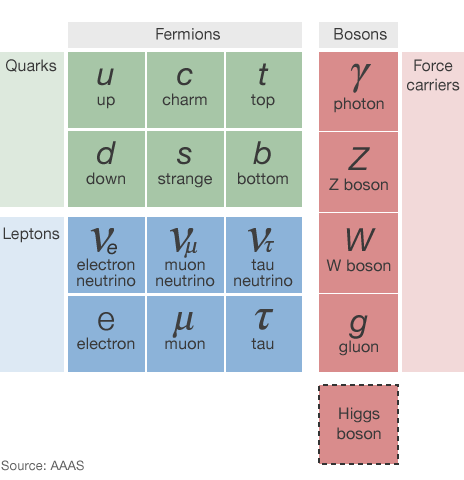
\includegraphics[width=0.6\linewidth]{Figures/higgs-elementary-particles.png}
\caption[The particles in the Standard Model]{The particles in the Standard Model. They are split into the bosons and fermions, with the fermions being further split into three generations of quarks and leptons.}
\label{fig:StandardModel}
\end{figure}

\subsection{Leptons}
Of greatest interest here for the work in this thesis are the particles known as leptons.
These leptons come in 6 flavors: the electron, muon, tau, electron neutrino, the muon neutrino, and the tau neutrino.
These particles interact with one another via the W and Z bosons and is discussed in more detail in \autoref{sec:Beta Decay}. 
When the Standard Model was first introduced in the 1960's, the neutrinos were assumed to be massless.
This was due to the fact that, as shown in \autoref{fig:NeutrinoMasses}, the masses of neutrinos are at least a million times lighter than the next-lightest particle, the electron with mass $0.511 \textrm{MeV}$
\footnote{Natural units, e.g. $c=1$ and $\hbar=1$, will be used throughout this thesis.
In this way, masses (units $\textrm{eV}/\textrm{c}^2$) and temperatures will be expressed in terms of energy, $\textrm{eV}$. 
Later on in the thesis, SI units will also be used, but the context of the units will make the convention clear.}.

\begin{figure}[tbph]
\centering
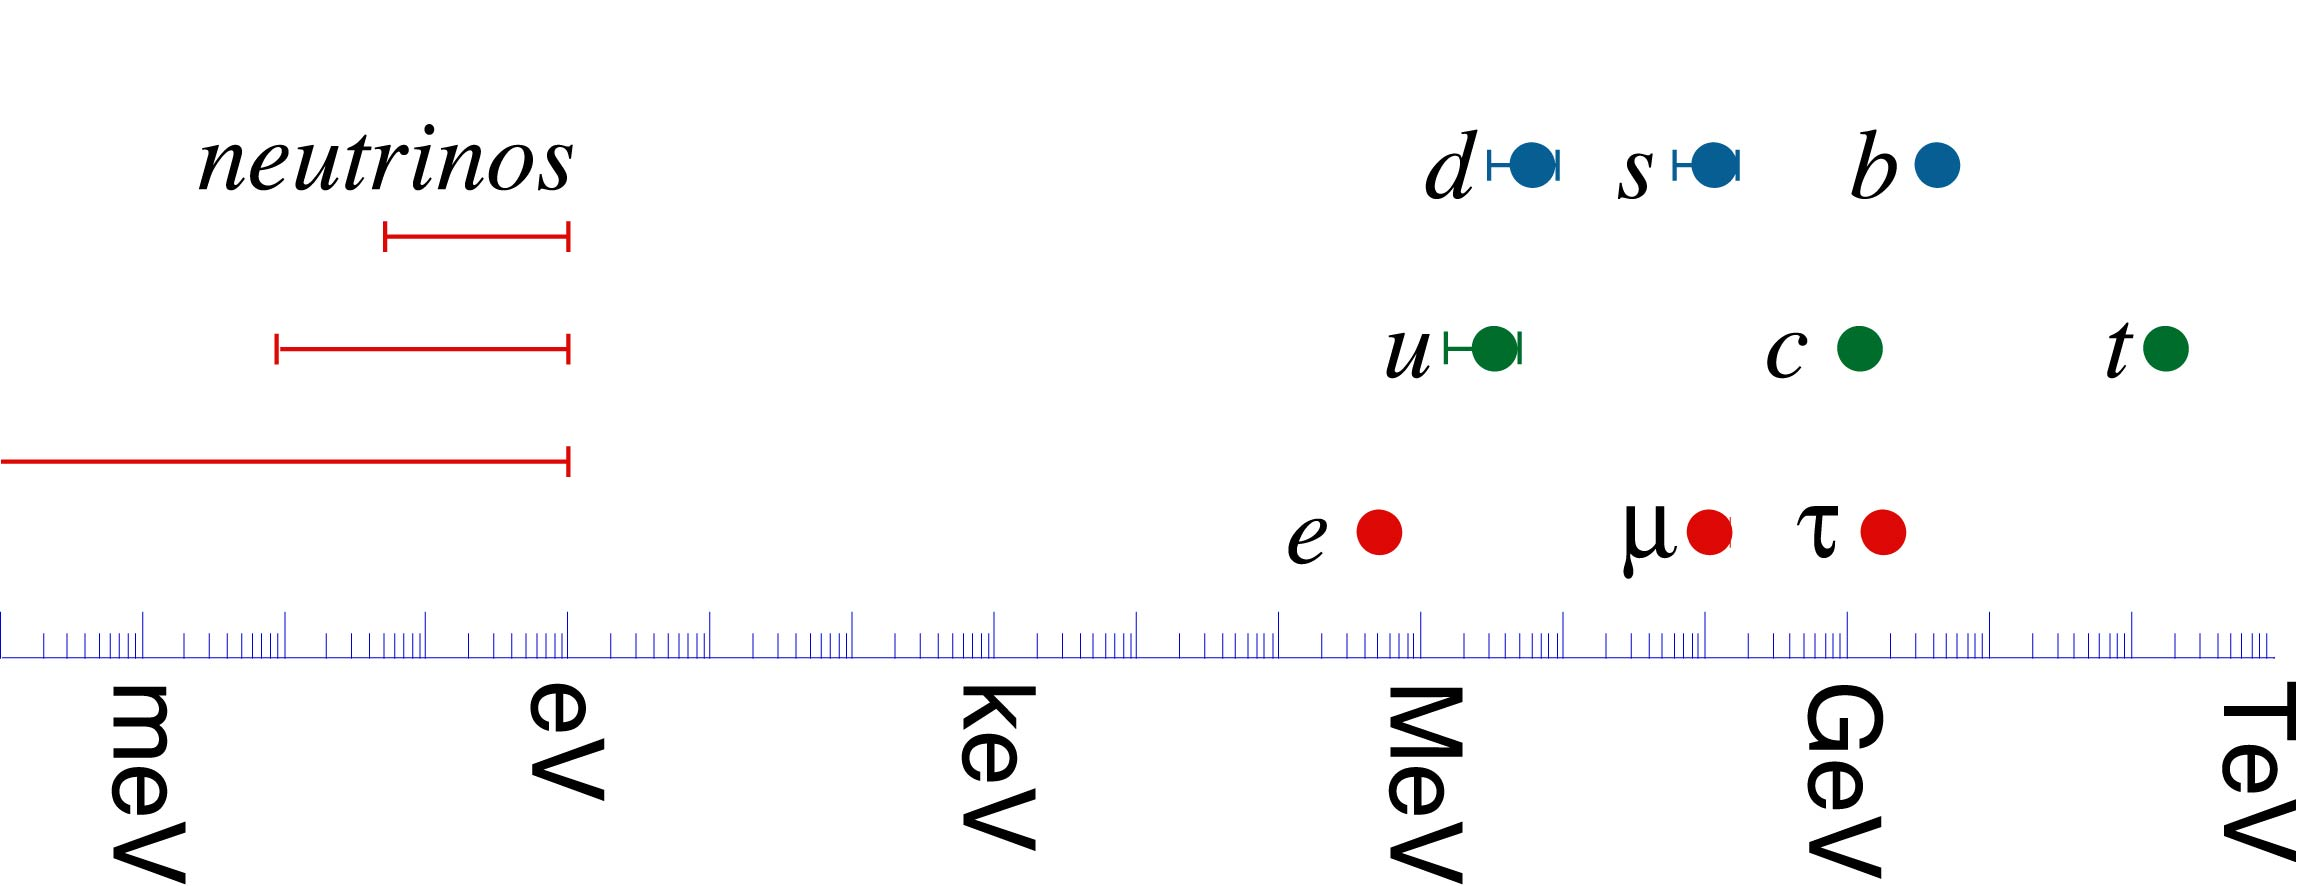
\includegraphics[width=0.9\linewidth]{Figures/NeutrinoMasses.jpg}
\caption[The masses of the fundamental fermion particles]
{The masses of the fundamental fermion particles.
The neutrinos are multiple orders of magnitude lighter than even their lightest counterparts.}
\label{fig:NeutrinoMasses}
\end{figure}

\subsubsection*{Neutrino Masses and Oscillation}
\label{ssec:NeutrinoMassesandOscillation}
The assumption that neutrinos were massless was shown to be incorrect, however, after they were observed to oscillate between their generational counterparts, namely $\nu_{\textrm{\alpha}} \leftrightarrow \nu_{\textrm{\beta}}$, where $\alpha$ and $\beta$ correspond to two different flavor states of the neutrino \cite{PhysRevLett.20.1205, Hatakeyama:1998ea, Ahmad:2001an}.
Not only does this phenomenon imply that the neutrinos have non-zero mass, it also shows that the neutrino flavor eigenstates are not equivalent to their mass eigenstates.
This transformation between the flavor and mass bases can be represented as a matrix, called the Pontecorvo–-Maki–-Nakagawa–-Sakata (PMNS) matrix 

\begin{equation}\label{eq:PMNS Matrix U Form}
\begin{bmatrix}
\nu_{e} \\
\nu_{\mu} \\
\nu_{\tau}
\end{bmatrix}
=
  \begin{bmatrix}
    U_{e1} & U_{e2} & U_{e3} \\
    U_{\mu1} & U_{\mu2} & U_{\mu3} \\
    U_{\tau1} & U_{\tau2} & U_{\tau3}
  \end{bmatrix}
  \begin{bmatrix}
  	\nu_{1} \\
	\nu_{2} \\
	\nu_{3}
  \end{bmatrix}
  \end{equation}
which unitarily transforms between the two bases.
In this formalism, the probability for measuring an electron neutrino to have the mass associated with the $\nu_1$ state is $|U_{e1}|^2$. The notation usually used to differentiate the $\nu_1$, $\nu_2$, and $\nu_3$ states is in decreasing order of the probability for a $\nu_i$ state to be observed in a $\nu_e$ state.
These probabilities are shown in \autoref{fig:Oscillations_electron_long}.
The PMNS matrix in \autoref{eq:PMNS Matrix U Form} can also be written as follows: 
\begin{equation}\label{eq:PMNS Matrix Standard Form}
  \begin{bmatrix}
    1 & 0 & 0 \\
    0 & c_{23} & s_{23} \\
    0 & -s_{23} & c_{23}
  \end{bmatrix}
  \begin{bmatrix}
  c_{13} & 0 & s_{13}e^{-i\delta_{CP}} \\
  0 & 1 & 0 \\
  -s_{13}e^{i\delta_{CP}} & 0 & c_{13}
  \end{bmatrix}
  \begin{bmatrix}
  c_{12} & s_{12} & 0 \\
  -s_{12} & c_{12} & 0 \\
  0 & 0 & 1
  \end{bmatrix}
  \begin{bmatrix}
  e^{i\alpha_1/2} & 0 & 0 \\
  0 & e^{i\alpha_2/2} & 0 \\
  0 & 0 & 1
  \end{bmatrix}
\end{equation}
where $s_{ij}$ and $c_{ij}$ are $\sin(\theta_{ij})$ and $\cos(\theta_{ij})$, respectively.
While this formulation in \autoref{eq:PMNS Matrix Standard Form} looks more complicated than the formulation in \autoref{eq:PMNS Matrix U Form}, it reduces the total number of parameters to just three mixing angles and a complex phase ($\theta_{12}$, $\theta_{13}$, $\theta_{23}$, and $\delta_{CP}$, respectively) due to the fact that five of these parameters can be absorbed into the phases of the lepton fields \cite{Valle:2006}.
The other parameters, $\alpha_1$ and $\alpha_2$, only play a role if the neutrino is a Majorana particle, which is discussed more in \autoref{ssec:Dirac and Majorana Masses}.
In any case, these values for $\alpha_1$ and $\alpha_2$ do not play a role in neutrino oscillation and their matrix can be thought of as the identity matrix in this scenario \cite{BILENKY1980495}.
To understand what this means for the behavior of neutrinos, a simpler model with only two neutrinos can be used.
In this simplified model with two neutrinos of flavor $\alpha$ and $\beta$, the usefulness of these angles and phases becomes apparent as \autoref{eq:PMNS Matrix Standard Form} appears as
\begin{equation}
\begin{bmatrix}
\nu_\alpha \\
\nu_\beta 
\end{bmatrix}
=
\begin{bmatrix}
\cos(\theta) & \sin(\theta) \\
-\sin(\theta) & \cos(\theta) 
\end{bmatrix}
\begin{bmatrix}
\nu_1 \\
\nu_2 
\end{bmatrix}.
\end{equation}
The probability that a neutrino has oscillated from type $\alpha$ to type $\beta$ after some time, $t$, is given as 
\begin{align}
P(\nu_\alpha\rightarrow\nu_\beta) &= \lvert<\nu_\beta(t)| \nu_\alpha>\rvert^2.
\end{align}
In the mass eigenstate, neutrinos propagate as plane waves of the form
\begin{align}
|v_i(t)>&=e^{i(Et-\vec{x}\cdot\vec{p})}|v_i(0)>.
\label{eq:OscillationProbability_general}
\end{align}
Neutrinos that are observed in the laboratory are generally produced in either a nuclear decay or a high-energy collision and have energies much larger than their rest mass.
For example, a neutrino produced in the sun can have energy up to 15 MeV.
Therefore, since $E >> m$, a relativistic approximation can be made in that $t\approx L$, where $L$ is the distance that the neutrino travels from the sun to the earth, and the energy of the neutrino can be expanded as follows:
\begin{align}
E &\approx E+\frac{m_i^2}{2E}.
\label{eq:E_approx}
\end{align}
Using \autoref{eq:E_approx} and \autoref{eq:OscillationProbability_general}, the probability of a neutrino oscillating from type $\alpha$ to a different type $\beta$ is then
\begin{align}
P(\nu_\alpha\rightarrow\nu_\beta) = 2 \sin^2(2\theta)\sin^2(\frac{\Delta m_{ij}^2L}{4E})
\label{eq:OscillationProbability_2nu}
\end{align}
where $\Delta m_{ij} = m_i^2 - m_j^2$, the mass-squared difference in the masses of the neutrino. For the three flavors of neutrinos: electron, $\mu$, and $\tau$ observed in nature, an example oscillation of an initially pure electron neutrino sample is shown in \autoref{fig:Oscillations_electron_long}.
\begin{figure}[tbph]
\centering
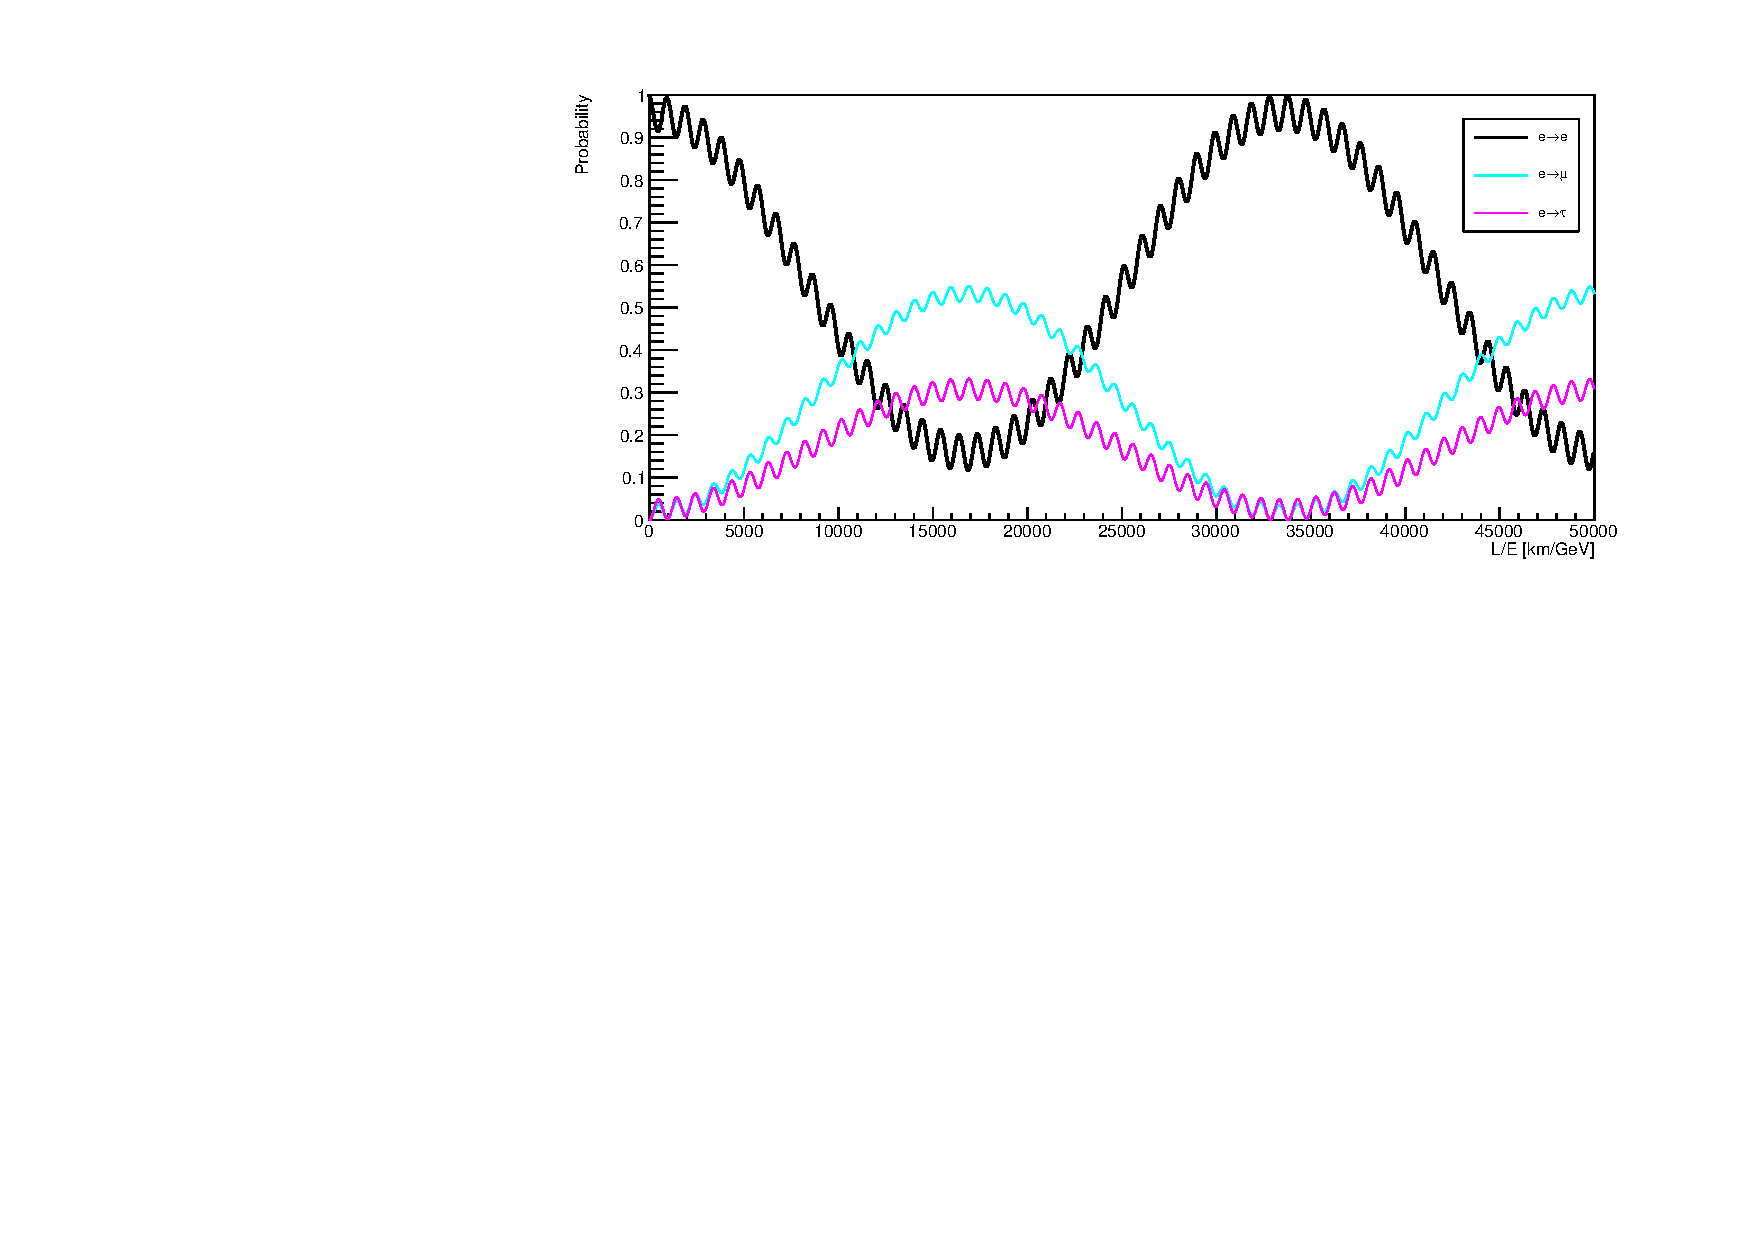
\includegraphics[width=0.95\linewidth]{Figures/Oscillation_2017Params_0CP.pdf}
\caption[Neutrino oscillation for an initial electron neutrino for 3 flavors of neutrino]
{Neutrino oscillation for an initial electron neutrino for 3 flavors of neutrino.
This plot is generated via the latest parameters in \cite{Patrignani:2016xqp} assuming normal hierarchy. 
For this plot, $\delta_{CP}$ has been set to zero for illustrative purposes, but a value of 0 (or 2$\pi$) is disfavored at the 2.4$\sigma$ level.}
\label{fig:Oscillations_electron_long}
\end{figure}

Even with the latest data from neutrino oscillation experiments, the exact masses of the neutrinos cannot be determined.
This can be seen in \autoref{eq:OscillationProbability_2nu} where only the relative masses of the neutrinos play a role, not their absolute masses. 
Other data, however, can set limits on the absolute mass scale of the neutrinos.
Using data derived from the Cosmic Microwave Background and baryon acoustic oscillations \cite{refId0}, the sum of the neutrino masses can be limited to, at 95\% C.L., $\sum_j m_j < 0.170~\textrm{eV}$, but there are existing models of neutrino mass generation where this result may not effectively constrain the neutrino mass \cite{Koksbang:2017rux} \cite{PhysRevLett.94.111801}.
Results from direct mass measurement experiments such as the Troitsk and Mainz experiments limit the electron antineutrino mass to, at 95\% C.L., $m_{\bar{\nu}_e} < 2.05~\textrm{eV}$ and $m_{\bar{\nu}_e} < 2.3~\textrm{eV}$, respectively \cite{Aseev:2011dq} \cite{Kraus:2004zw}, in a model-independent way.
Other upcoming experiments, KATRIN and Project 8, aim to measure these values with sensitivity up to 0.20 eV  and 0.04 eV, respectively \cite{Robertson:2013ziv} \cite{Esfahani:2017dmu}.

Another reason that \autoref{eq:OscillationProbability_2nu} is insensitive to the neutrino masses comes from the fact that the probabilities are unaffected by the sign of $\Delta m^2$.
However, this probability is for the propagation of a neutrino through vacuum, but in matter-dense regions, such as the sun, this probability is no longer correct.
This Mikheyev-Smirnov-Wolfenstein effect has been observed in solar neutrino measurements and allows for the determination that $\Delta m_{21}^2>0$ \cite{1367-2630-6-1-139, PhysRevD.17.2369}.
The sign of $\Delta m_{32}^2$ is still unknown, although long-baseline experiments of neutrino oscillation through the Earth aim to determine this effect.
Because of this, there are two possible scenarios for neutrino mass ordering, either $m_1 < m_2 < m_3$, called Normal Hierarchy (NH), or $m_3 < m_1 < m_2$, called Inverted Hierarchy (IH), shown in \autoref{fig:neutrinosfigs3nuspic}.
Recent results from the NOvA experiment point towards a NH Universe, but there is nothing yet to conclusively answer this question. \cite{Adamson:2017gxd}.
\begin{figure}[tbph]
\centering
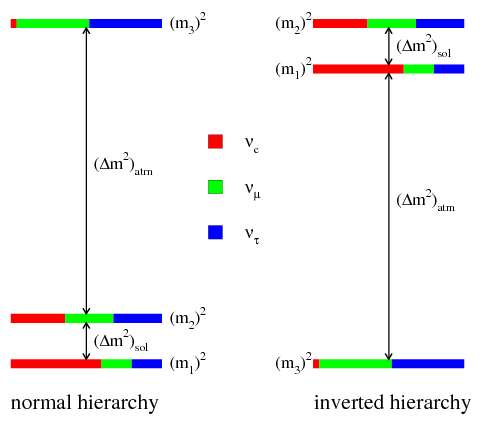
\includegraphics[width=0.8\linewidth]{Figures/Neutrinos_figs_3nuspic.png}
\caption[The mass orderings in both normal and inverted hierarchy]
{The mass orderings in both normal and inverted hierarchy.
The sign of $(\Delta m^2)_{\textrm{atm}}$ is not known, which causes the difference between the two scenarios.
Figure from \cite{Hewett:2012ns}.}
\label{fig:neutrinosfigs3nuspic}
\end{figure}

\subsection{Dirac and Majorana Masses}
\label{ssec:Dirac and Majorana Masses}

With the mass of neutrinos shown to be non-zero, the Standard Model can be extended to include the masses for the neutrinos, but this opens up another question for how exactly the neutrino mass comes in to the Standard Model Lagrangian.
For the other fundamental fermionic particles, e.g. the electron that has charge $\textrm{e}^-$, the corresponding antiparticle will have the opposite charge, e.g. the positron with charge $\textrm{e}^+$ charge.
This, therefore, means that the particle and antiparticle are distinct particles.
The neutrino is unique in this regard as it is the only electrically neutral fundamental fermion, meaning the neutrino may be identical to its own antiparticle.
Fermions that are not identical to their own antiparticles, e.g. electrons and up quarks, are called Dirac fermions, while fermions that are identical to their own antiparticles are called Majorana fermions.
These two types of fermions have their masses arise in different ways in the Standard Model.

A particle with a Dirac mass appears in the Standard Model Lagrangian as
\begin{align}
\mathcal{L} &= -m(\bar{\psi_L}\psi_R + \bar{\psi_R}\psi_L) \\
&= -m\bar{\psi_L}\psi_R + h.c.,
\label{eq:DiracMass_chiral}
\end{align}
after decomposing the spinor, $\psi$, into its left- and right-handed chiral states.
In order to make the above expressions clearer by taking the assumption that a particle's mass is derived purely from the Dirac term, the field is given by
\begin{equation}
\psi = \psi_L + \psi_R,
\end{equation}
\autoref{eq:DiracMass_chiral} can be rewritten as
\begin{align}
\mathcal{L} &= -m\bar{\psi}\psi. \label{eq:DiracMass}
\end{align}

For a Majorana particle, the mass term does not couple between left- and right-handed chiral states and appears solely as single-handed fields $\psi_L$ and the charge conjugate $\psi_L^c$ as follows,
\begin{align}
\mathcal{L}_L &= -\frac{1}{2}m_L\bar{\psi^c_L}\psi_L+h.c. \label{eq:MajoranaMass_chiral} \\
\mathcal{L}_R &= -\frac{1}{2}m_R\bar{\psi^c_R}\psi_R+h.c.
\end{align}
What can be seen from \autoref{eq:DiracMass} and \autoref{eq:MajoranaMass_chiral} is that when the term in \autoref{eq:DiracMass} acts on a particle $\psi$, it leaves the particle as a $\psi$, but when the term in \autoref{eq:MajoranaMass_chiral} acts on a particle $\psi$, it converts the particle into its antiparticle $\bar{\psi}$.
If we assign a `lepton number' of $+1$ for particles and $-1$ for antiparticles, then the Dirac mass term conserves lepton number while the Majorana mass term does not.

However, a particle need not be purely Dirac or Majorana. In general, a particle can have both mass terms due to other interactions such as the seesaw mechanism described in \autoref{sssec:Seesaw Mechanism}. In this case, the Lagrangian contains both the Dirac and Majorana terms as follows:
\begin{align}
\mathcal{L} = & -\frac{1}{2}m_D(\bar{\psi}_L\psi_R+\bar{\psi}^c_L\psi^c_R)+m_L\bar{\psi}_L\psi^c_R+m_R\bar{\psi}^c_L\psi_R +h.c. \\
\mathcal{L} = &\frac{1}{2} \begin{pmatrix}
\bar{\psi}_L,& \bar{\psi}^c_L \\
\end{pmatrix} \begin{pmatrix}
m_L & m_D \\
m_D & m_R
\end{pmatrix}
\begin{pmatrix}
\psi^c_R \\
\psi_R
\end{pmatrix}.
\label{eq:DiracAndMajoranaMass}
\end{align}

\subsubsection{Seesaw Mechanisms}
\label{sssec:Seesaw Mechanism}
While \autoref{eq:DiracAndMajoranaMass} is a Lagrangian that accounts for both Dirac and Majorana masses, it is not immediately obvious from where this mechanism arises.
For example, the masses of the other particles in the Standard Model arise from the Higgs mechanism.
However, if the masses of the neutrinos were a result of the same Higgs mechanism as the other fermions, the Yukawa coupling between neutrinos and the Higgs would have to be a surprisingly small number, $\lesssim 10^{-11}$, so there should be some other mechanism that can explain the mass scale of the neutrinos \cite{Merle:2013gea}.
In addition, while the Standard Model can be modified to include neutrino oscillations, this addition does not offer any explanation of why the mass of the neutrino is of order $10^6$ times lighter than the electron, the next lightest known fundamental particle.
However, the addition of a Majorana nature for neutrinos could be the cause of this difference and explain the million times lower mass.
One of the simplest methods in which the observed mass of the neutrinos could be realized is known as the seesaw mechanism \cite{PhysRevD.22.2227}.
This name is derived from the fact that, in this model, the left-handed light neutrinos are balanced out by the existence of more massive particles.
There are two main types of models for this mechanism, called the type-I and type-II seesaw mechanisms.
In the type-I seesaw mechanism, shown in \autoref{fig:TypeISeesawMechanism}, the neutrino mass is generated through fermion exchange, e.g. with the addition of heavy right-handed neutrinos, and in the type-II mechanism, shown in \autoref{fig:TypeIISeesawMechanism}, scalar boson exchange generates the neutrino mass.
The model most commonly considered in the field of \zeronubb~is the type-I seesaw mechanism and is discussed in greater detail in \autoref{sec:Neutrinoless Double Beta Decay}.
\begin{figure}[tbph]
\centering
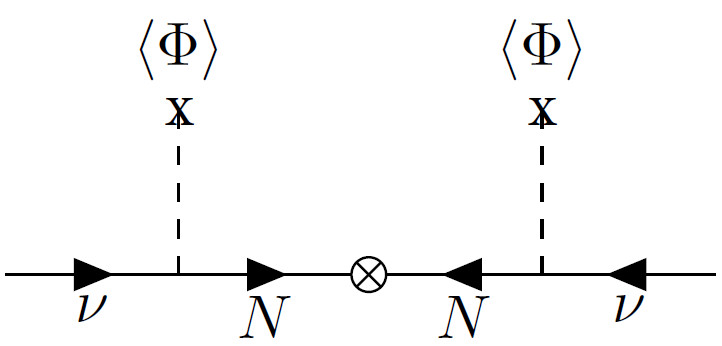
\includegraphics[width=0.40\linewidth]{Figures/TypeISeesaw.png}
\caption[Type-I seesaw mechanism]
{The type-I seesaw mechanism for neutrino mass generation wherein right-handed neutrinos, labelled $\textrm{N}$, contribute to the mass of the neutrinos.
Figure adapted from \cite{MIRANDA2016436}.}
\label{fig:TypeISeesawMechanism}
\end{figure}
The type-I seesaw mechanism with right-handed neutrinos then introduces a mass matrix for the neutrinos as follows:
\begin{equation}
M =\begin{pmatrix}
0 & m_D \\
m_D & M_R
\end{pmatrix}.
\end{equation}
If we take that the Dirac mass occurs for neutrinos in the same manner as for the other leptons in the Standard Model, i.e. due to electroweak symmetry breaking and the Higgs mechanism, then we can predict the value of the mass of the right-handed neutrinos.
In the case where $M_R \gg m_D$, the two neutrino masses become $M_R$ and $\frac{m_D^2}{M_R}$.
Taking $m_D$ to be $\approx1~\textrm{MeV}$, a meV-scale neutrino exists with a heavy right-handed neutrino of mass $10^{15}~\textrm{eV}$.

\begin{figure}[tbph]
    \centering
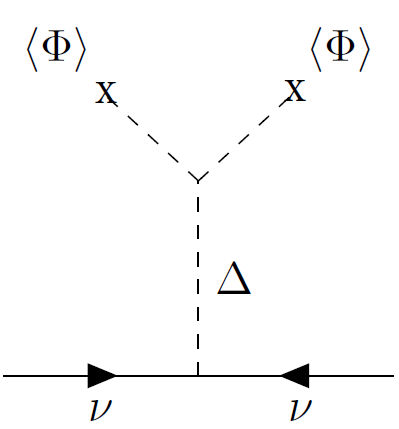
\includegraphics[width=0.40\linewidth]{Figures/TypeIISeesaw.png}
    \caption[Type-II seesaw mechanism]
    {The type-II seesaw mechanism for neutrino mass generation wherein a boson, labelled $\Delta$, contributes to the mass of the neutrinos.
    Figure adapted from \cite{MIRANDA2016436}.}
    \label{fig:TypeIISeesawMechanism}
\end{figure}


\section{Baryogenesis}
If the neutrino is demonstrated to have a Majorana mass, there are possible far-reaching implications to the evolution of the early universe.
In particular, after the Big Bang, matter and antimatter should have been produced in equal amounts; however, the matter in the universe dominates the antimatter, evidenced by measurements of the observable universe showing that is is purely matter on large scales.
For example, if there were antimatter galaxies or sectors of the universe, we would be able to observe large releases of energy due to matter-antimatter annihilation from collisions of galaxies or if there were an antimatter-dominated region of the universe due to annihilations at the border between the matter and antimatter regions.
This implies that the universe has a preference for slightly more baryons than antibaryons \cite{Canetti:2012zc}.
The requirements for a process to create this asymmetry are summed up in the Sakharov conditions for baryogenesis \cite{Sakharov:1967dj}:
\begin{enumerate}
\item Violation of baryon number, B
\item Violation of charge, C, and charge parity, CP
\item The asymmetry needs to be generated out of thermal equilibrium
\end{enumerate}
The first condition is needed so that there is a physics process within which a baryon can be created or an anti-baryon destroyed.
Assigning baryons such as protons and neutrons $\textrm{B}=1$, antibaryons $\textrm{B}=-1$, and non-baryonic matter $\textrm{B}=0$, this constraint can be written as $\Delta \textrm{B}\neq0$.
On its own, baryon number violation is not enough to create an imbalance between matter and antimatter as a process that has $\Delta\textrm{B}\neq0$ could just be reversed and prevent an asymmetry from forming.
Therefore, the second condition requires that a process with $\Delta\textrm{B}\neq0$ occurs more often for baryon creation or anti-baryon destruction than the reverse, i.e., $\Gamma(\Delta \textrm{B}>1) > \Gamma(\Delta \textrm{B}<-1)$.
Finally, the third condition requires that the process has to occur when the universe is not in thermal equilibrium as other processes would have to oppose whatever process satisfies the first two Sakharov conditions due to CPT (charge, parity, and time reversal) symmetry.

Therefore, in order to determine what caused the universe to evolve from equal parts matter and antimatter into the matter-dominated universe we see today, processes which satisfy all three Sakharov conditions are needed.
In the framework of the Standard Model, Baryon number is not a fundamental symmetry such as electric charge and is merely an ``accidental" symmetry of the Lagrangian without an associated mediator like the photon.
While baryon number cannot be violated classically in the Standard Model Lagrangian, quantum effects, namely sphaleron processes, may violate it \cite{PhysRevLett.37.8, KUZMIN198536}.
While these effects satisfy the other two Sakharov conditions, there is enough of an effect to explain the measured asymmetry,
\begin{align}
\Delta &= \frac{N_B - N_{\bar{B}}} {N_B + N_{\bar{B}}} \biggr\rvert_{T \gtrsim 1~\textrm{GeV}}
\label{eq:BAU_earlyuniverse}
\end{align}
where $N_B$ and $N_{\bar{B}}$ are, respectively, the number of baryons and anti-baryons, when the asymmetry formed with the universe at a temperature of approximately 1 GeV.
This baryon asymmetry in the Universe can be inferred from the current abundance of baryons and photons in the universe at the current temperature of 0.2 meV.
In this way, \autoref{eq:BAU_earlyuniverse} can be written as
\begin{align}
    \Delta &\sim \eta = \frac{N_B}{N_\gamma} \biggr\rvert_{T = 0.2 meV}
    \label{eq:eta_lateuniverse}
\end{align}
as the main product of baryon-antibaryon annihilation are photons, given by $N_\gamma$, and the number of anti-baryons remaining in the universe is vanishingly small.
Calculations from fitting parameters due to Big Bang Nucleosynthesis from the abundance of light elements in the intergalactic medium and calculations from the Cosmic Microwave Background data both give values of $\eta\sim 10^{-10}$ \cite{Canetti:2012zc}.
However, the contributions to $\eta$ from Standard Model processes predict an $\eta$ of $10^{-20}$, far below the observed value.

\subsection{Majorana Neutrinos and Leptogenesis}
However, these sphaleron processes conserve another symmetry, namely. $\textrm{B}-\textrm{L}$, where L is the lepton number and has similar rules to the baryon number described above.
Therefore, a place to look for baryon number violation may be in the lepton sector.
In this case, the imbalance between matter and antimatter is due to an imbalance in leptons that transfers over to the baryons.
This `leptogenesis' would have to fulfill an analogous set of Sakharov conditions to that described above.
This violation is possible if the neutrino is its own antiparticle, for example, in the interaction $d + d \rightarrow u + u + e + e$ in \autoref{fig:0nuBB}, lepton number is violated by $\Delta\textrm{L}=2$.
\begin{figure}[tbph]
\centering
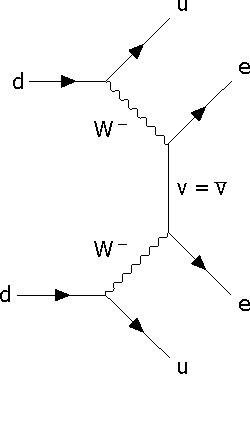
\includegraphics[width=0.35\linewidth]{Figures/0NuBB_clip.pdf}
\caption[The Feynman diagram for a lepton-number violating process]
{The Feynman diagram for a lepton-number violating process.
Two down quarks each convert to an up quark and emit a $\textrm{W}^{-}$ boson.
The two $\textrm{W}^{-}$ bosons then exchange a neutrino and emit an electron.
Note that this process is possible only if the neutrino is its own antiparticle.}
\label{fig:0nuBB}
\end{figure}
This method of lepton number violation would then also be associated with a baryon number violating process with $\Delta\textrm{B}=2$ as well.
To make this scenario of leptogenesis even more attractive as a candidate for baryon number asymmetry, the quantum effects that violate baryon number are unsuppressed at the high temperatures of the early universe.
Therefore, this lepton number violation could transfer to the baryon sector and result in the matter-dominated observable universe seen today.
\chapter{Double Beta Decay}
\label{chap:Beta Decay}

While a lepton-violating process such as that in \autoref{fig:0nuBB} would an incredible result to discover in the laboratory, it's not quite so simple as to obtain a ``soup" of down quarks and wait for them to decay into up quarks and electrons or to look at the time-reversed process and use electron beams to produce up and down quarks!
The way that an interaction such as the one shown above in \autoref{fig:0nuBB} could feasibly be discovered in a laboratory setting is through decays of nuclei, namely through neutrinoless double-beta decay, \zeronubb. 
\section{Beta Decay}
\label{sec:Beta Decay}
\zeronubb~decay is an extension on a well-known and well-understood process called beta decay. In beta decay, a decay that occurs in many nuclei, the number of protons, Z, in the nucleus changes while the number of total nucleons, A, is constant.
Beta decay occurs in two main processes and can be described in the following nuclear decays
\begin{align}
    (Z, A) & \rightarrow (Z+1, A)+\textrm{e}+\Bar{\nu}_e \label{eq:neutrondecay} \\
    (Z, A) & \rightarrow (Z-1, A)+\Bar{\textrm{e}}+\nu_e. \label{eq:protondecay}
\end{align}
\begin{figure}[tbph]
    \centering
    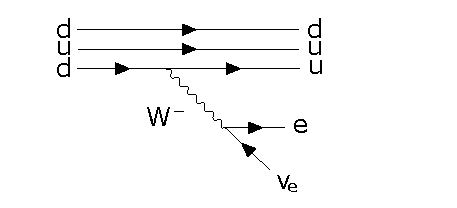
\includegraphics[width=0.8\linewidth]{Figures/NeutronBetaDecay.pdf}
    \caption[Beta Decay Feynman diagram for a neutron converting to a proton.]
    {The Feynman diagram for beta decay for a neutron to convert to a proton inside a nucleus by emitting an electron and and anti-neutrino.}
    \label{fig:NeutronBetaDecay}
\end{figure}
The process in \autoref{eq:neutrondecay} is shown in \autoref{fig:NeutronBetaDecay}, and the accompanying process, \autoref{eq:protondecay}, while kinematically forbidden in free protons because protons have less mass than neutrons, is able to occur in nuclei where the change in binding energies of the resultant nucleus is able to compensate for the mass difference between protons and neutrons.
When discussing these decays, an important value of interest is known as the Q-value of the decay which is the available energy released during the decay of one nucleus to another, namely (Z,A) $\rightarrow$ (Z$\pm1$, A).
This energy sets the maximum energy that can be carried off by the resultant particles and serves as the endpoint of the beta decay spectrum. 
\subsection{History of Beta Decay}
Historically, the discovery and physics advancements from double-beta decay has shed some light on new physics.
In particular, when the energy spectrum of beta decays was first discovered, it took the physics community by surprise that the spectrum was continuous and not peaked at a single value as, e.g., an alpha decay would be \cite{o.vonbayero.hahnl.meitner}.
This seemed to suggest one of two things. Either energy was not conserved in the interaction, or there was a seemingly massless undetected particle that was escaping the interaction and taking away energy.
To resolve this issue, Wolfgang Pauli speculated in a famous letter in 1930 to ``dear radioactive ladies and gentlemen" about the existence of the neutrino particle to account for the missing energy \cite{pauli_1930}.
At the time, the physics community was quite skeptical of such a theory, as it posited a particle that was seemingly impossible to detect in order to conserve energy, and Enrico Fermi was even rejected on these grounds from publishing his theory on beta decay in the journal Nature, publishing instead in a lesser-known journal \cite{fermi_1934}.
Despite the misgivings of the community, neutrinos were in fact not impossible to detect and were first discovered in the Cowan-Reines experiment only 20 years later in 1954 \cite{PhysRev.92.830}.
Using beta capture, a similar process to beta decay, this experiment observed antineutrinos interacting with ``free" protons in hydrogen atoms in a water tank. 
In this way, beta decay has been used to observe new physics and has been both an active and fruitful area of research since it was first observed.
Even recently, observations of neutrinos have resulted in the discovery of neutrino oscillations, discussed in \autoref{ssec:NeutrinoMassesandOscillation}, which was the first confirmation of physics beyond the Standard Model.
\section{Double-Beta Decay}
\label{sec:Double Beta Decay}
Since beta decay is an allowed process, a decay in which two decays happen simultaneously, double-beta decay, described in \autoref{eq:doubleneutrondecay} and \autoref{eq:doubleprotondecay} below, should also be allowed.
\begin{align}
    (Z, A) & \rightarrow (Z+2, A)+2\textrm{e}+2\Bar{\nu}_e \label{eq:doubleneutrondecay} \\
    (Z, A) & \rightarrow (Z-2, A)+2\Bar{\textrm{e}}+2\nu_e \label{eq:doubleprotondecay} 
\end{align}
However, for most nuclei, this second-order weak process is dwarfed by the significantly higher rates of single-beta decay.
Although the rate of beta decay depends greatly on the isotope, even some of the longest half-lives, such as that of $^{40}$K with a half-life of $1.251\times10^{9}~\textrm{yr}$, are many orders of magnitude faster than typical half-lives for double-beta decay, $\mathcal{O}(10^{20})~\textrm{yr}$.
This 11 orders of magnitude longer rate makes measuring double-beta decay virtually impossible as the single-beta decay rate presents an insurmountable background.
However, the exception to this occurs in some even-even nuclei wherein single beta decay is energetically forbidden, but double beta decay is allowed, shown in \autoref{fig:parabola_even}.
Of the 35 naturally-occurring isotopes where double beta decay is possible, 12 of them have been measured in the laboratory, and 9 of these are shown in \autoref{tab:2nuHalfLife}.
As the longest measured half-life of alpha decay is from $^{209}\textrm{Bi}$ with a half-life of $1.9 \times 10^{19}~\textrm{years}$ \cite{Marcillac:2003Bi-209detection}, double-beta decay half lives are the rarest nuclear decays that have been measured.
\begin{figure}[htbp]
%\captionsetup[subfigure]{justification=centering}
\centering
\begin{subfigure}[t]{0.40\textwidth}
\centering
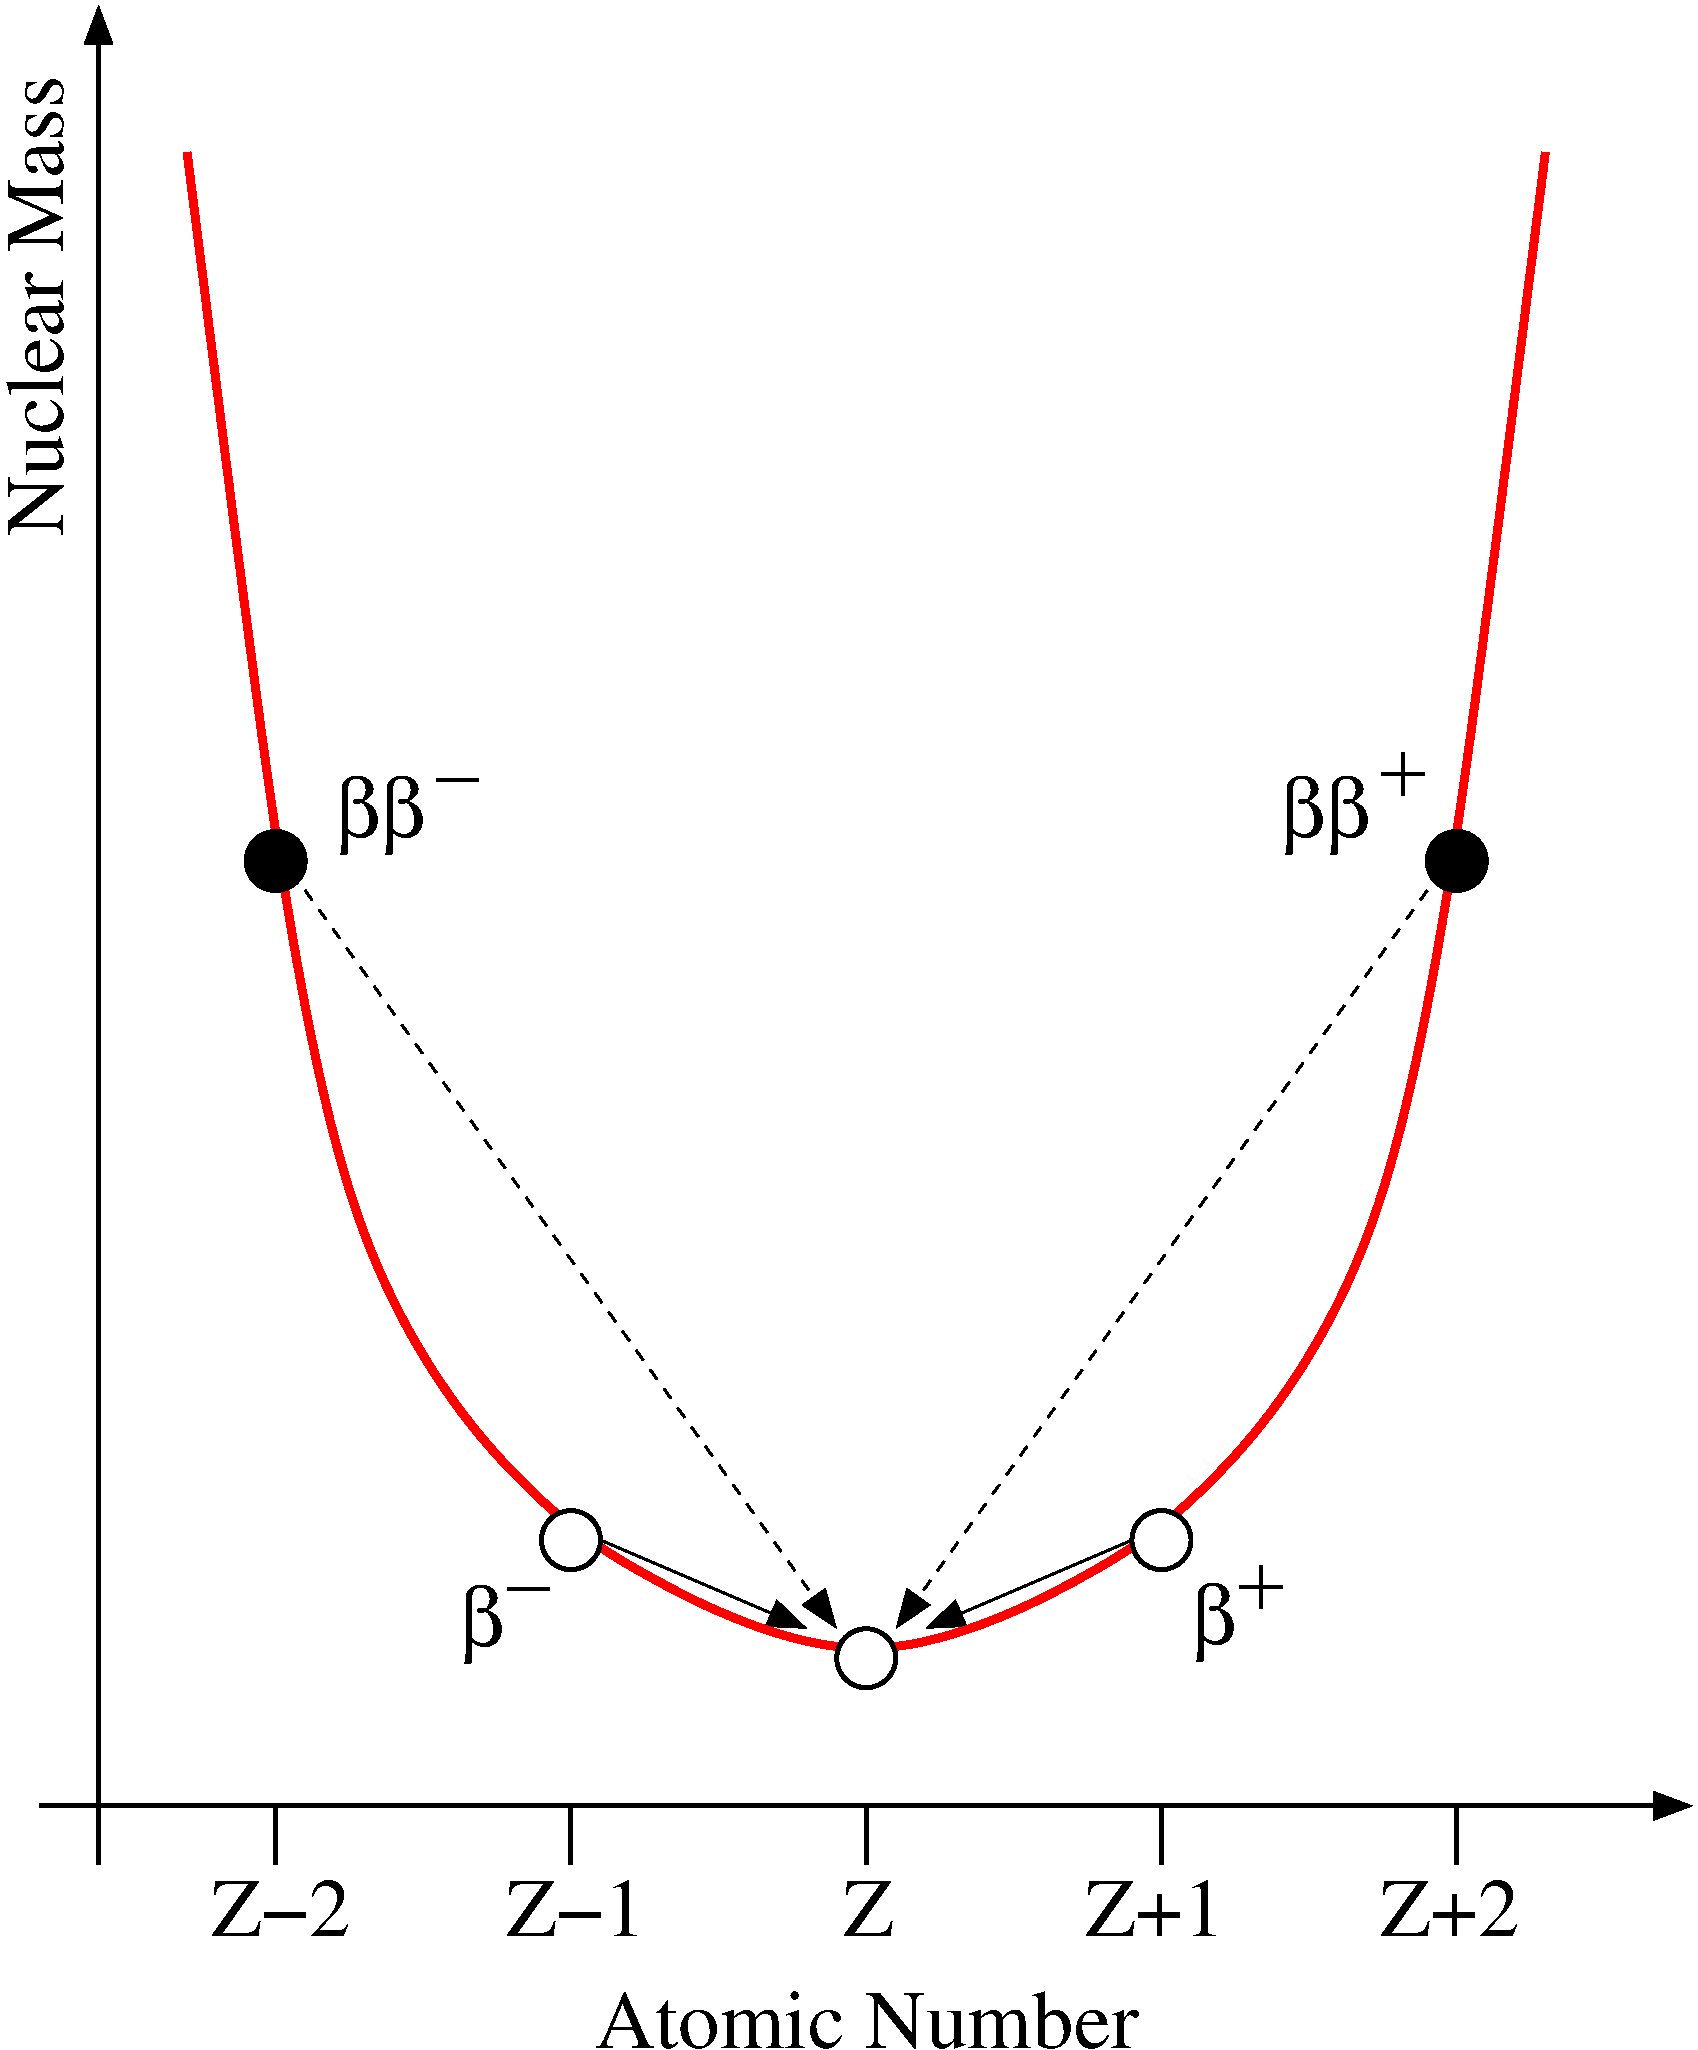
\includegraphics[width=0.9\textwidth]{Figures/parabola_odd_edited.pdf}
\caption{}
\label{fig:parabola_odd}
\end{subfigure}
\qquad
\begin{subfigure}[t]{0.40\textwidth}
\centering
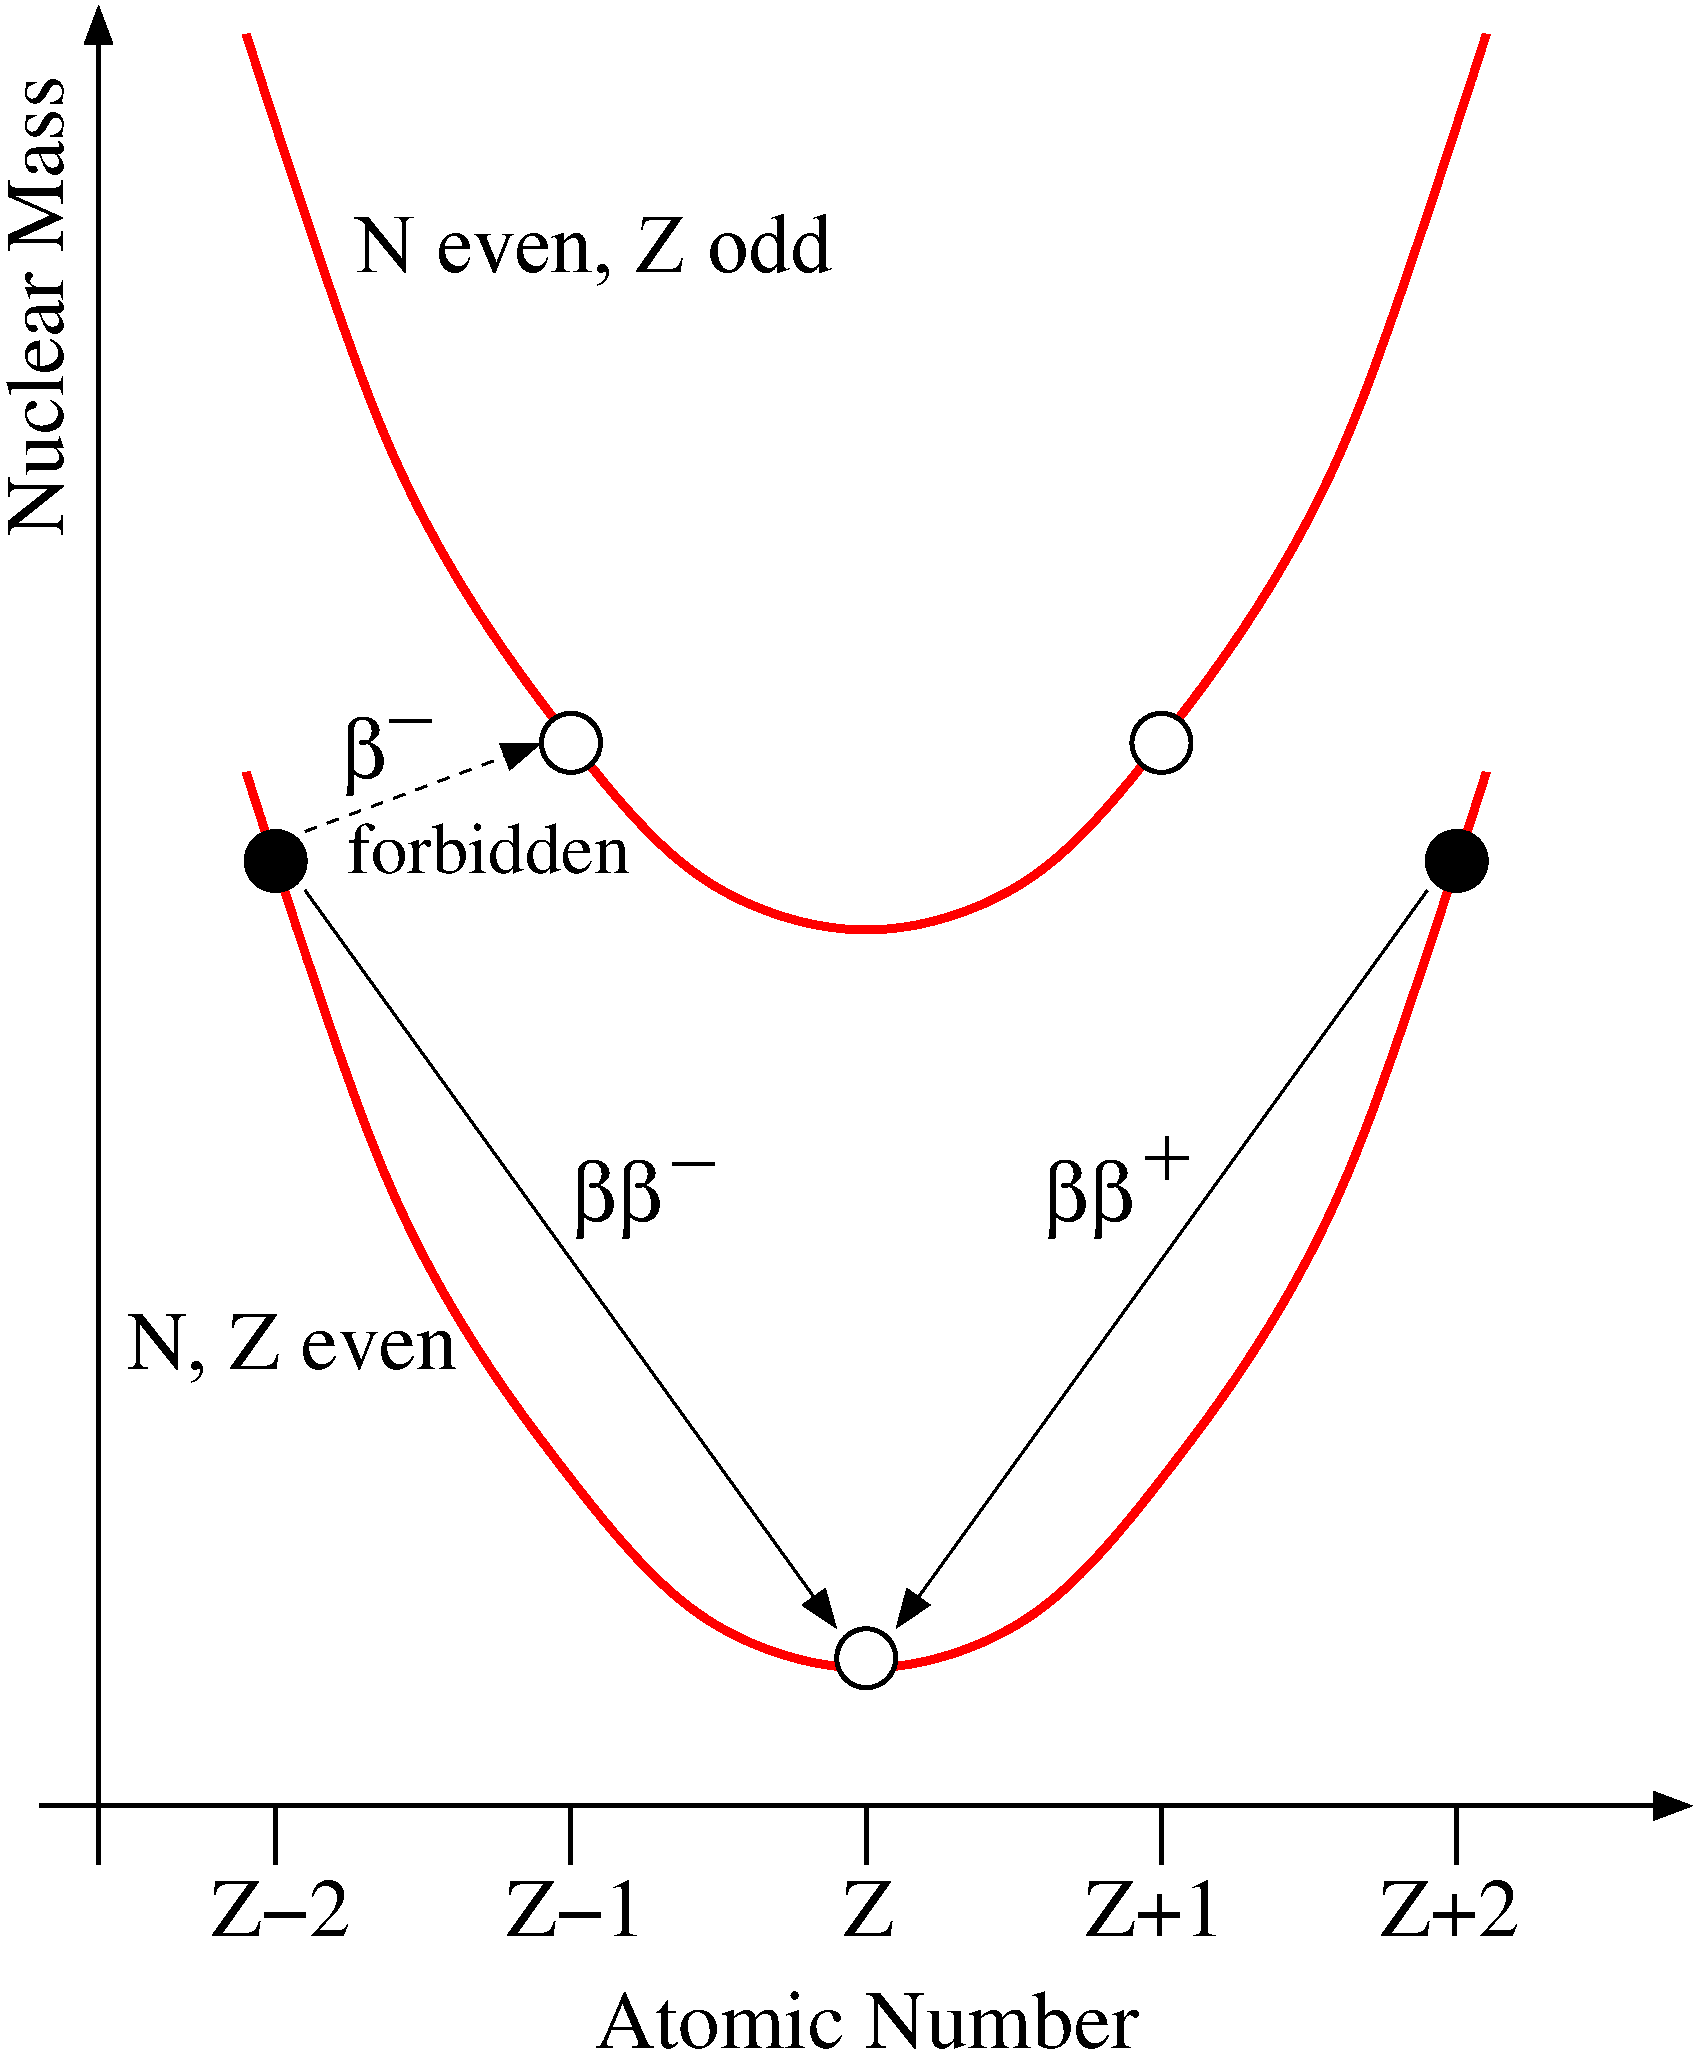
\includegraphics[width=0.9\textwidth]{Figures/parabola_even_edited.pdf}
\caption{}
\label{fig:parabola_even}
\end{subfigure}
\caption[Two sets of double-beta decay candidate nuclei.
(a) an odd mass nucleus allows for both single- and double-beta decay.
(b) an even-even nucleus allows only double-beta decay as single-beta decay is kinematically forbidden.]
{Two sets of double-beta decay candidate nuclei.
(a) an odd mass nucleus allows for both single- and double-beta decay.
(b) an even-even nucleus allows only double-beta decay as single-beta decay is kinematically forbidden.}
\label{fig:parabola_evenodd}
\end{figure}
\begin{table}[H]
\centering
\begin{tabular}{ccc}
\hline \hline
Isotope & Half-life, $10^{21}$ years & Experiment \\ \hline 
$^{48}\textrm{Ca}$ & $0.044^{+0.005}_{-0.004} \pm 0.004$\cite{Bongrand:2011ei} & Nemo-3 \\
$^{76}\textrm{Ge}$ & $1.926^{+0.025}_{-0.022} \pm 0.092$\cite{Agostini:2015nwa} & GERDA  \\
$^{82}\textrm{Se}$ & $0.096 \pm 0.003 \pm 0.010$\cite{Bongrand:2011ei} & NEMO-3 \\ 
$^{96}\textrm{Zr}$ & $0.0235 \pm 0.0014 \pm 0.0016$\cite{Bongrand:2011ei} & NEMO-3 \\ 
$^{100}\textrm{Mo}$ & $0.00711 \pm 0.00002 \pm 0.00054$\cite{Bongrand:2011ei} & NEMO-3 \\ 
$^{116}\textrm{Cd}$ & $0.028 \pm 0.001 \pm 0.003$\cite{Bongrand:2011ei} & NEMO-3 \\ 
%^{128}\textrm{Te}$ & $7200 \pm 400$ & Geochemical \\
$^{130}\textrm{Te}$ & $0.82 \pm 0.02\pm 0.06$\cite{Alduino:2016vtd} & CUORE-0 \\
$^{136}\textrm{Xe}$ & $2.165 \pm 0.016 \pm 0.059$\cite{Albert:2013gpz} & EXO-200 \\
$^{150}\textrm{Nd}$ & $0.00911^{+0.00025}_{-0.00022}\pm 0.00063$\cite{Bongrand:2011ei} & NEMO-3 \\
%$^{238}\textrm{U}$ & $2.0 \pm 0.6$ & Radiochemical \\
\hline \hline
\end{tabular} 
\caption[List of known two-neutrino beta decay half lives.]
{List of the known double-beta decay half lives along with the experiment which has the most precise measurement to date.
The order of the errors on the half-life are statistical followed by systematic.}
\label{tab:2nuHalfLife}
\end{table}
\section{Neutrinoless Double-Beta Decay}
\label{sec:Neutrinoless Double Beta Decay}
Of most interest to this thesis is a variation on the \twonubb~decay mentioned above where the neutrinos are exchanged during the decay and do not emerge as final state particles.
This corresponds to the decay shown in \autoref{fig:0nuBB} and in \autoref{eq:doubleneutrondecay_neutrinoless} and \autoref{eq:doubleprotondecay_neutrinoless} below:
\begin{align}
    (Z, A) & \rightarrow (Z+2, A)+2\textrm{e} \label{eq:doubleneutrondecay_neutrinoless} \\
    (Z, A) & \rightarrow (Z-2, A)+2\Bar{\textrm{e}}. \label{eq:doubleprotondecay_neutrinoless} 
\end{align}
In this decay, only possible if the neutrino has a Majorana mass, all of the available energy released in the decay is carried away by the electrons.
Therefore, a detector which can measure the electron energy would always reconstruct the decay energy to be precisely at the Q-value of the decay, in contrast to the energy spectrum from \twonubb~decay which is a continuum up to the Q-value due to the undetected neutrinos carrying energy away from the detectors.
\begin{figure}
    \centering
    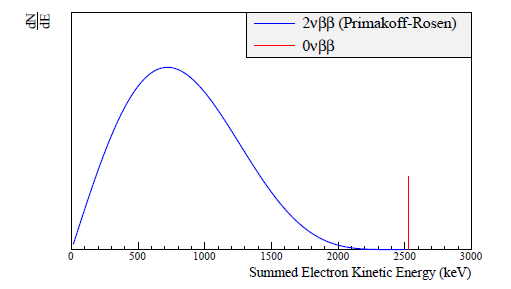
\includegraphics[width=0.6\linewidth]{Figures/2nuBBSpectrum.png}
    \caption[The energy spectrum for \twonubb~decay of $^{130}$Te along with the spectrum for \zeronubb.]
    {The energy spectrum for \twonubb~decay of $^{130}$Te along with the spectrum for \zeronubb.
    The spectrum for \zeronubb~is not shown to scale.
    Note that while the \twonubb~spectrum covers the entire range from 0 to the Q-value, in the case of \zeronubb, the energies are monoenergetic at the Q-value.}
    \label{fig:2nuSpectrum}
\end{figure}
The rate of \zeronubb~decay in particular nuclei can be expressed according to 
\begin{align}
    [T^{0\nu}_{1/2}]^{-1}&=\ln(2)G_{0\nu}|M_{0\nu}|^2|f(m_i,U_{ei})|^2
    \label{eq:halflife}
\end{align}
where the phase space factor, $G_{0\nu}$, is determined by the kinematics, $|M_{0\nu}|$ is the nuclear matrix element determined by the physics of each nucleus, and $|f(m_i, U_{ei})|$ is the determined by the underlying physics of the interaction and includes the masses $m_i$ and mixing matrix elements $U_{ei}$ of the neutrino species \cite{Barea:2013bz}.
As experiments searching for \zeronubb~are only truly sensitive to the half-life, any further statements on any other physical parameters contained in $|f(m_i, U_{ei})|$ require difficult calculations of $G_{0\nu}$ and $|M_{0\nu}|$.
In particular, there are many different theoretical models which calculate $|M_{0\nu}|$ for various isotopes, shown in \autoref{fig:NME}.
\begin{figure}[htbp]
    \centering
    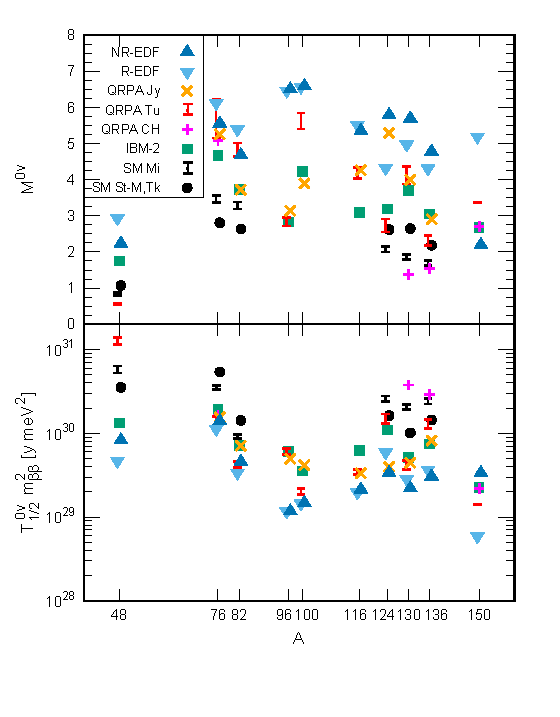
\includegraphics[width=0.8\linewidth]{Figures/NMEversusA.pdf}
    \caption[The various theoretically-determined nuclear matrix elements for selected \zeronubb~candidate isotopes.]
    {Top: The various theoretically-determined nuclear matrix elements for selected \zeronubb~candidate isotopes are shown.
    Bottom: The various models are in strong tension with one another and result in a large theoretical uncertainty for the half-life. Figure from \cite{Engel:NME}.}
    \label{fig:NME}
\end{figure}
Taking a model of light neutrino exchange, shown in \autoref{fig:0nuBB}, then $|f(m_i, U_{ei})|$ can be rewritten as
\begin{align}
        f(m_i, U_{ei})_{\textrm{light}} &= \frac{\langle m_{\beta\beta}\rangle}{m_e}
\end{align}
where $m_{\beta\beta}$ is the effective neutrino mass with
\begin{align}
    m_{\beta\beta}&=|\sum_iU^2_{ei}m_{\nu i}|.
    \label{eq:mbetabeta}
\end{align}
As the physical parameter $m_{\beta\beta}$ is isotope-independent, this becomes the figure-of-merit for comparing the results from experiments measuring the half-life of \zeronubb~decay from different isotopes. However, a large uncertainty is introduced due to the uncertainty in the nuclear matrix elements for each isotope.
In addition, possible values of $m_{\beta\beta}$ depend on the type of universe we are in, as shown in \autoref{fig:cuore-mbetabeta}.
If the masses of the neutrino obey inverted hierarchy, then the allowed values of $m_{\beta\beta}$ are within reach of current experiments with next-generation experiments being able to confidently rule out \zeronubb. However, for normal hierarchy, allowed values of $m_{\beta\beta}$ may be much lower. 
Due to the mono-energetic nature of \zeronubb, the sensitivity of an experiment can be determined from a few experimental parameters.
Each experiment can be reduced to a counting experiment in a window given by the energy resolution, $\Delta E$ of the experiment at the Q-value of \zeronubb.
For an experiment such as CUORE, with the source of \zeronubb~also acting as the detectors, the number of signal events, $S$, in some time, $t$, would be given by
\begin{align}
    S &= \ln(2)\frac{\epsilon\cdot N \cdot t}{T^{0\nu}_{1/2}}
    \label{eq:signal_betabeta}
\end{align}
where $\epsilon$ is the signal detection efficiency and $N$ is the number of nuclei able to undergo \zeronubb.
Similarly, for the number of background events, $B$, in the same interval is given by
\begin{align}
    B &= b\cdot M \cdot t \cdot \Delta E
    \label{eq:background_betabeta}
\end{align}
where $b$ is the background rate per unit energy per unit detector mass and $M$ is the total active mass of the detector.
If $\Delta E$ is sufficiently small that the irreducible background from \twonubb~decays does not appreciably factor into the background and the background is therefore externally sourced and obeys Gaussian statistics, a $1\sigma$ half-life sensitivity is then given by
\begin{align}
    T^{0\nu}_{1/2}=\ln(2)\frac{\epsilon \cdot a_I \cdot N_A \cdot \eta}{W} \sqrt{\frac{M\cdot t}{b\cdot \Delta E}},
    \label{eq:sensitivity_long}
\end{align}
with $\eta$ as the number of nuclei of interest per molecule of the detector, e.g. 1 for CUORE's \teotwo~crystals, and where the number of candidate nuclei from \autoref{eq:signal_betabeta} is rewritten as
\begin{align}
    N &=M\frac{a_I \cdot N_A\cdot \eta}{W}
\end{align}
taking into account isotopic abundance, $a_I$, of the decaying isotope and its molar mass, $W$ along with Avogadro's number, $N_A$.
For an experiment that searches for \zeronubb, maximizing this sensitivity is of paramount importance, and the most experimentally-relevant factors result in a common rewriting of the sensitivity as
\begin{align}
S &\propto a_I \sqrt{\frac{M \cdot t}{b \cdot \Delta E}}.
\label{eq:sensitivity_short}
\end{align}
This means that an experiment searching for \zeronubb~gains by increasing the isotopic abundance of the decay of interest, increasing its live-time, $M\cdot t$, decreasing its background, and improving its energy resolution.
Many experiments enrich their isotope of choice in order to increase their sensitivity, while CUORE benefits from the relatively high natural abundance of \teonethirty, shown in \autoref{fig:q_vs_ia-color}, and does not need to undergo the expense process of isotope enrichment.
A high Q-value also helps to decrease the background as \gamma~backgrounds generally decrease at higher energies and it is equally important to avoid other \gamma~peaks from decays near the Q-value.
For example, in CUORE, two \gamma~particles emitted from $^{60}\textrm{Co}$ decays may be absorbed simultaneously in a detector with an energy of approximately 2605 keV.
Since this is close the to the Q-value of 2528 keV for \teonethirty, this requires $\Delta E$ small enough to distinguish these background events from the possible signal.
CUORE's design goal of 5 keV resolution is more than enough to accomplish this.
In practice, experiments such as CUORE with a precise energy resolution suffer from having a segmented detector, as the materials used to hold the detectors in place also contribute to the background.
Other experiments such as those that search for \zeronubb~decay in $^{136}$Xe are able to scale up their mass much easier as it is all one continuous volume, but suffer from having significantly less precise energy resolution.
A further discussion of other experiments in the field is in \autoref{sec:State of Neutrinoless Double Beta Decay Experiments}.
\begin{figure}[htbp]
    \centering
    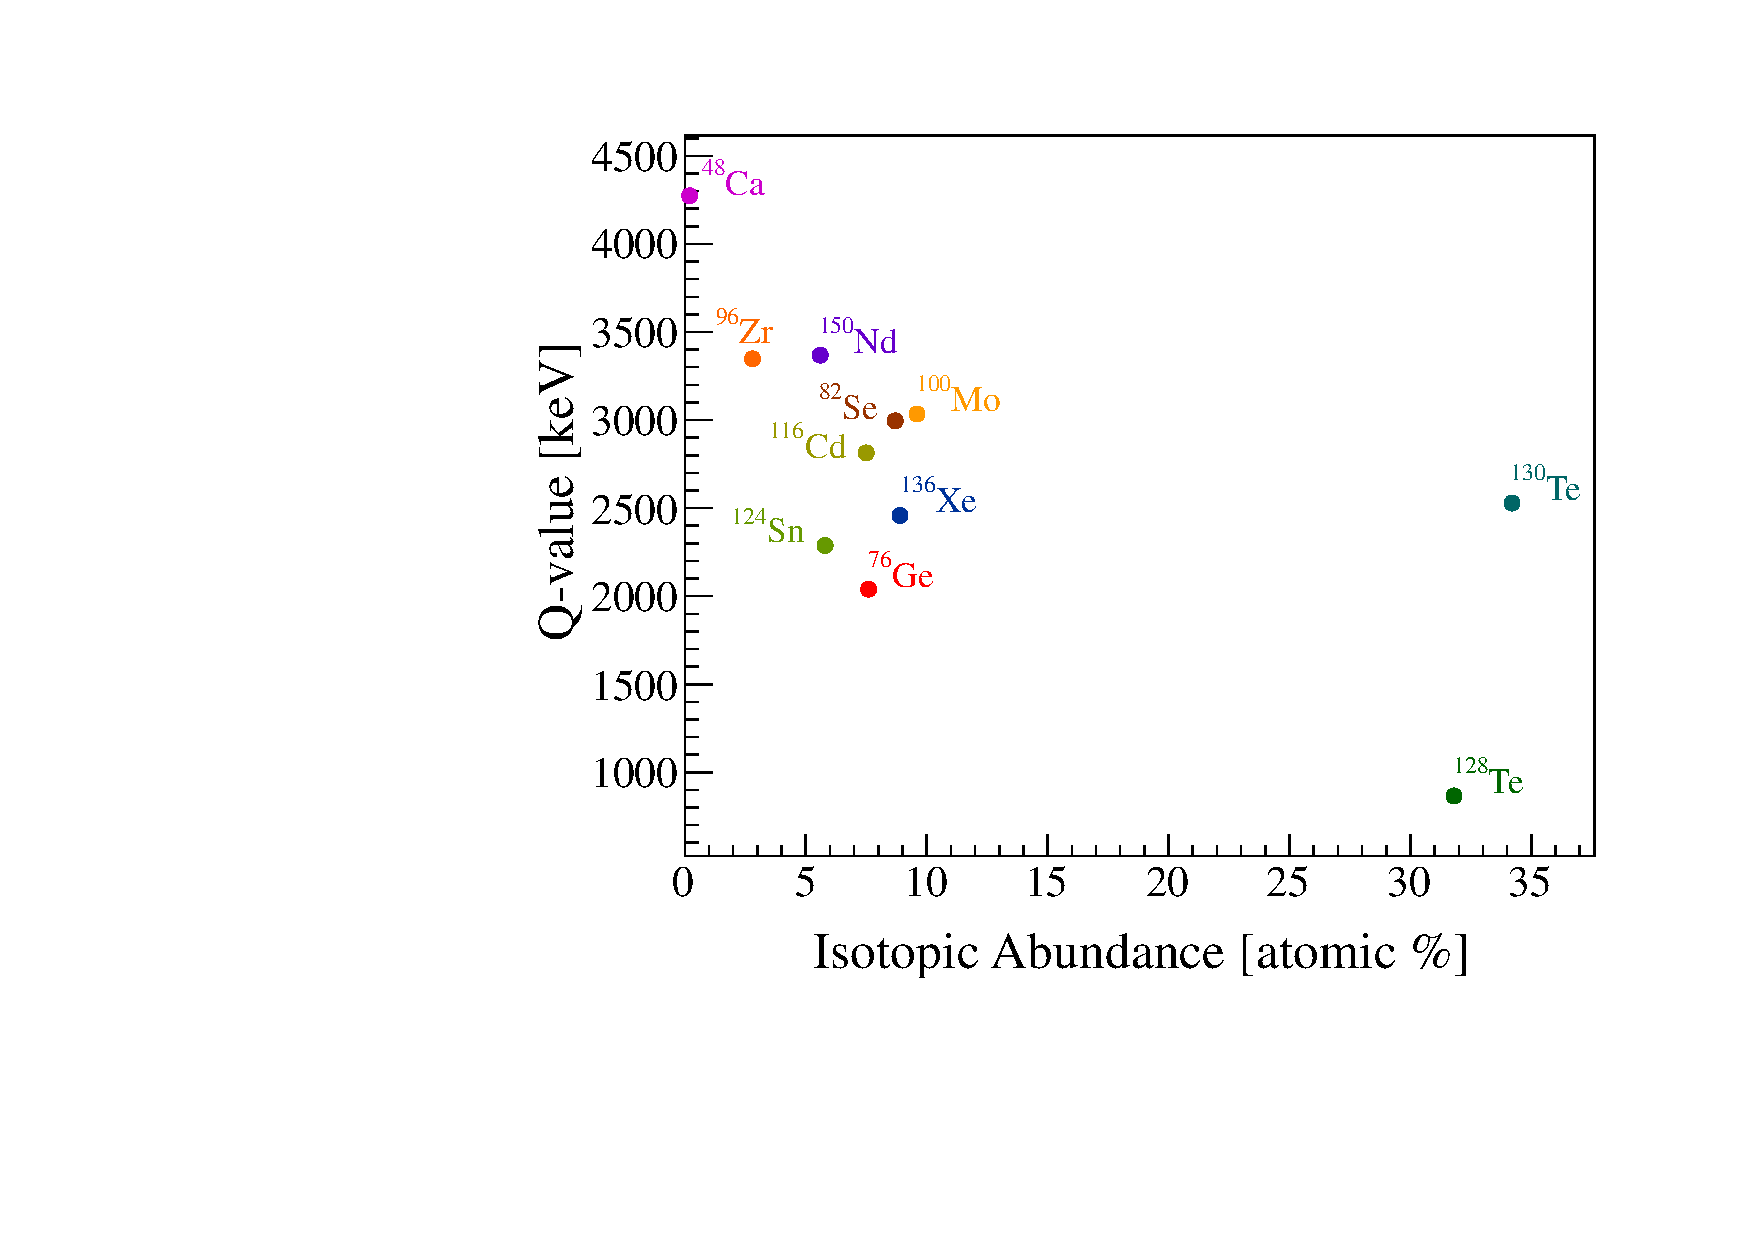
\includegraphics[width=0.7\linewidth]{Figures/q_vs_ia-color.pdf}
    \caption[The isotopic abundances and q-values of \zeronubb~candidate nuclei.]
    {The isotopic abundances and q-values of \zeronubb~candidate nuclei.
    Note that the \teonethirty~isotopic abundance is significantly higher for natural tellurium than for other elements.}
    \label{fig:q_vs_ia-color}
\end{figure}
A goal of many next-generation \zeronubb~decay experiments is to have a negligibly small background near the Q-value.
This changes the calculation in \autoref{eq:sensitivity_short} to be merely
\begin{align}
    S &\propto a_I \cdot M \cdot t
\end{align}
which is a significant increase in sensitivity, especially as experiments work to scale up in mass to become more sensitive to longer half-lives.
\subsection{Neutrinoless Double-Beta Decay with Majoron Emission}
\label{ssec:Neutrinoless Double-Beta Decay with Majoron Emisison}
\zeronubb~decays as shown in \autoref{eq:doubleneutrondecay} and \autoref{eq:doubleprotondecay} where only electrons are emitted are not the only possible decay mode for these candidate nuclei.
Some proposed models of \zeronubb~decay predict the existence of another particle, called a majoron, that is emitted during the decay.
In the original theory, these majorons are the Goldstone boson that is created during a spontaneous global breaking of B-L symmetry \cite{CHIKASHIGE1981265}.
The Majorons in the original models were posited as belonging to either a singlet, doublet, or triplet state, but the doublet and triplet states have been ruled out by precision measurements of the Z boson width at the LEP experiment \cite{ALEPH:2005ab}.
However, a whole class of models have now been developed that predict similar phenomena as the original theories where either one or two light, neutral bosons\footnote{Although the original majoron was postulated as a Goldstone boson, the majoron in these models may or may not be a Goldstone boson.}
are emitted during a neutrinoless double-beta decay \cite{HIRSCH19968}.
Decays emitting a single majoron are denoted as \zeronubbonechi, and decays emitting two majorons are denoted as \zeronubbtwochi.
These models are classified into two types (I and II) where either lepton number is (type I) violated in neutrinoless double-beta decay, i.e. the lepton number of the majoron is zero, or where lepton number is not (type II) violated, i.e. the lepton number of the majoron cancels out the $L=\pm2$ from the emitted electrons.
In models of type II, \zeronubb~decay without majoron emission is forbidden, whereas for models of type I, \zeronubb~decay is allowed.
However, as \zeronubb~decay has yet to be observed in the laboratory, these two types of models are indistinguishable from one another.
The types of models for majoron decay are summarized in \autoref{tab:Majoron Decay Modes}. 
\begin{table}[H]
    \centering
\begin{tabular}{lllcc}
\hline \hline
Model   & Decay Mode & Goldstone Boson & Lepton Number & Spectral Index \\ \hline
IB      & \zeronubbonechi & no              & 0    & 1              \\ 
IC      & \zeronubbonechi & yes             & 0    & 1              \\ 
ID      & \zeronubbtwochi & no              & 0    & 3              \\ 
IE      & \zeronubbtwochi & yes             & 0    & 3              \\ 
\hline
IIB     & \zeronubbonechi & no              & -2   & 1              \\ 
IIC     & \zeronubbonechi & yes             & -2   & 3              \\ 
IID     & \zeronubbtwochi & no              & -1   & 3              \\ 
IIE     & \zeronubbtwochi & no              & -1   & 7              \\ 
IIF     & \zeronubbonechi & no              & -2   & 3              \\ 
\hline
``bulk" \cite{Mohapatra:2000px} & \zeronubbonechi & no              & 0    & 2              \\
\hline \hline
\end{tabular}
\caption[The majoron models and their associated decay modes.]
{The majoron models and their associated decay modes.
Also shown is if the majoron is a Goldstone boson, the associated lepton number of the majoron, and the spectral index of the decay.
In models of type II \zeronubbtwochi, each majoron has an associated lepton number which precisely cancels out the $\Delta L$ carried by the electrons in these \zeronubbtwochi~decays.}
\label{tab:Majoron Decay Modes}
\end{table}
Experimentally, the energy spectrum of the two electrons emitted varies by the spectral index of each of the models according to
\begin{align}
    S(E_{\textrm{sum}}) &= \int_1^{E_{sum}-1}F(Z, E_1) E_1 p_1 F(Z, E_2) E_2 p_2 (E_{tot}-E_1-E_2)^n dE_1 dE_2 \delta(E_{sum}-E_1-E_2)
    \label{eq:spectral index}
\end{align}
where $E_{\textrm{sum}}$ is the summed energy of the electrons, $F(Z, E)$ is the Fermi function for the daughter nucleus with atomic number Z, $E_i$ and $p_i$ are the energy and momentum of each particle, respectively, and $n$ is the spectral index.
The Fermi function comes from a correction due to Coulomb interactions between the emitted electrons and the daughter nucleus in the decay.
To lowest order, this function is given by 
\begin{align}
    F(Z,E) &= 4(2 p \rho)^{2(\gamma - 1)}e^{y\pi} \frac{|\Gamma(\gamma+iy)|^2}{|\Gamma(2\gamma+1)|^2}\frac{1+\gamma}{2} \\
    \gamma &= (1-(\alpha Z)^2)^{1/2} \\
    y &= \alpha Z W / p
\end{align}
where $\rho$ is the nuclear radius, $p$ is the momentum of the electron, and $\Gamma(x)$ is the gamma function\footnote{$\Gamma(z)=\int_0^\infty x^{z-1}e^{-x}dx$} \cite{PhysRev.150.846}.
The spectrum for \twonubb~decay corresponds to a spectral index of 5.
The energy spectrum for each spectral index of \zeronubb~with majoron emission is shown in \autoref{fig:Majoron Spectrum}.

\begin{figure}[htbp]
    \centering
    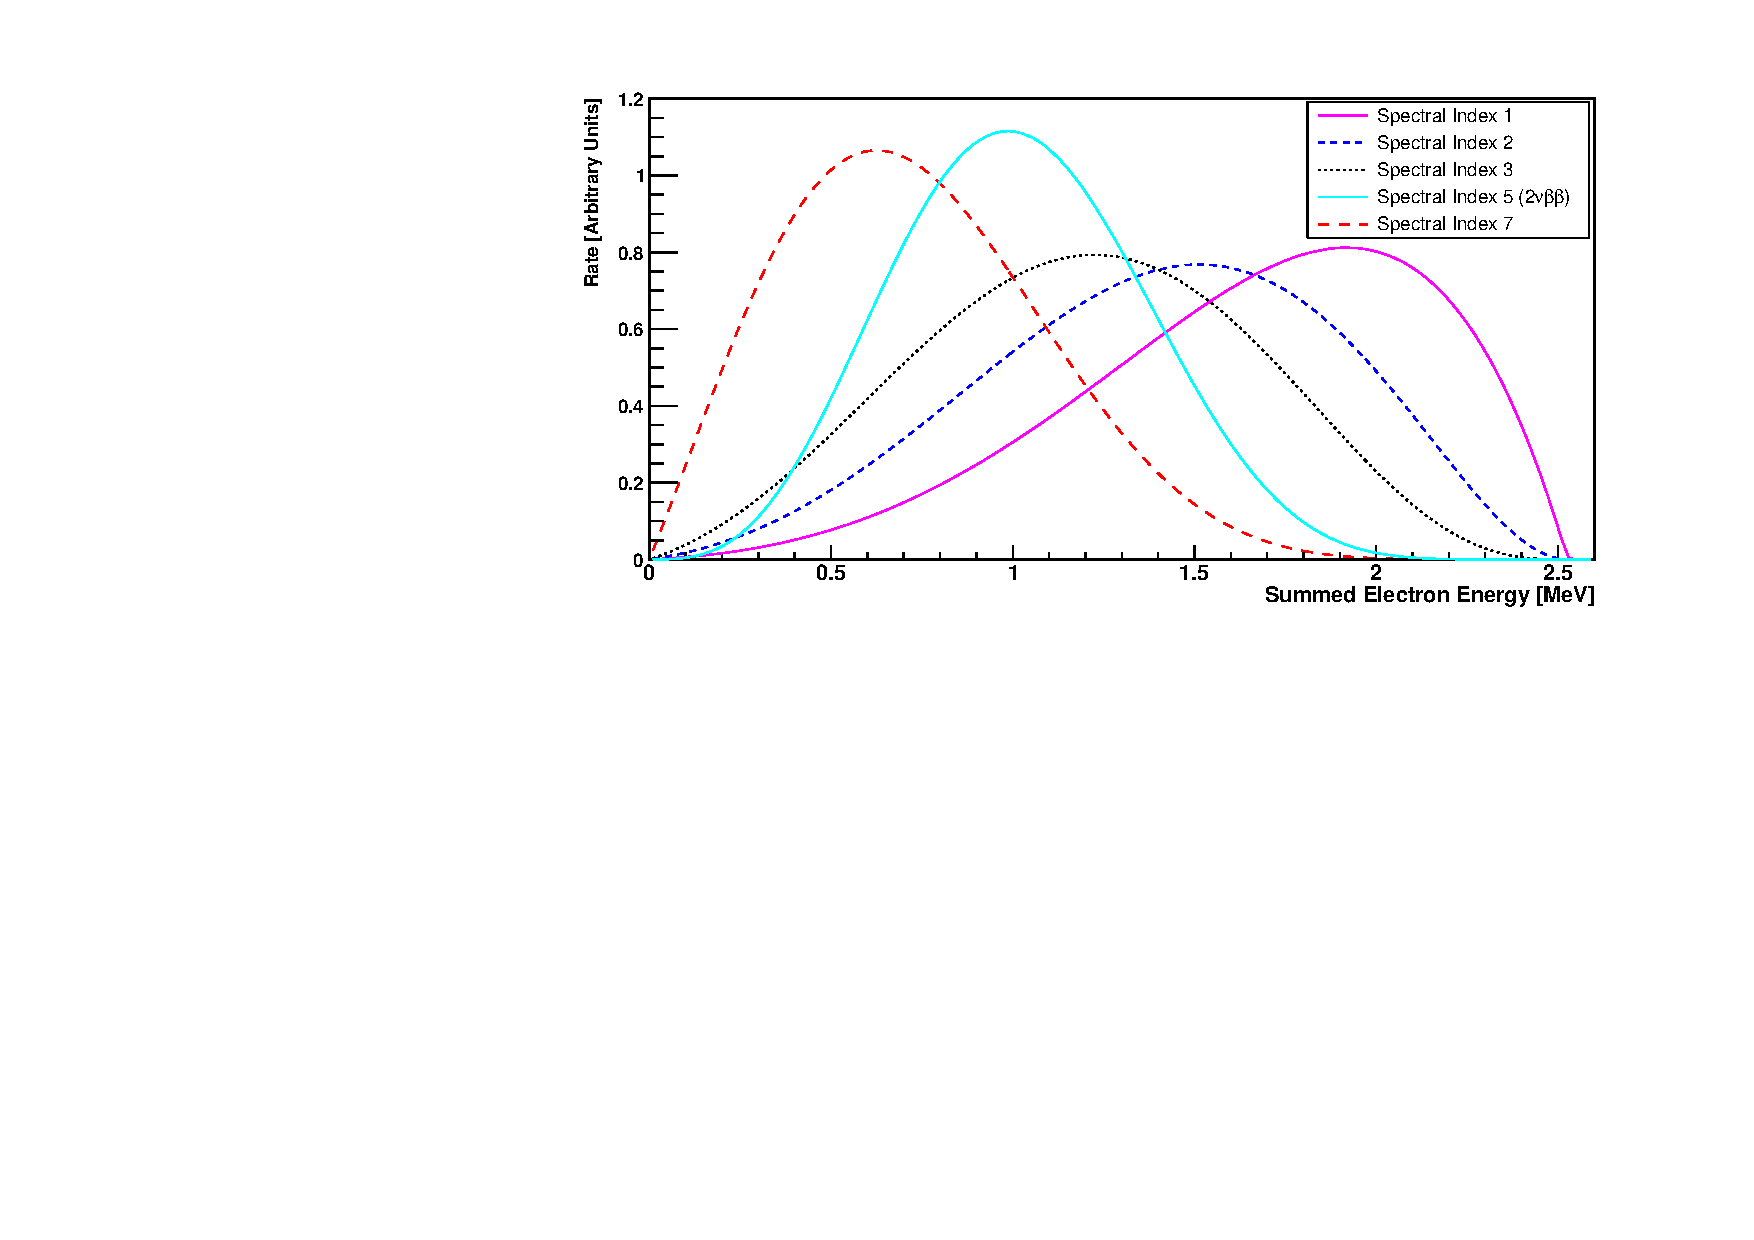
\includegraphics[width=0.9\linewidth]{Figures/EnergySpectrum_fixedFermi.pdf}
    \caption[The summed electron energy spectra for multiple types of Majoron emission according to spectral indices 1, 2, 3, 5, and 7.]
    {The summed electron energy spectra for multiple types of Majoron emission according to spectral indices 1, 2, 3, 5, and 7.
    Spectral index 5 corresponds to \twonubb~and is not a Majoron decay, but is shown for context.
    The integrals of each of the spectra are normalized to 1.}
    \label{fig:Majoron Spectrum}
\end{figure}

\section{State of Neutrinoless Double-Beta Decay Experiments}
\label{sec:State of Neutrinoless Double Beta Decay Experiments}
In addition to CUORE, many other experiments are currently searching and have searched for \zeronubb~ decay. Some of these experiments are listed below and the current status of the field is shown in \autoref{fig:cuore-mbetabeta}.
As noted before in \autoref{sec:Double Beta Decay} and \autoref{sec:Neutrinoless Double Beta Decay}, the signatures of \zeronubb~ and \twonubb~ decays are a nucleus that interchanges two neutrons and two protons, along with the emission of two electrons and, in the case of \twonubb~decay or Majoron emission, two neutrinos and up to two Majorons.
Since the half-lives of these decays are so large, (consider that the Universe is only $1.38\times10^{9}~\textrm{yr}$ old) an experiment needs to have extremely low background levels in order to be able to even observe these events.
As an example, a 1-tonne experiment searching for \zeronubb~decay would expect only $\mathcal{O}(10)$ events per year.
This is generally realized in experiments by going to deep underground laboratories to escape cosmic radiation sources and by having pure and clean materials in and near the detector and sources.
Also, due to the energies being produced according to a spectrum, all of the backgrounds with energy up to the Q-value will reduce the sensitivity of the measurement.
The experiments listed here all seek to identify these signals using a particular technology or set of technologies, some of which, especially in the case of GERDA and MAJORANA, are quite similar to CUORE's.
Despite the wide array of technologies, all the experiments below, including CUORE, seek to identify these decays by honing in on and measuring the emitted electron energies as the summed energy spectrum is well-defined as a sharp peak for \zeronubb~or as a broader spectrum for \twonubb~for Majoron emission.

\begin{figure}[htbp]
\centering
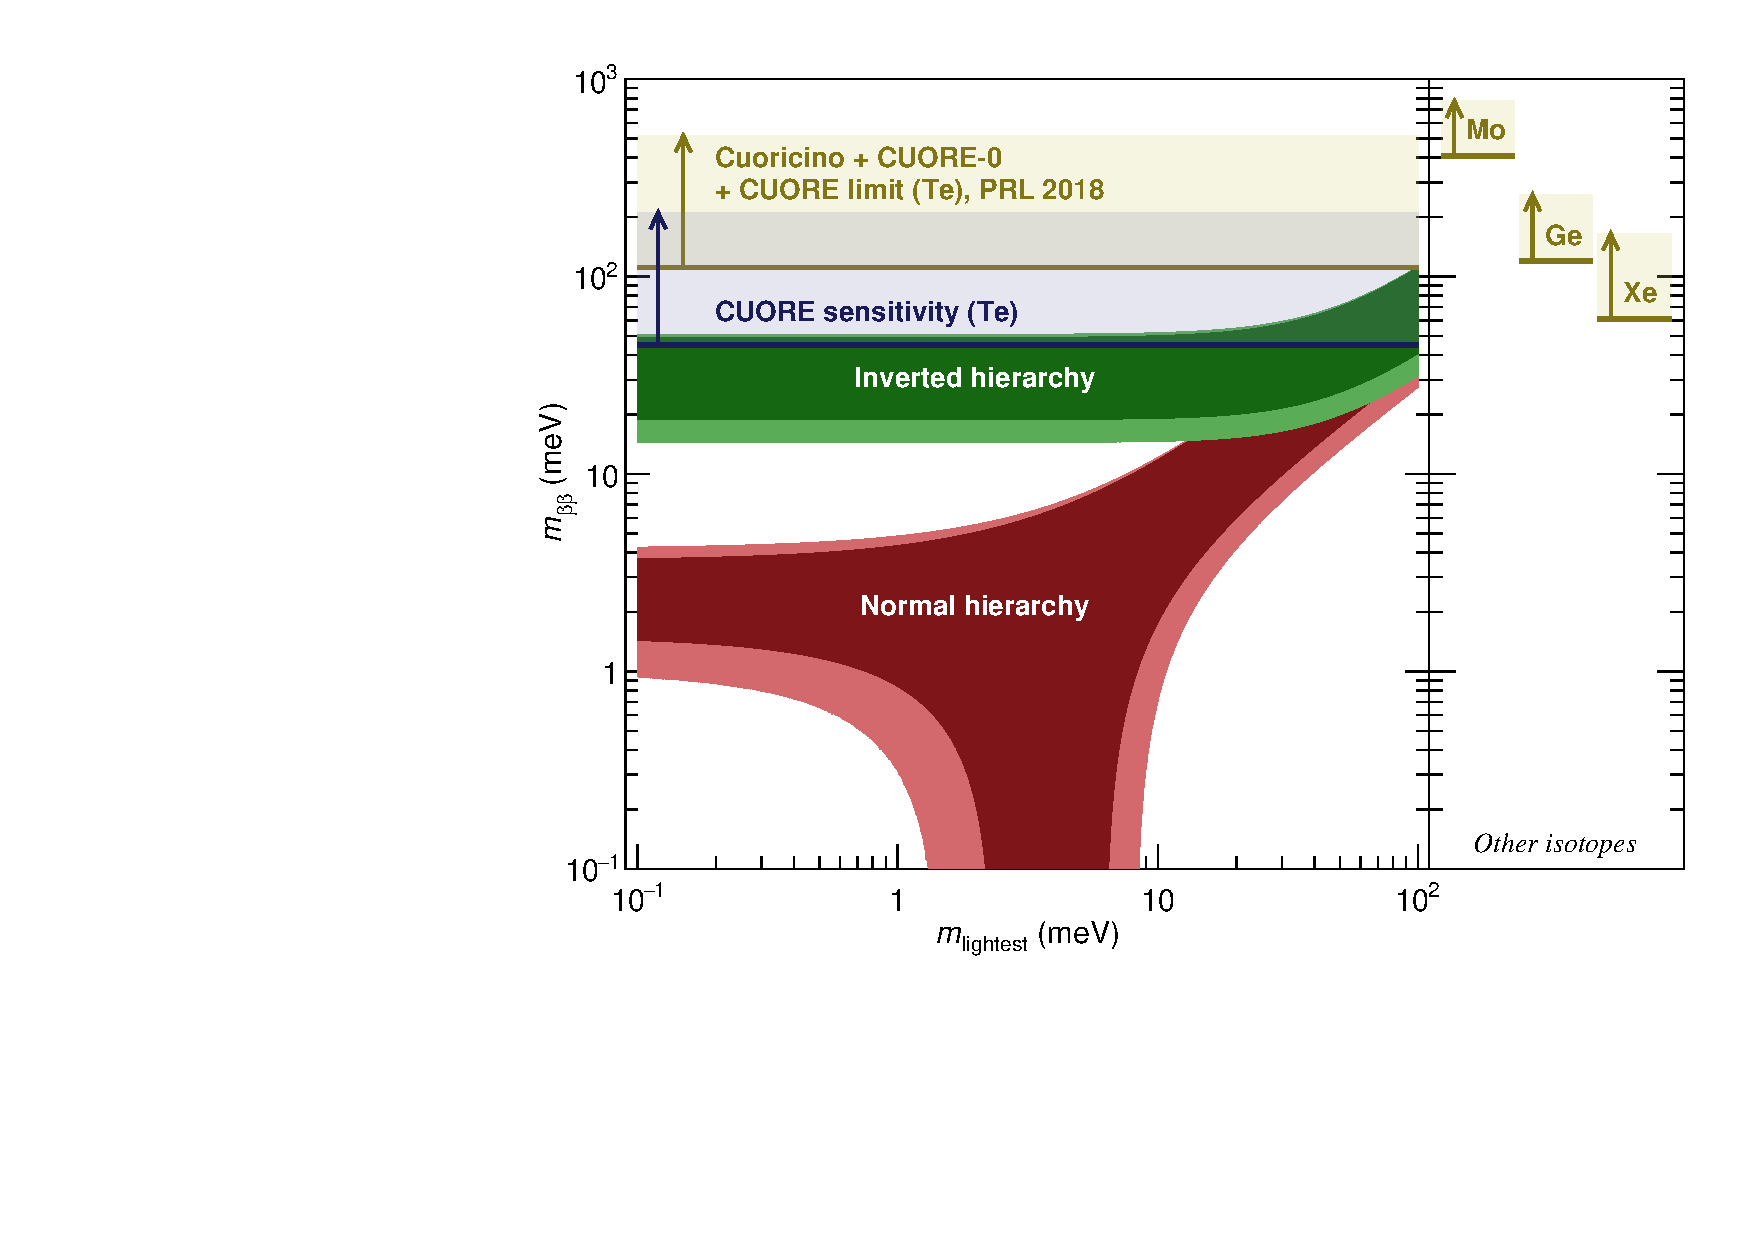
\includegraphics[width=0.7\linewidth]{Figures/M_bb_vs_mlightest_CL_2018.pdf}
\caption[The current status of the field of \zeronubb.]
{The current status of the field of \zeronubb. See \autoref{eq:mbetabeta} for the definition of $m_{\beta\beta}$ and $m_{\textrm{lightest}}$ corresponds to the mass of the lightest neutrino in either normal or inverted hierarchy.
The previous experiments in the line of CUORE, CUORE-0 and Cuoricino, have their combined $^{130}$Te result and the results for Mo, Ge, and Xe are shown from NEMO-3, GERDA, and KamLAND-Zen, respectively.}
\label{fig:cuore-mbetabeta}
\end{figure}

\subsection{GERDA}

The GERmanium Detector Array (GERDA) Experiment is currently searching for \zeronubb~at the Laboratori Nationali del Gran Sasso (LNGS) using  $^{76}$Ge as the source \cite{Agostini:2017iyd}.
Unlike in CUORE, the source is enriched from the natural $7.8\%$ abundance up to $86\%$ and acts acts both the source and the detector of \zeronubb.
In the most recent phase of GERDA, Phase II, 37 enriched detectors, 35.6 kg, are assembled along 6 strings around a central string with 3 unenriched detectors.
These detectors are then submerged in a 64 $\textrm{m}^3$ LAr cryostat inside a 590 $\textrm{m}^3$ water tank.
The water acts as a passive shield for the experiment, while the LAr also acts as an active shield.
One of the advantages that CUORE shares with GERDA over other detector technologies is the excellent energy resolution which, recalling \autoref{eq:sensitivity_short} inversely effects the sensitivity.
GERDA also takes advantage of the pulse-shape discrimination (PSD) between \zeronubb-like events and $\gamma$-like events in 30 broad energy (BEGe) detectors in addition to scintillation light from the surrounding LAr.
With this, the background at $Q_{\beta\beta}$ for the BEGe detectors is low enough at $(0.07^{+1.1}_{-0.5})\times 10^{-3} ~\textrm{counts} \cdot  (\textrm{keV} \cdot \textrm{kg} \cdot \textrm{yr})^{-1}$ allowing for the experiment to be considered background-free at the design exposure of $100 \textrm{kg \cdot yr}$.
A diagram of the GERDA experimental setup is shown in \autoref{fig:gerda-labelled}.
\begin{figure}[tbph]
\centering
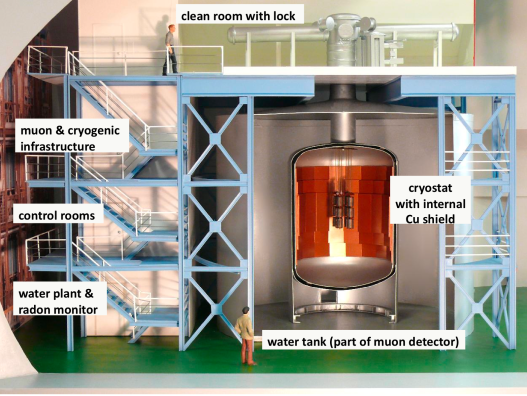
\includegraphics[width=0.7\linewidth]{Figures/gerda-view.png}
\caption[Diagram of the GERDA detector.]
{Diagram of the GERDA detector.
Liquid argon is also inside the copper shielding with the detectors submerged.}
\label{fig:gerda-labelled}
\end{figure}

\subsection{MAJORANA}
The \textsc{Majorana Demonstrator}, shown in \autoref{fig:MajoranaDemonstrator} is another experiment using $^{76}$Ge to search for \zeronubb~located in the Sanford Underground Research Facility in South Dakota.
This experiment deploys 30 kg of Ge enriched to 87\% $^{76}$Ge and 14 kg of Ge with natural 7.8\% $^{76}$Ge \cite{1742-6596-606-1-012004}.
The detection principles for the \textsc{Demonstrator} are similar to that of GERDA, but there are differences in detector operation and construction, particularly as the \textsc{Demonstrator} does not have the active lAr veto from GERDA, but has a more stringent materials selection and parts processing which results in their background rate of $1.6^{+1.2}_{-1.0}\times10^{-3} ~\textrm{counts}\cdot(\textrm{keV}\cdot \textrm{kg} \cdot \textrm{yr})^{-1}$.
\begin{figure}
    \centering
    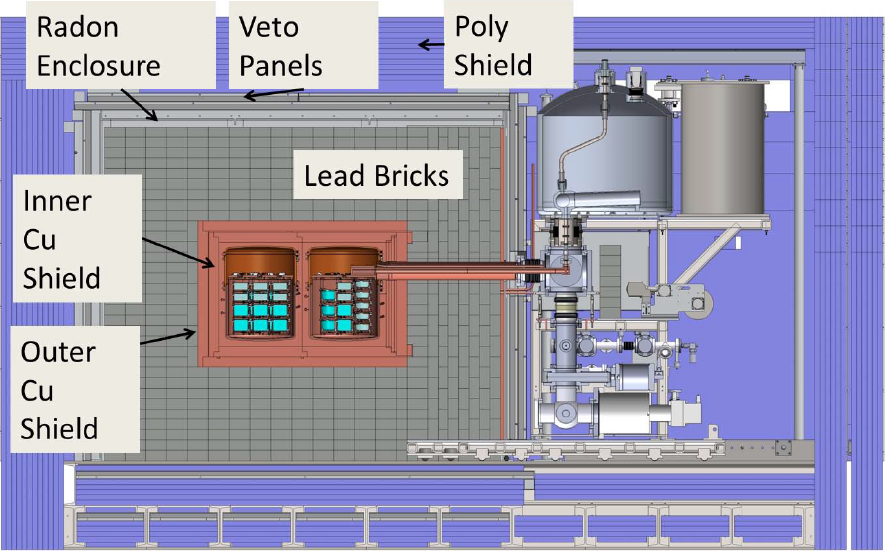
\includegraphics[width=0.8\linewidth]{Figures/MajoranaDemonstrator.png}
    \caption[The \textsc{Majorana Demonstrator} experimental apparatus.]
    {The \textsc{Majorana Demonstrator} experimental apparatus.
    The external active and passive shielding is shown enclosing the detectors inside the two cryostats.
    Figure from \cite{1742-6596-606-1-012004}.}
    \label{fig:MajoranaDemonstrator}
\end{figure}
\subsection{KamLAND-Zen}
The Kamioka Liquid Scintillator Antineutrino Detector Zero-neutrino double-beta decay search (KamLAND-Zen) searches for \zeronubb~in 90.8\% enriched $^{136}$Xe \cite{KamLAND-Zen:2016pfg}.
This experiment uses the existing infrastructure from the KamLAND experiment, with a balloon filled with enriched Xe in the center of the KamLAND liquid scintillator.
The detector uses the Xe-doped (2.9\% by weight) liquid scintillator acting as both the source and detector of \zeronubb.
Xe benefits from self-shielding due to the attenuation length of gammas in xenon which allows for reduced levels of background in the innermost volume.
This is a distinct advantage over experiments such as CUORE, MAJORANA, and GERDA, as their detectors need to be held in place and cannot self-shield as a result.
Also, the detector mass is relatively easily scalable by the size of the balloon and does not require a full reconstruction of the surrounding veto from the KamLAND experiment.
In addition, by taking out the Xe or depleting the Xe in the liquid scintillator, the experiment can make an on/off measurement to confirm any possible measurement of \zeronubb. 
However, the energy resolution of the KamLAND-Zen is significantly worse than the $\mathcal{O}(\textrm{keV})$ resolution in these experiments which introduces the tail of the \twonubb spectrum as an irreducible background.
A diagram of the KamLAND-Zen detector is shown in \autoref{fig:kamlandzen}.
\begin{figure}[tbph]
\centering
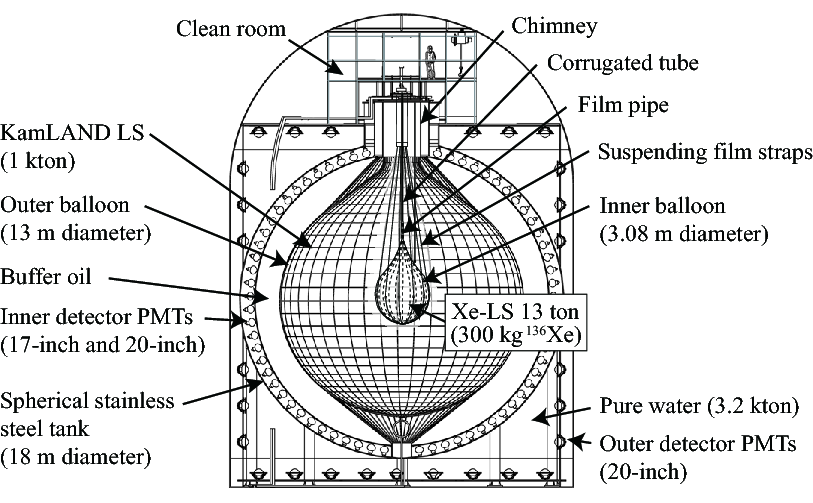
\includegraphics[width=0.7\linewidth]{Figures/KamlandZen}
\caption[A schematic of the Kamland-Zen experimental apparatus.]
{A schematic of the Kamland-Zen experimental apparatus.
The Xe-loaded liquid scintillator is held within the balloon at the center.
Figure from \cite{::2015uaa}.}
\label{fig:kamlandzen}
\end{figure}

\subsection{EXO-200}
The Enriched Xenon Observatory (EXO-200) searches for \zeronubb~ with 200 kg of Xe with 80.6\% enriched $^{136}$ Xe in a liquid xenon time projection chamber (TPC) and is located in the Waste Isolation Pilot Plant near Calsbad New Mexico \cite{Albert:2017owj}.
The TPC collects both charge and light signals from energy depositions in the Xe and reconstructs them as either single-site or multi-site events.
This provides discrimination between the multi-site \gamma~backgrounds and the single-site signal.
\begin{figure}[htbp]
    \centering
    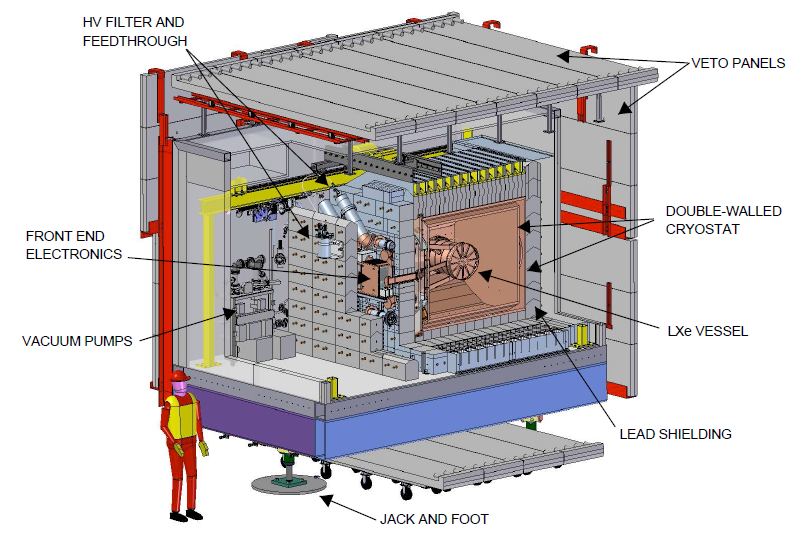
\includegraphics[width=0.7\linewidth]{Figures/EXO.png}
    \caption[The EXO-200 detector setup.]
    {The EXO-200 detector setup.
    The LXe TPC is contained within the cryostat, with the entire setup surrounded by a muon veto.
    Figure from \cite{Auger:2012gs}.}
    \label{fig:EXO}
\end{figure}

\subsection{NEMO-3}
The Neutrino Ettore Majorana Observatory (NEMO-3) collected \twonubb~data from multiple isotopes including $^{100}$Mo, $^{82}$Se, $^{130}$Te, $^{116}$Cd, $^{150}$Nd, $^{96}$Zr, and $^{48}$Ca \cite{Bongrand:2011ei}.
NEMO-3 also searched for \zeronubb~in $^{100}$Mo, $^{82}$Se, $^{48}$Ca, and $^{150}$Nd \cite{Bongrand:2011ei}\cite{Arnold:2016qyg}\cite{Arnold:2016ezh}.
Unlike the other experiments listed in this section, NEMO-3 did not utilize a ``detector = source" method, instead using separate detectors and sources.
An advantage of this method is that the two emitted electrons can be tracked and measured separately, which is a clear signal that a decay occured as a vertex can be reconstructed along with the energies of the particles.
An example track in NEMO-3 is shown in \autoref{fig:nemo3393042373top2}.
Another advantage is that the source foil can be easily replaced with other isotopes while leaving the rest of the detector apparatus unchanged.
However, this is a constraint on the size of the source, as it needs to be small enough for electrons to traverse and be detected outside, yet, as shown in \autoref{eq:sensitivity_short}, the number of decays scales with the source mass.
\begin{figure}[htbp]
\centering
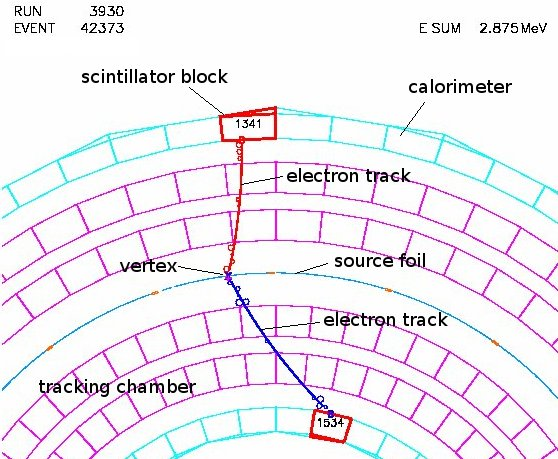
\includegraphics[width=0.7\linewidth]{Figures/nemo3_3930_42373_top_2}
\caption[An example double-beta decay candidate event from NEMO-3.]{An example double-beta decay candidate event from NEMO-3.
The electrons are emitted from a nucleus in the source foil and deposit energy in the calorimeter after leaving tracks in the tracking chamber.}
\label{fig:nemo3393042373top2}
\end{figure}

\chapter{CUORE}
\label{ch:CUORE}
CUORE (Cryogenic Underground Observatory for Rare Events) is located in Gran Sasso, Italy, and utilizes a bolometric method to search for \zeronubb. The experiment will run with 988 crystals of TeO$_2$ held at roughly 10 mK.
The source of \zeronubb~are the $^{130}$Te nuclei inside of the crystals ($34.2\%$ natural abundance \cite{Fehr200483}).
Thus, in this setup, the crystals act as both sources and detectors of \zeronubb. When energy is deposited in the crystals, such as from the electrons emitted during \zeronubb, the temperature of the crystals rises.
The Q-value of the decay of interest, viz. $^{130}\textrm{Te} \rightarrow ^{130}\textrm{Xe} + e + e$, is $2527.518\pm 0.013$ keV \cite{Redshaw:2009cf, Scielzo:2009nh, Rahaman:2011zz}.
This high Q-value is well-separated from other naturally occurring environmental $\gamma$'s except for $^{60}$Co at 2506 keV and $^{208}$Tl at 2615 keV.
However, the resolution of the CUORE crystals is $7.7\pm0.5$ keV, which means that these peaks do not significantly worsen the background in the region of interest at the Q-value.
In addition, this resolution aids in understanding background sources that deposit energy the detector as each \gamma~line can be observed above the Compton background, which aids in identifying particular background sources.

\section{CUORE Detectors}

\subsection{Particle Detection with Bolometers}
\label{ssec:Particle Detection with Bolometers}
As noted in \autoref{sec:State of Neutrinoless Double Beta Decay Experiments}, current experiments in the field of \zeronubb~use a wide array of technologies to identify \zeronubb~events.
However, CUORE utilizes a different method of calorimetry than its counterparts in that it uses a technique known as the bolometric method, which was first proposed for use in \zeronubb~experiments by Ettore Fiorini and Tapio Niinikosky \cite{FIORINI198483}.
As particles pass through matter, the energy they deposit is eventually carried into the surrounding material as heat.
This method requires a mass that acts as a thermal capacitor, a weak thermal connection to a heat bath, and a thermometer (generally a thermistor) and CUORE's setup is sketched in \autoref{fig:thermal_crystal_cartoon} and a sample pulse is shown in \autoref{fig:Sample_pulse}.
The detectors in CUORE, $\textrm{TeO}_2$~crystals, respond to energy deposition by a temperature rise according to
\begin{equation}
\delta T = \delta E/C(T).
\end{equation}
At low C, $\delta T$ is maximized; therefore, the crystals are operated at low temperatures where C(T) is given by the Debye Model:
\begin{equation}
C(T)\sim (\frac{T}{\Theta_D})^3
\end{equation} 
where $\Theta_D$ is the Debye temperature for \teotwo, $232\pm7~\textrm{K}$ \cite{BolometerCalculations}. This strong temperature dependence on the heat capacity is what drives the need for low temperatures in CUORE, where we have achieved an operational temperature of $\sim10$ mK.
The custom cryostat used to do this is described later on in \autoref{sec:CUORE Cryostat}.
At these temperatures, a 1 MeV energy deposit in a single CUORE crystal would cause the temperature to rise to $\sim 100~\textrm{\mu K}$. 

\begin{figure}[htbp]
\centering
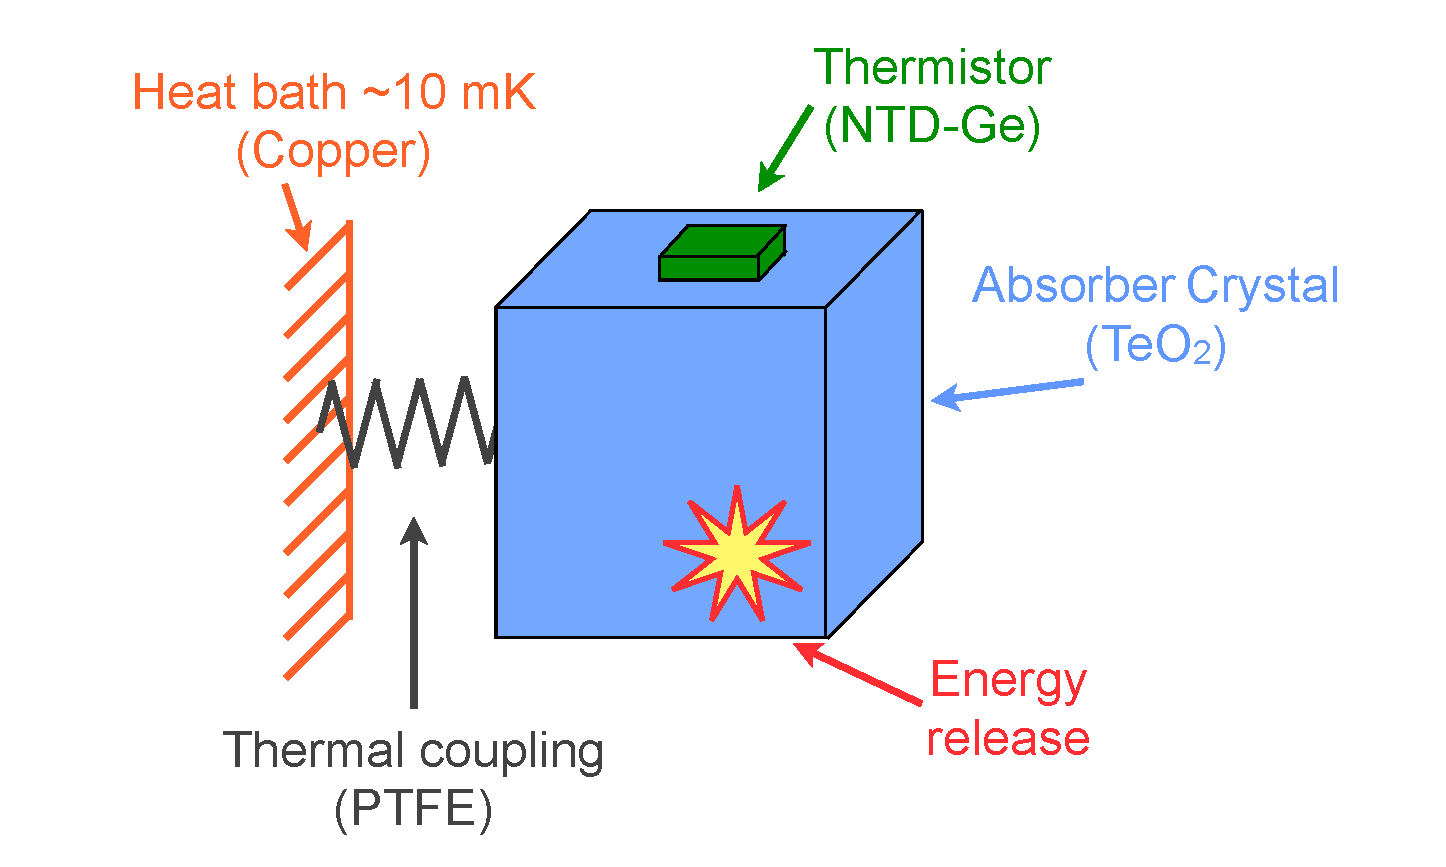
\includegraphics[width=0.7\linewidth]{Figures/bolosketch-color.pdf}
\caption[A diagram of the thermal connection of the TeO$_2$ crystals to the thermal bath provided by the copper frames.]
{A diagram (not to scale) of the thermal connection of the TeO$_2$ crystals to the thermal bath provided by the copper frames.
The weak thermal coupling is provided by the PTFE.}
\label{fig:thermal_crystal_cartoon}
\end{figure}

\subsubsection*{Bolometer Thermometry Instrumentation}
Of course, an integral component to the bolometric method is the choice of thermometer used to detect these changes in temperature.
The choice of thermometer that CUORE uses is a Neutron Transmutation Doped (NTD) germanium thermistor due to its reproducibility and uniformity, which is critically important across CUORE's crystal array. However, a drawback to this is that each NTD thermistor must be individually cut from a block and then mounted onto each bolometer \cite{NTDThermistor}.

\begin{figure}[htbp]
%\captionsetup[subfigure]{justification=centering}
\centering
\begin{subfigure}[t]{0.40\textwidth}
\centering
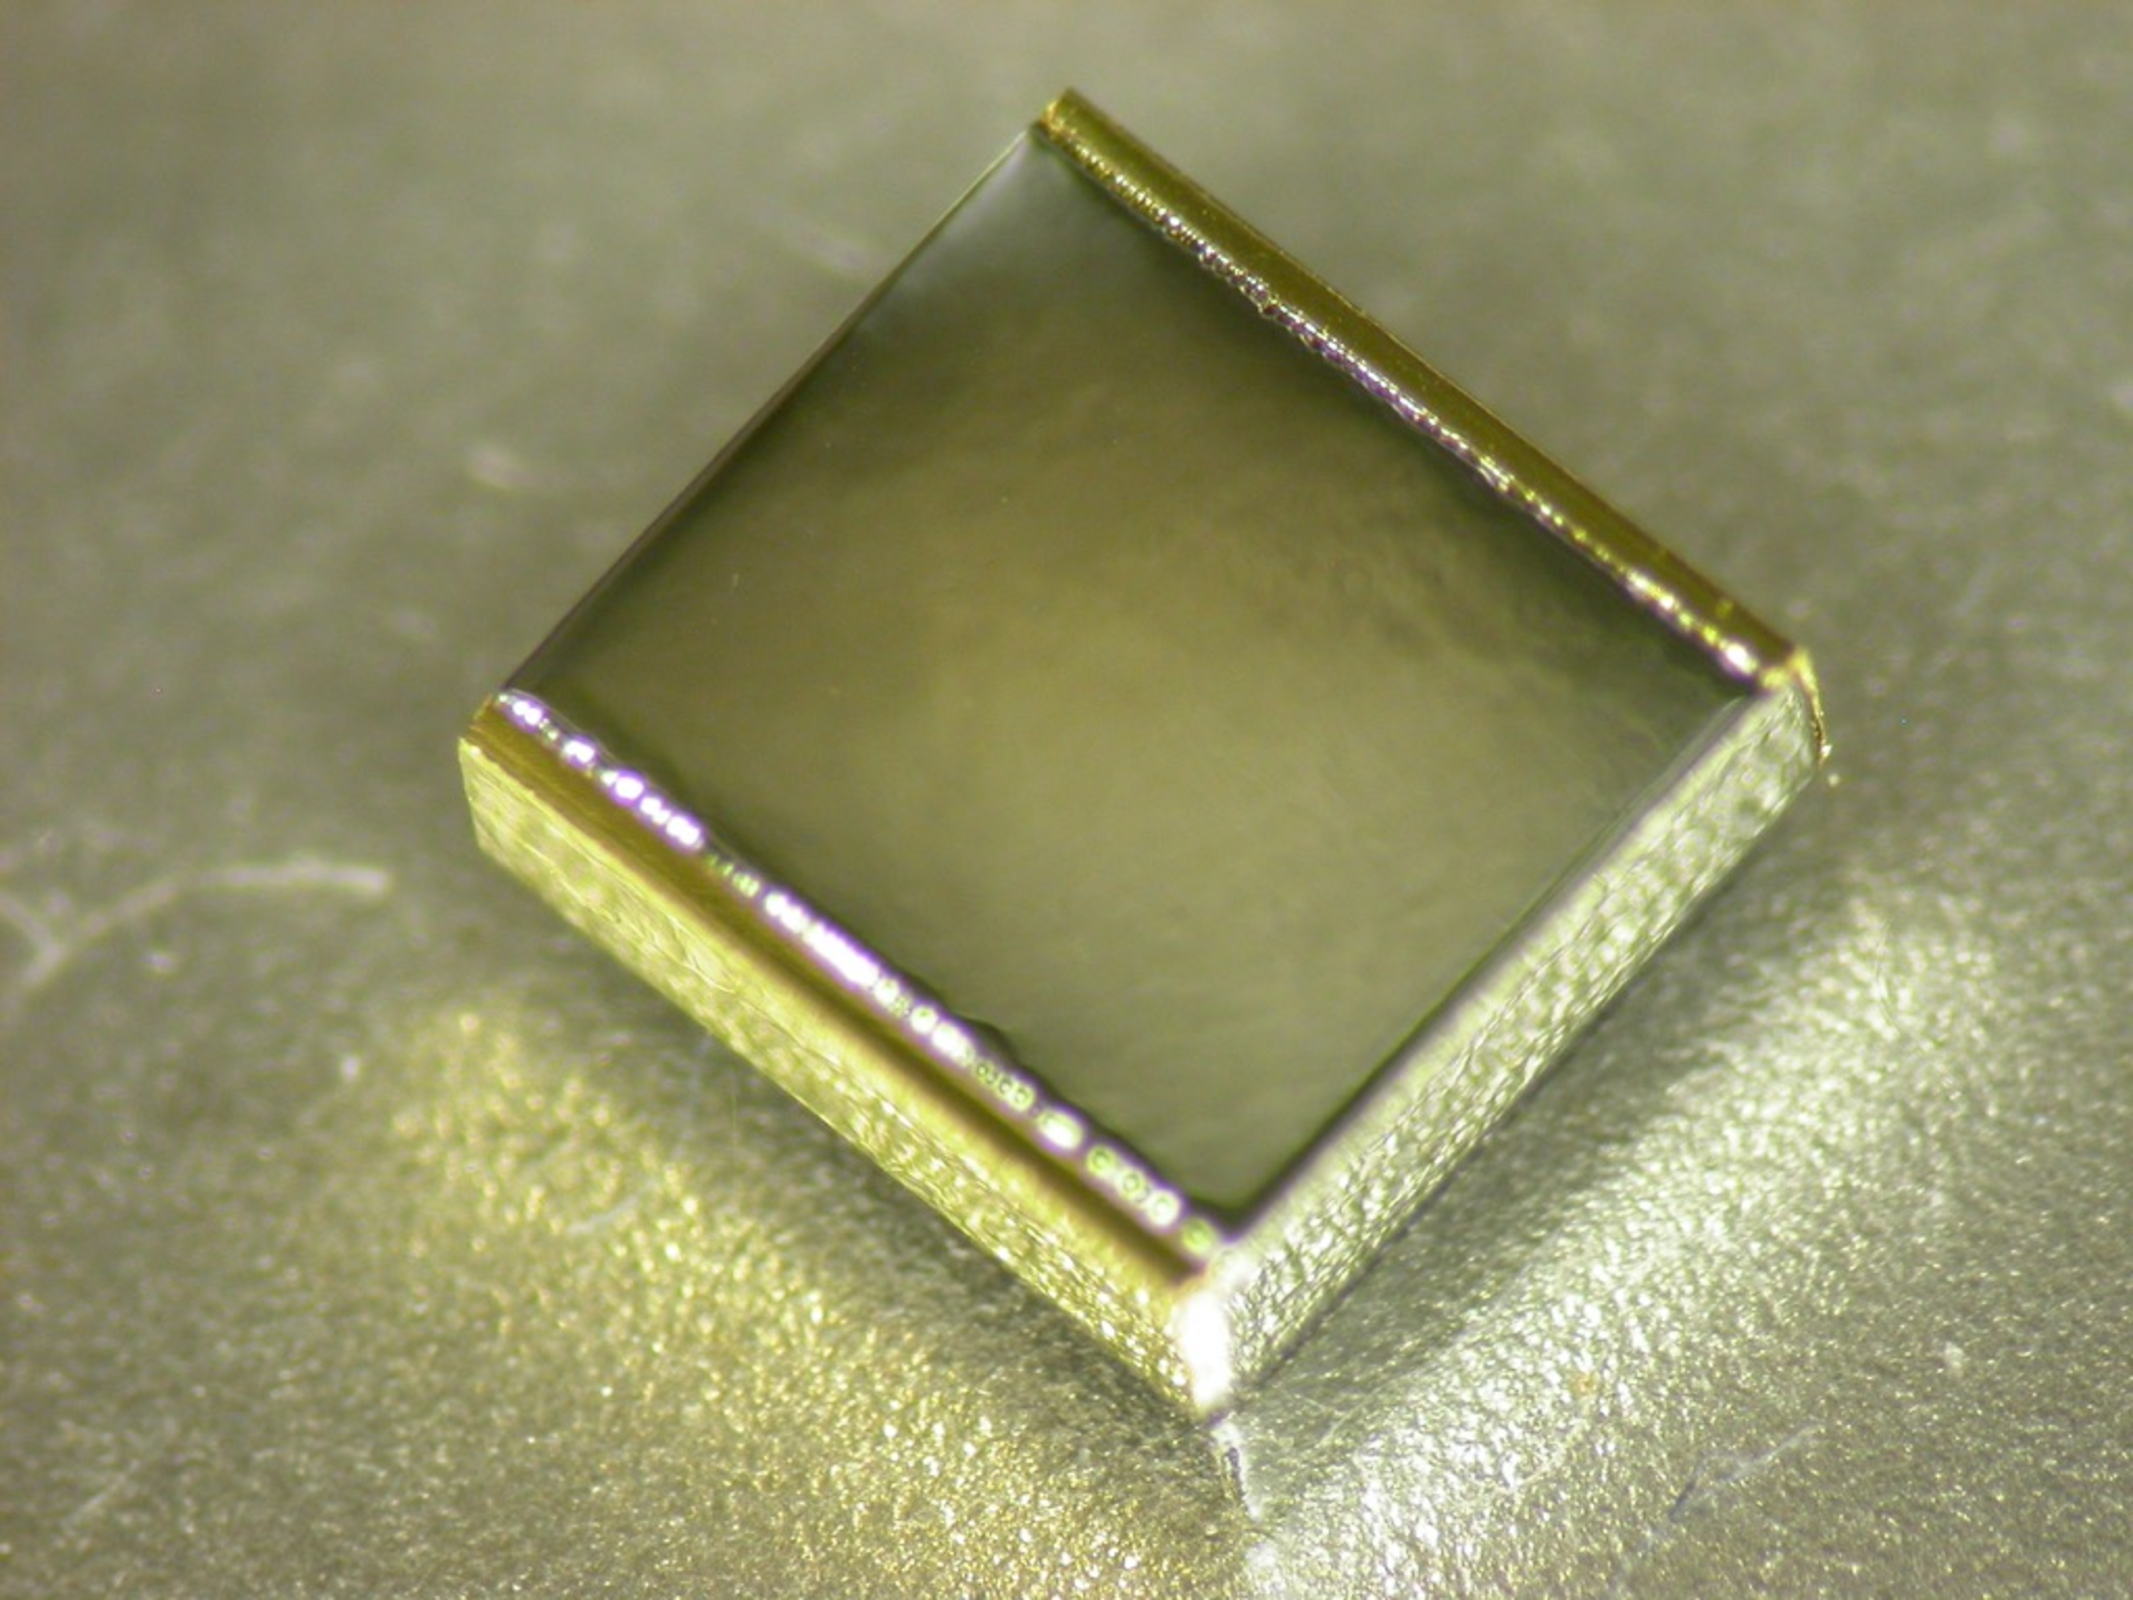
\includegraphics[width=0.9\textwidth]{Figures/fig04a.pdf}
\caption{}
\label{fig:NTD_picture}
\end{subfigure}
\qquad
\begin{subfigure}[t]{0.40\textwidth}
\centering
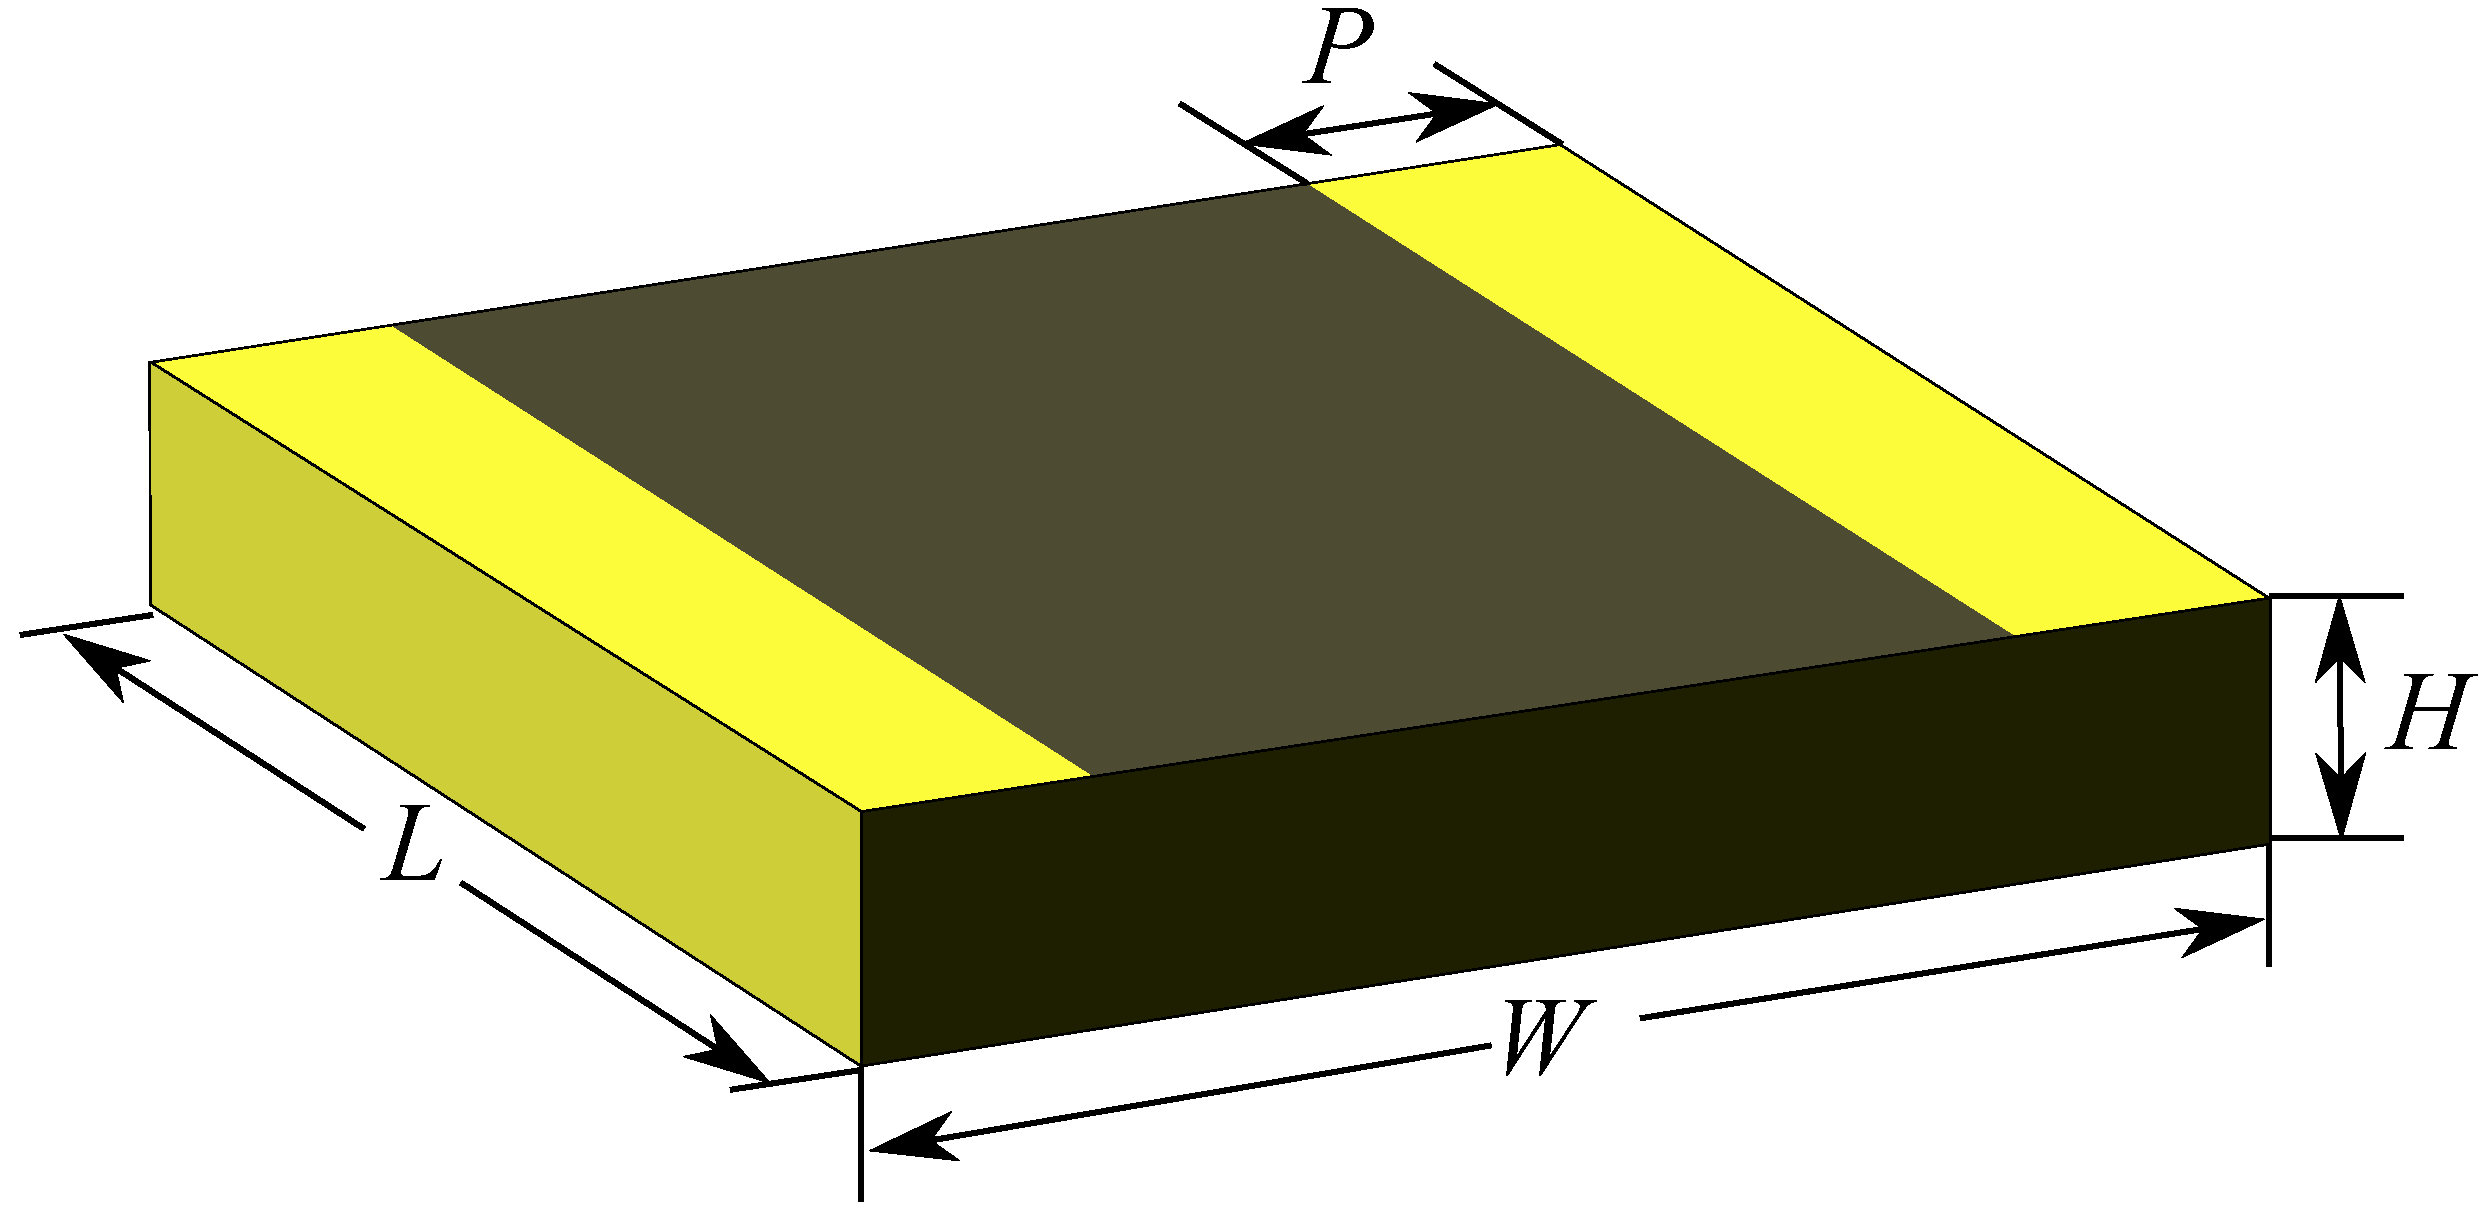
\includegraphics[width=0.9\textwidth]{Figures/fig04b.pdf}
\caption{}
\label{fig:NTD_sketch}
\end{subfigure}
\caption[A photograph (a) and a diagram (b) of an NTD thermistor used in CUORE.]
{A photograph (a) and a diagram (b) of an NTD thermistor used in CUORE.
The dimensions of the NTD are $3.0\times2.9\times0.9~\textrm{mm}^3$ ($\textrm{L} \times \textrm{W} \times \textrm{H}$ with $\textrm{P}=0.2~\textrm{mm}$.
Figure from \cite{Alduino:2016vjd}.}
\label{fig:NTD}
\end{figure}

The NTD thermistors are created by irradiating pure Ge with a flux of thermal neutrons, and the NTD sensors used in CUORE were irradiated at the MIT Nuclear Reactor Laboratory.
This flux produces Ga, As, and Se, which dopes the Ge, and the doping stops before the Ge reaches a critical doping threshold such that it still remains a semiconductor.
Above this threshold, the Ge material acts as a metal where resistivity goes to 0 at 0 K, but just below this threshold, the resistivity increases sharply.
This is due to the fact that the doping causes conduction electrons in the material to localize into the doped atoms which are spread out into the germanium.
When conducting at high temperatures, the electrons tunnel to the nearest available unoccupied sites in the material.
At low temperatures, however, such as the $<1~\textrm{K}$ temperatures of the CUORE detectors, the resulting lack of higher-energy phonons prevents the electron from tunneling into the nearest sites, and instead favor sites with similar energies to the electron.
In this regime of ``variable range hopping", the resistance of the NTD goes as
\begin{equation}
    R(T) = R_0 e^{\left(\frac{T_0}{T}\right)^p} 
    \label{eq:NTD_Resistivity}
\end{equation}
as shown by Shklovskii and Efros \cite{NTDResistivity}.
This causes the resistivity to have a strong temperature dependence at cryogenic temperature and allows the NTD thermistor to serve as a highly sensitive thermometer to measure the temperature rise as a voltage, as shown in \autoref{fig:Sample_pulse}.
For the NTDs used on the CUORE-0 detectors, the measured values for $T_0$ and $R_0$ are 3.84 K and 1.13 $\Omega$, respectively, corresponding to a resistance of 0.37 G$\Omega$ at 10 mK \cite{Alduino:2016vjd}.
The NTDs used on the CUORE towers have slightly higher resistances, with an average resistance of 0.6-1.1 G$\Omega$ \cite{Nutini:LoadCurves}.

\begin{figure}[htbp]
\centering
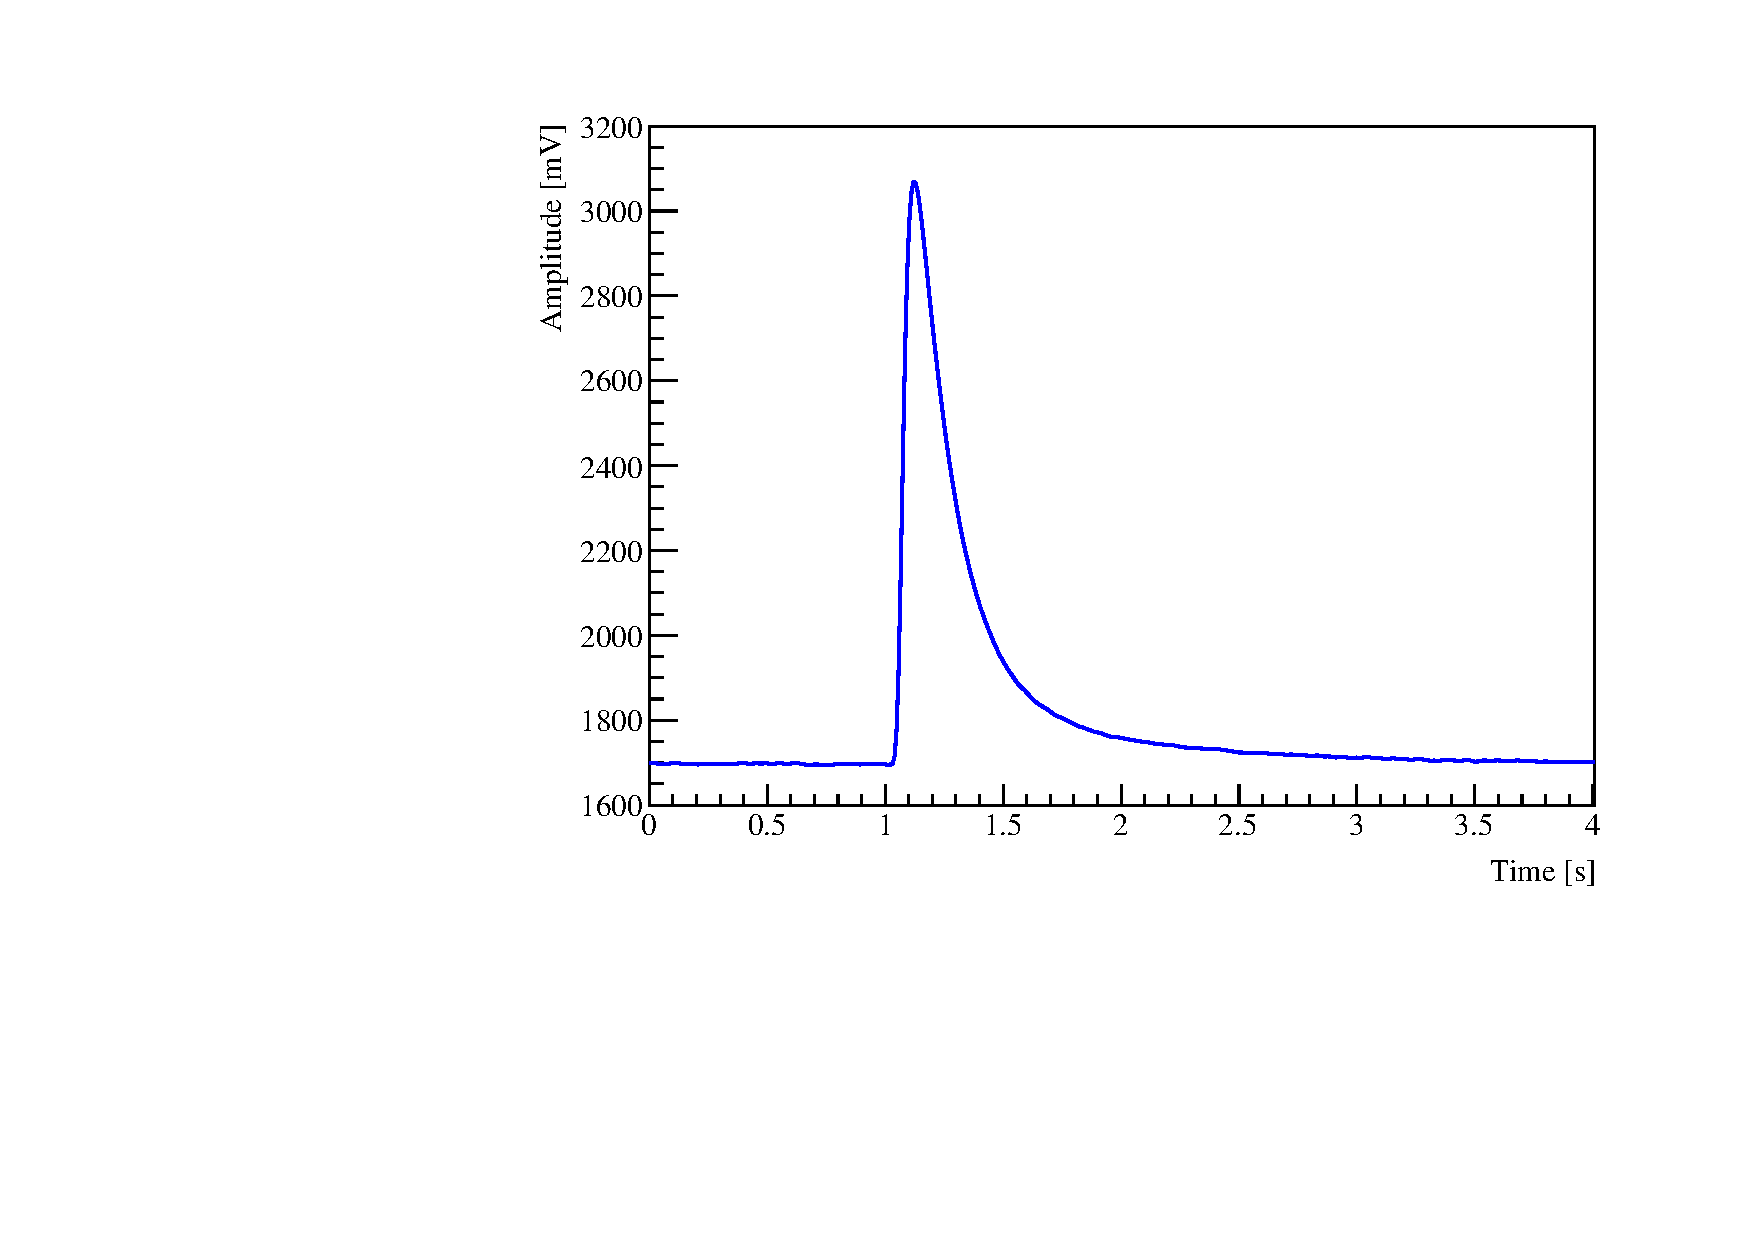
\includegraphics[width=0.7\linewidth]{Figures/pulse-conference.pdf}
\caption[An example pulse from a single CUORE detector measured by an NTD Ge thermistor.]
{An example pulse from a single CUORE detector measured by an NTD Ge thermistor.
After an event at 1 s where energy is deposited in the crystal, a fast (0.1 s) temperature rise is observed followed with a slow (3 s) cooling through the weak coupling to the thermal bath.}
\label{fig:Sample_pulse}
\end{figure}

\subsubsection*{Silicon Heater}
While the detectors are calibrated through physics events on a $\sim$ monthly basis by the calibration system, discussed more in \autoref{chap:DCS}, additional and continuous stabilization is provided through direct heating of the bolometers through a silicon heater that is also attached onto the bolometer, discussed more in \autoref{ssec:Stabilization}.
These heaters are custom-designed $2.33\times2.40\times0.52~\textrm{mm}^3$ high-purity Si chips, shown in \autoref{fig:Si_heater}.
They were manufactured by Istituto per la Ricerca Scientifica e Tecnologica (IRST, now Fondazione Bruno Kessler) in Trento, Italy.
As current passes through these Si chips with resistance $\approx300~\textrm{k}\Omega$, power is dissipated through ohmic losses in the heaters into the bolometers, which is then measured by the NTDs.
By pulsing these heaters with a known energy, the detector response can then be stabilized at various detector baselines.

\begin{figure}
    \centering
    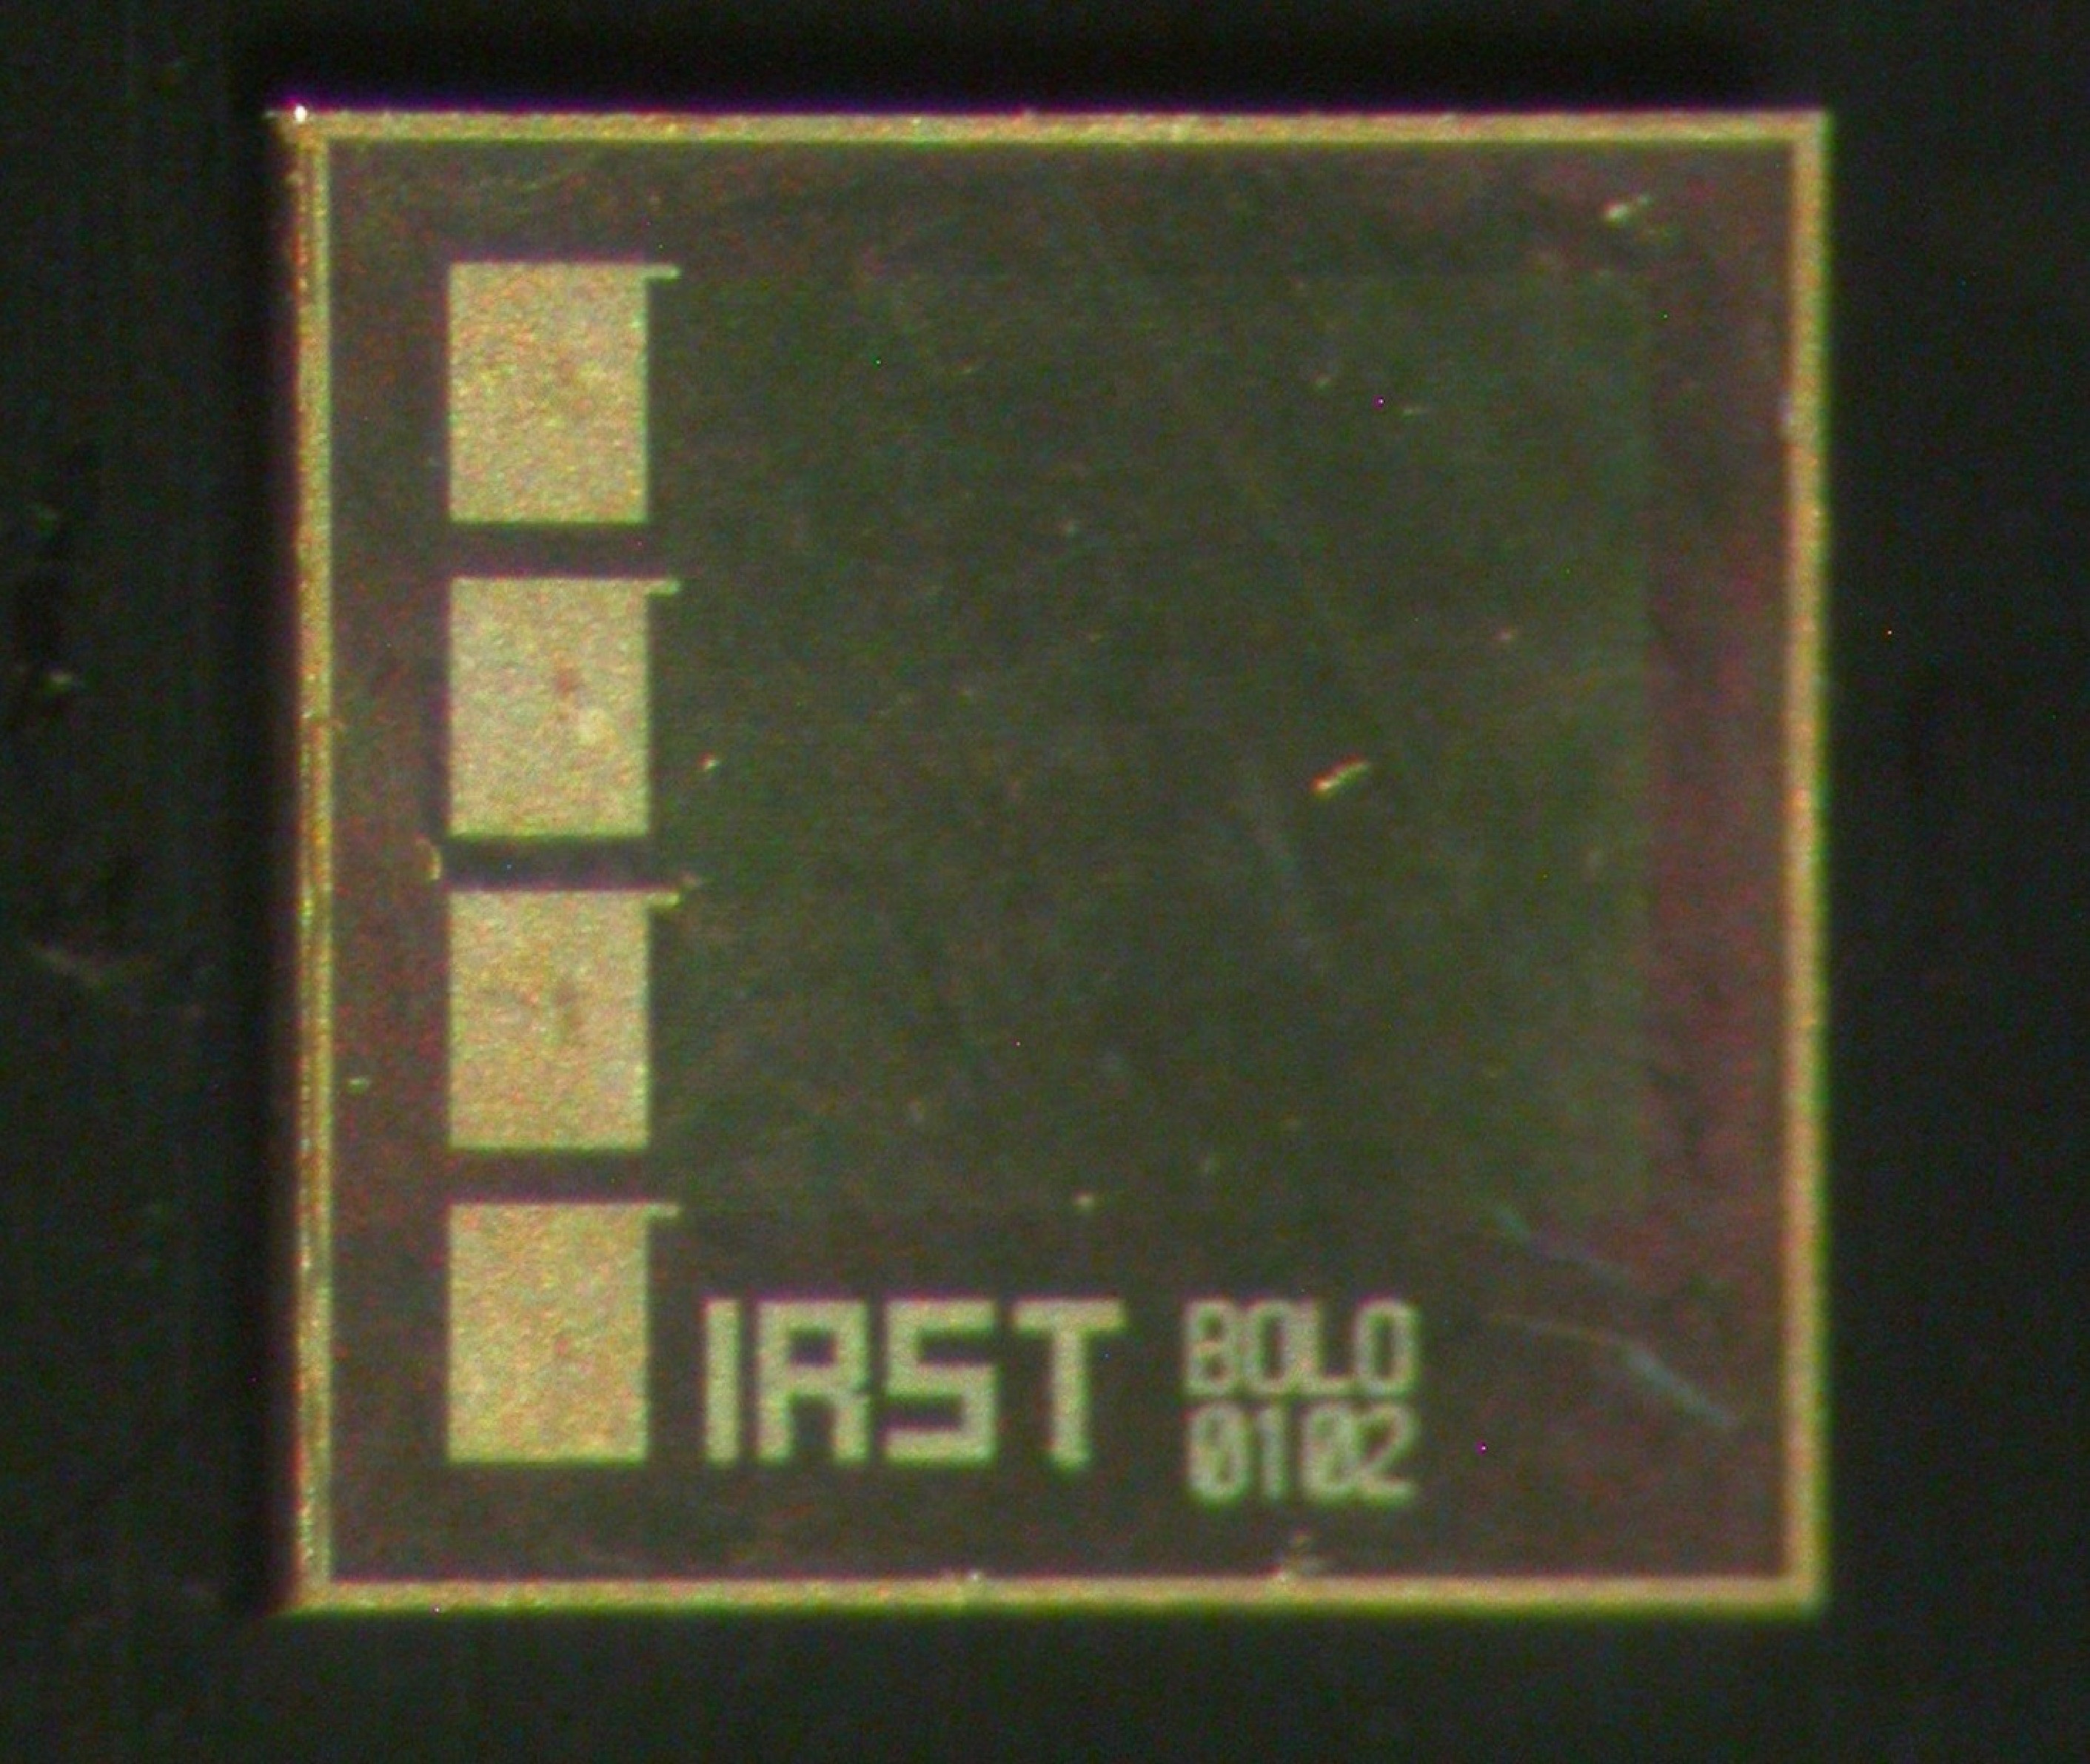
\includegraphics[width=0.4\linewidth]{Figures/fig05a.pdf}
    \caption[Photograph of a silicon heater.]
    {Photograph of a silicon heater.
    There are four aluminum pads on the chip, and, depending on the pair of pads connected, the resistance across the heater can be 100, 200, or 300 k$\Omega$.}
    \label{fig:Si_heater}
\end{figure}

\subsubsection*{Cables and Glue}
The heaters and thermistors need to be attached to the crystals with a strong thermal and mechanical coupling to work properly.
This is done by Araldite Rapid\footnote{\RaggedRight\url{http://www.go-araldite.com/products/epoxy-adhesives/araldite-rapid-2-x-15ml-tube}}
epoxy which is deposited in a pattern of glue spots shown in \autoref{fig:glue}.

\begin{figure}[htbp]
%\captionsetup[subfigure]{justification=centering}
\centering
\begin{subfigure}[t]{0.45\textwidth}
\centering
    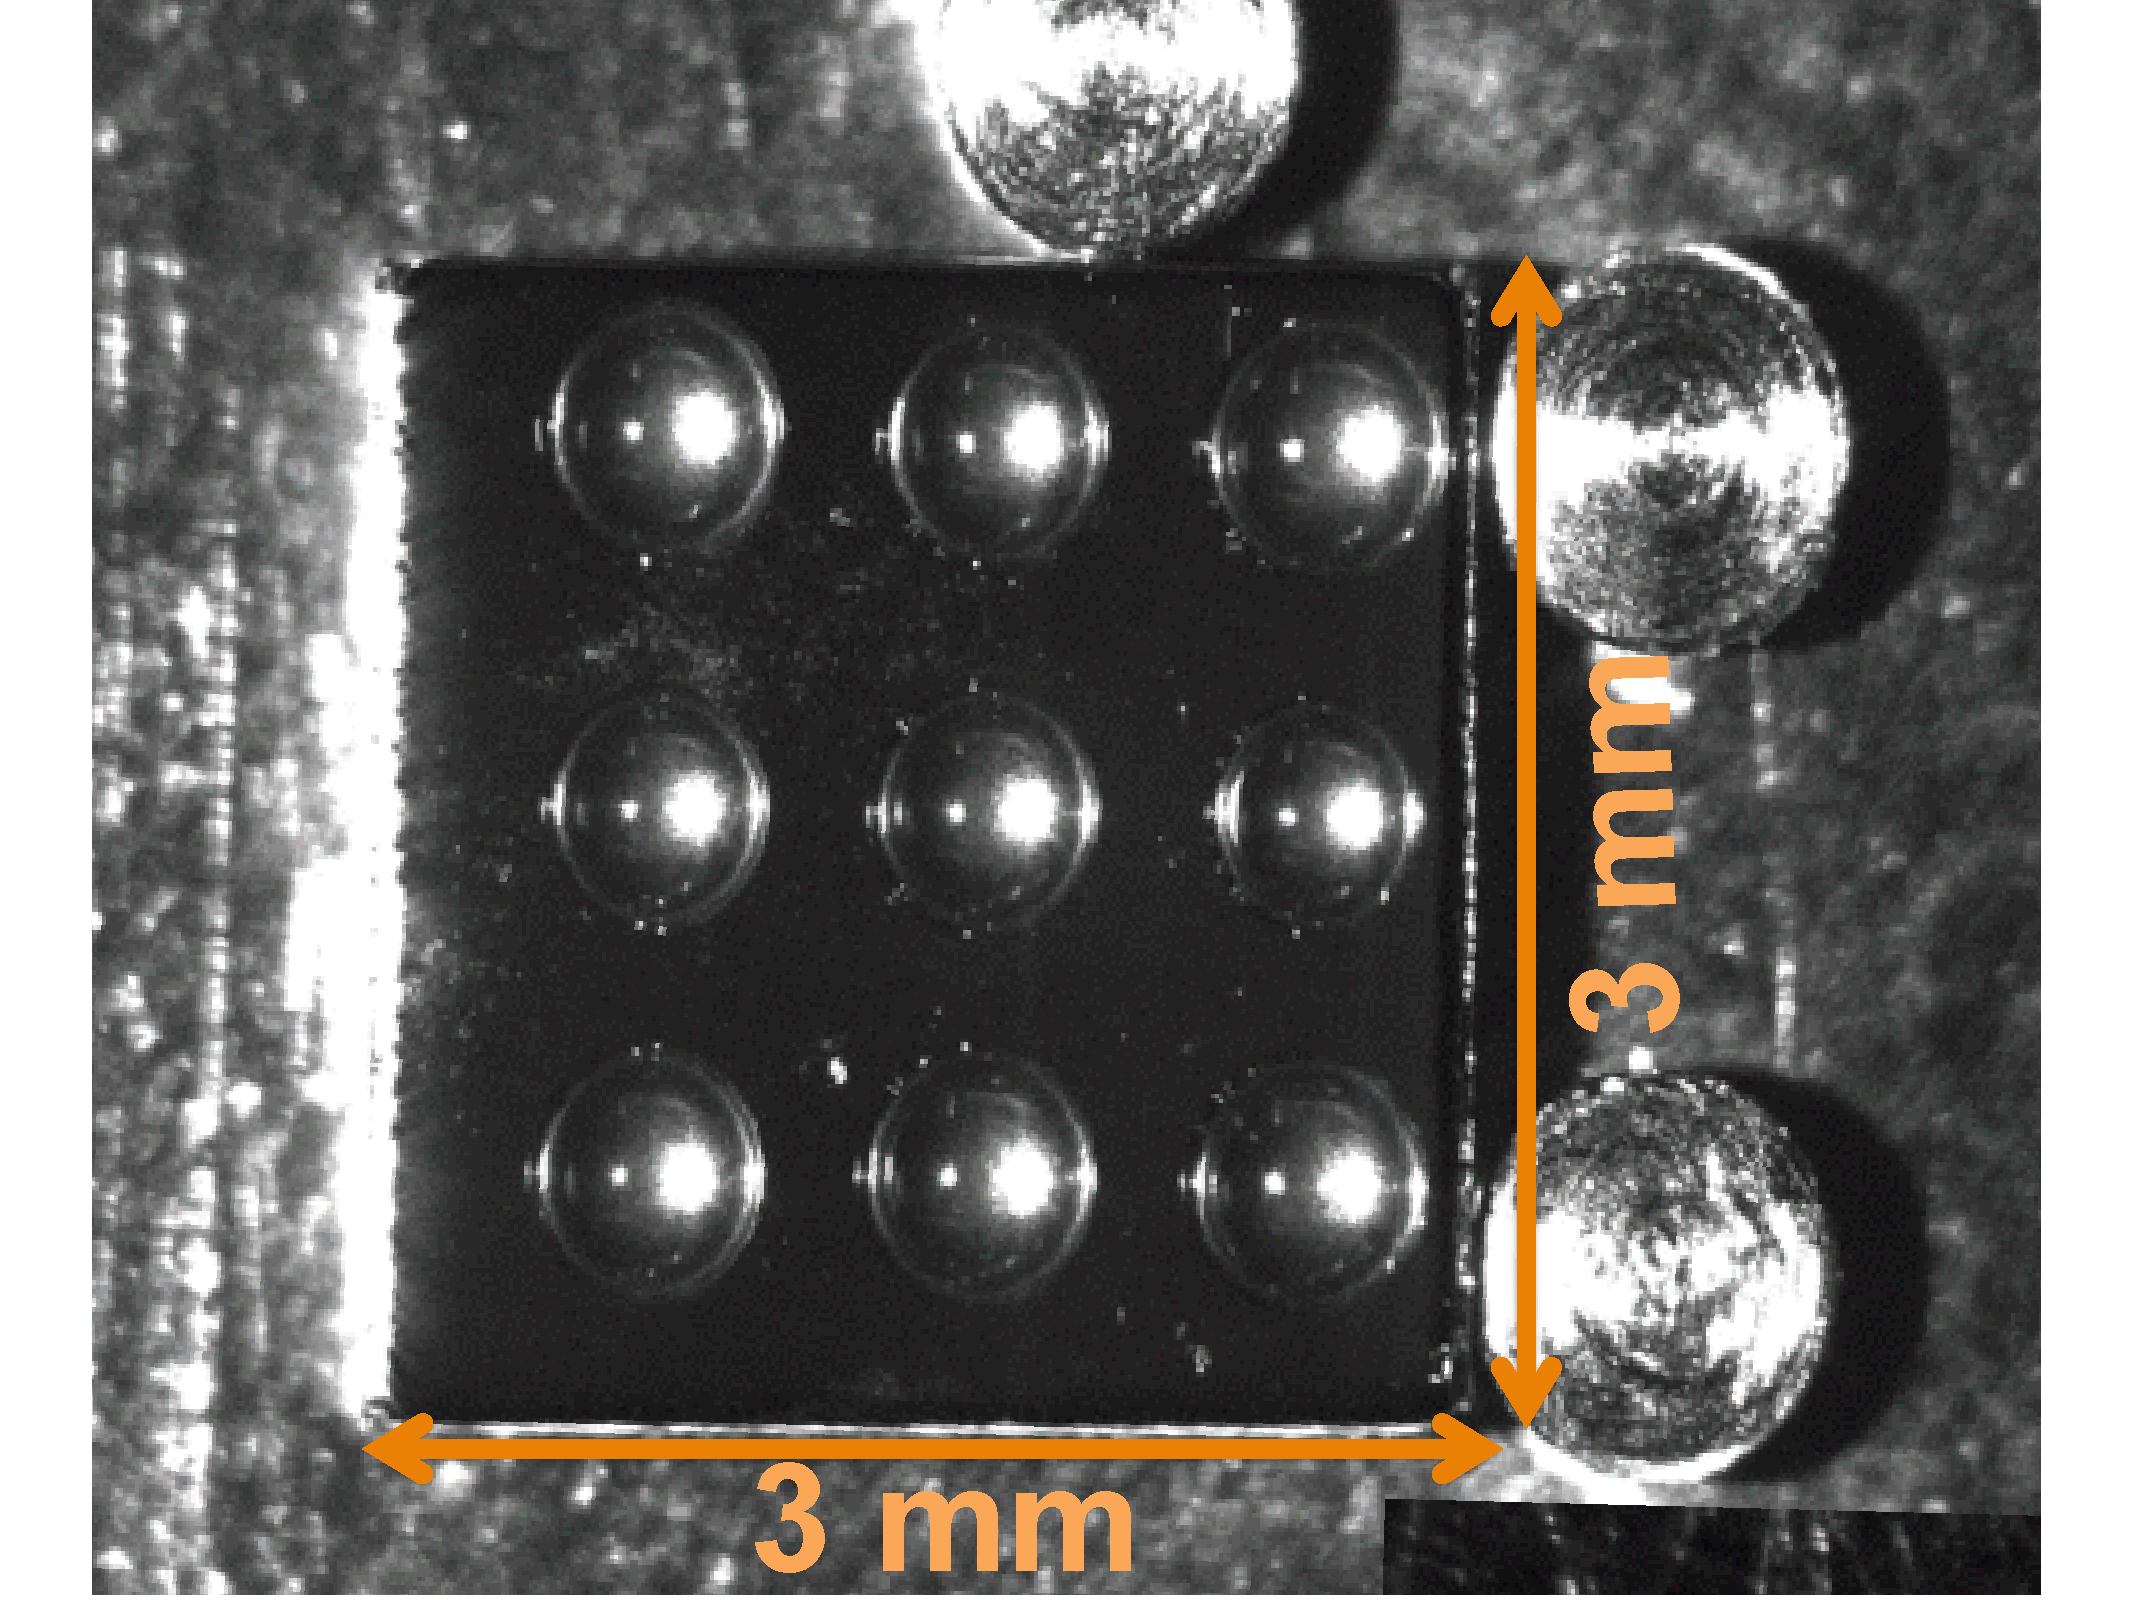
\includegraphics[width=0.95\linewidth]{Figures/fig10a.pdf}
\caption{}
\label{fig:glue_NTD}
\end{subfigure}
\qquad
\begin{subfigure}[t]{0.45\textwidth}
\centering
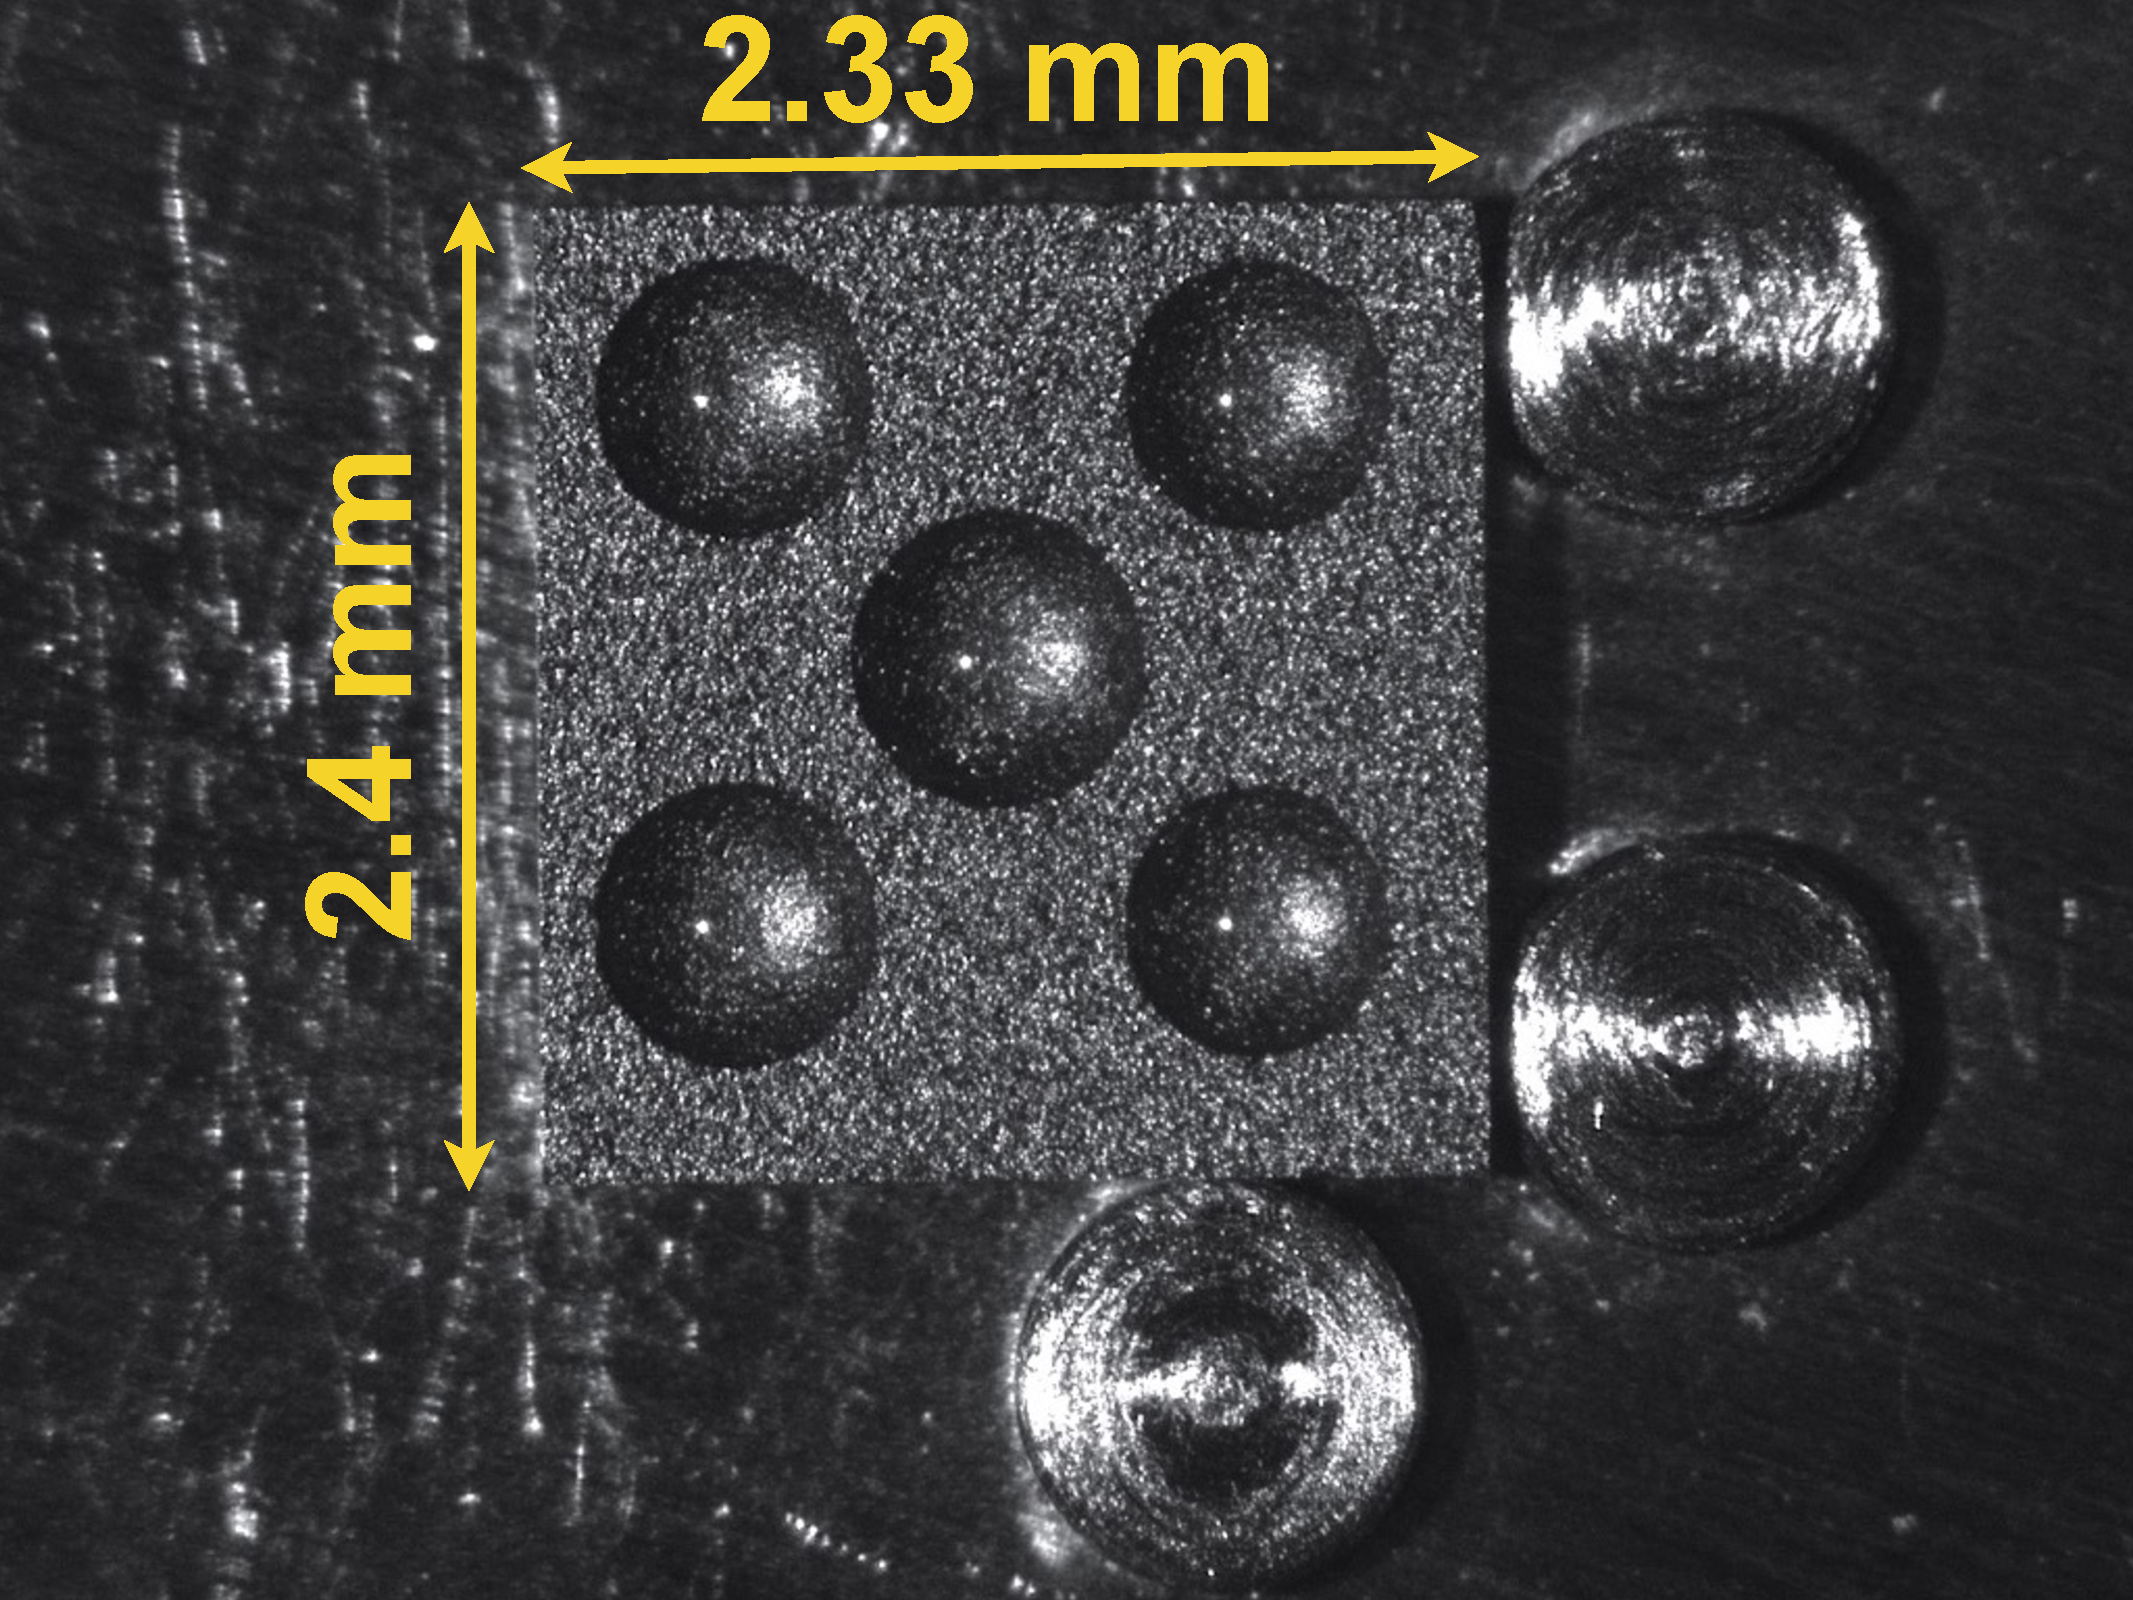
\includegraphics[width=0.95\textwidth]{Figures/fig10b.pdf}
\caption{}
\label{fig:glue_Si}
\end{subfigure}
\caption[Photographs of the glue spots on the CUORE NTD (a) and Si heater (b).]
{Photographs of the glue spots on the CUORE NTD (a) and Si heater (b).
The NTD has a pattern of 9 glue spots and the heater has a pattern of 5 glue spots, applied robotically.
Figure from \cite{Alduino:2016vjd}.}
\label{fig:glue}
\end{figure}

After being glued to each detector, the heater and NTD need to also be connected to the readout electronics.
To achieve this, gold cables are bonded to the pads of the copper tape that is connected to the readout electronics.
Since the NTDs are critically important to the operation of the experiment, these gold cables are doubled for redundancy in case of a poor connection.

\begin{figure}[htbp]
%\captionsetup[subfigure]{justification=centering}
\centering
\begin{subfigure}[t]{0.45\textwidth}
\centering
    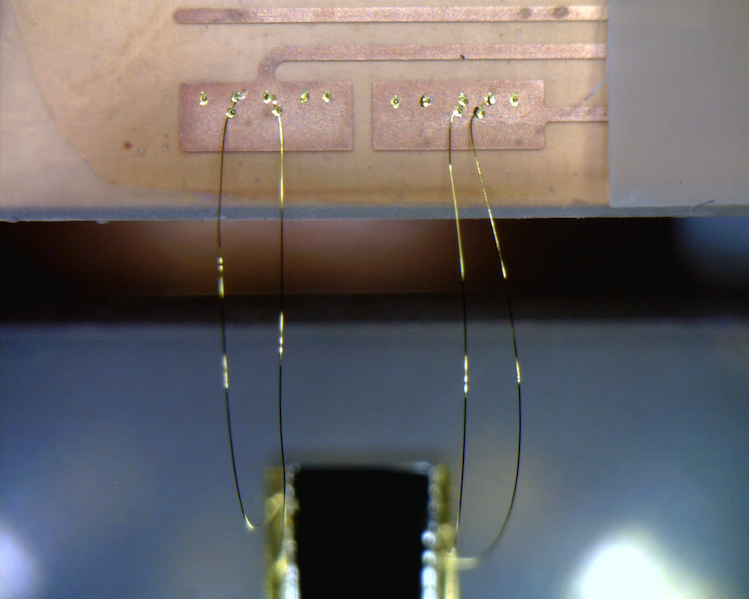
\includegraphics[width=0.95\linewidth]{Figures/NTD_bond.png}
\caption{}
\label{fig:bond_NTD}
\end{subfigure}
\qquad
\begin{subfigure}[t]{0.45\textwidth}
\centering
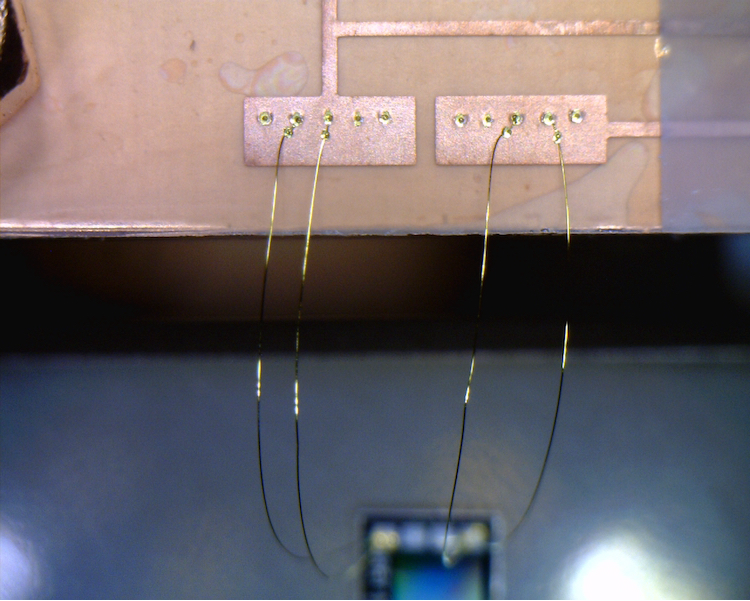
\includegraphics[width=0.95\textwidth]{Figures/Si_bond.png}
\caption{}
\label{fig:bond_Si}
\end{subfigure}
\caption[Photographs of the gold wire bonds on a CUORE NTD (a) and Si heater (b).]
{Photographs of the gold wire bonds on a CUORE NTD (a) and Si heater (b).
Figure courtesy of the CUORE collaboration.}
\label{fig:bonds}
\end{figure}

\subsubsection*{Bolometric Method Drawbacks}
There are some particular challenges to the bolometric method, however.
The dependence on the heat capacity of the crystal depends on the exact crystalline structure of the crystal, which requires regular calibrations due to possible minute changes.
In addition, this strong temperature dependence, while useful for identifying signal, needs a well-stabilized detector with few disturbances from non-particle thermal sources and a consistent and well-understood temperature baseline.
Finally, the long time constant of the cooling of the crystal, which is generally a few seconds for a 1 MeV pulse, requires that there be a low rate of events in the crystal.
This requirement of a low rate is generally not an issue for physics datataking, as the background rates are necessarily low due to the sensitivity requirements of a \zeronubb~search, but this limits the time it takes to calibrate the bolometer\footnote{This generally becomes an optimization problem, later discussed in \autoref{chap:DCS}, where the time it takes to calibrate a detector with 100 events can be reduced by reducing the activity of a calibration source.}.


\subsection{CUORE Detector Array}
CUORE uses 988 \teotwo~crystals as bolometers arranged in 19 towers with 13 floors as shown in \autoref{fig:cuore_detector_array} and \autoref{fig:cuore_photograph}.
These crystals are $5\times5\times5~\textrm{cm}^3$ in size and have mass 750 g each, for a total of 742 kg of \teotwo.
The crystals are grown by The Shanghai Institute of Ceramics, Chinese Academy of Sciences (SICCAS) \cite{Arnaboldi:2010fj} and shipped to Italy by boat, avoiding air travel in order to minimize cosmogenic activation \cite{Barghouty:2010kj}.
Taking advantage of the relatively high natural isotopic abundance of Te, shown in \autoref{fig:q_vs_ia-color}, this comes to a total mass of 206 kg of $^{130}$Te and 189 kg of $^{128}$Te.
Each tower is approximately 80 cm tall, such that in operation, these crystals form the coldest cubic meter in the known universe \cite{Ouellet:2014qua}.

\begin{figure}
    \centering
    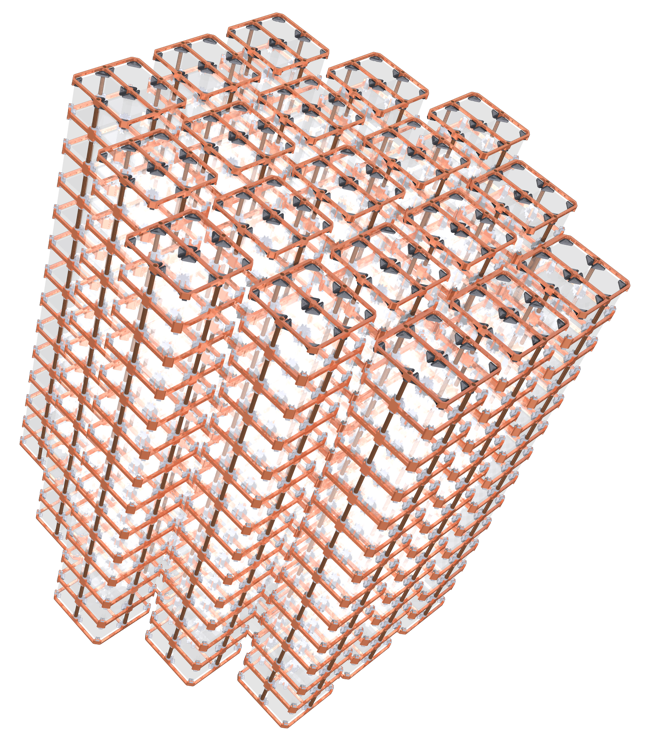
\includegraphics[height=4in]{Figures/CUORE_detector_array_0.png}
    \caption[A schematic of the CUORE detector array.]
    {A schematic of the CUORE detector array.
    The detectors are held in place by the copper frames and arranged in 19 towers with 13 floors each.
    The position of the detector array relative to the rest of the cryostat can be seen in \autoref{fig:cryostat_cad_cutout}.}
    \label{fig:cuore_detector_array}
\end{figure}

Another benefit to using a bolometric method for particle detection is that it enables a ``source $=$ detector" style experiment such that the \zeronubb~and \twonubb~decays happen directly inside the detectors themselves.
This both reduces the amount of material and associated radioactive backgrounds needed in the experiment and also increases the signal detection efficiency of \zeronubb~and \twonubb-like decays.

In order to arrange these bolometers into these 19 towers, the \teotwo~crystals are held together inside copper frames with polytetrafluoroethylene (PTFE) holders.
These holders are designed such that the crystals are held in place firmly at the low temperatures in CUORE\footnote{Although, one of the benefits of using \teotwo~is that its thermal contraction is similar to that of copper, with values of $\Delta l/l \approx 0.27\%$ and $\Delta l / l \approx 0.33\%$, respectively \cite{ALESSANDRELLO1995363}.}.
A rendering of a CUORE tower is shown in \autoref{fig:tower_rendering}.

\begin{figure}
    \centering
    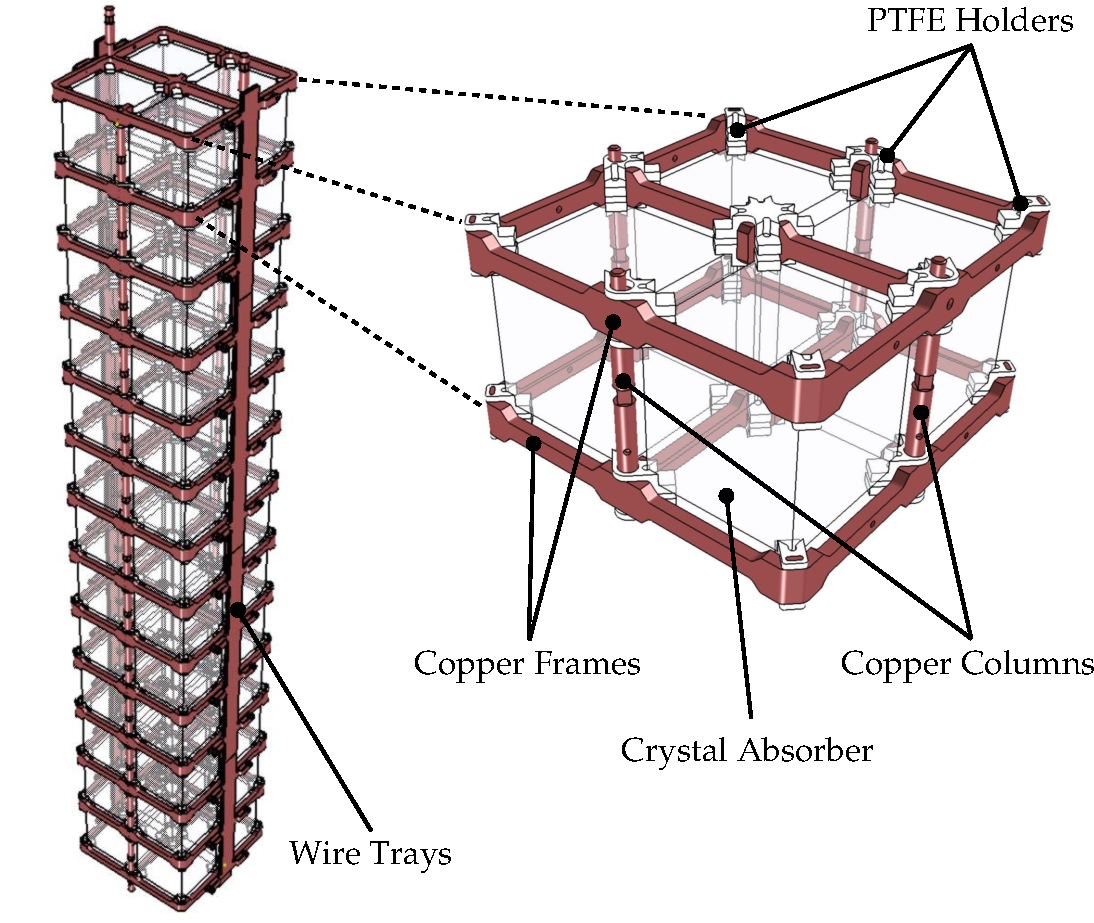
\includegraphics[width=0.8\linewidth]{Figures/fig02.pdf}
    \caption[A rendering of the components of a single CUORE tower (left) and floor (right).]
    {A rendering of the components of a CUORE tower (left) and floor (right).
    The copper frames are shared between floors, and only the PTFE and the gold wiring connecting the silicon heaters and NTD thermistors to the wiring on the frames act as the weak thermal contact to the detectors.
    Figure from \cite{Alduino:2016vjd}.}
    \label{fig:tower_rendering}
\end{figure}
It is important to note that the number and size of each component on the towers is minimized as much as possible, while keeping the structural integrity intact.
Since these components are the nearest to the detectors, keeping their radioactivity to a minimum significantly lowers the background and is discussed more in \autoref{ssec:CUORE-0}.
This was one of the improvements from Cuoricino's towers to CUORE's towers, as the amount of copper used in the frames was able to be reduced by a factor of $\sim2.5$.

As shown in \autoref{fig:tower_rendering}, there are trays on opposite sides of the tower.
These wire trays contain copper-insulator tape with a polyethylene naphthalate substrate (referred to as ``Cu-PEN" tape) and are used to electrically connect the NTD thermistors and the Si heaters on the detectors to the other NbTi cabbles that connect to the electronics at the top of the cryostat.
These cables have a length of 1.4 meters with a thickness of 80 $\mu \textrm{m}$ and a pattern of traces in the 17 $\mu \textrm{m}$ thick copper layer.
As the detectors are read out through these connections, they must have low cross-talk and microphonic pickup in addition to their background requirements.
Two sets of these cables are connected to two opposing sides of the towers, and branch out to connect to crystals on each floor.
These tapes  are divided into 4 types, depending on how far down along the tower they reach, and a separate tape is used for the Si heaters.
A photograph of these tapes is shown in \autoref{fig:CuPEN}.

\begin{figure}
    \centering
    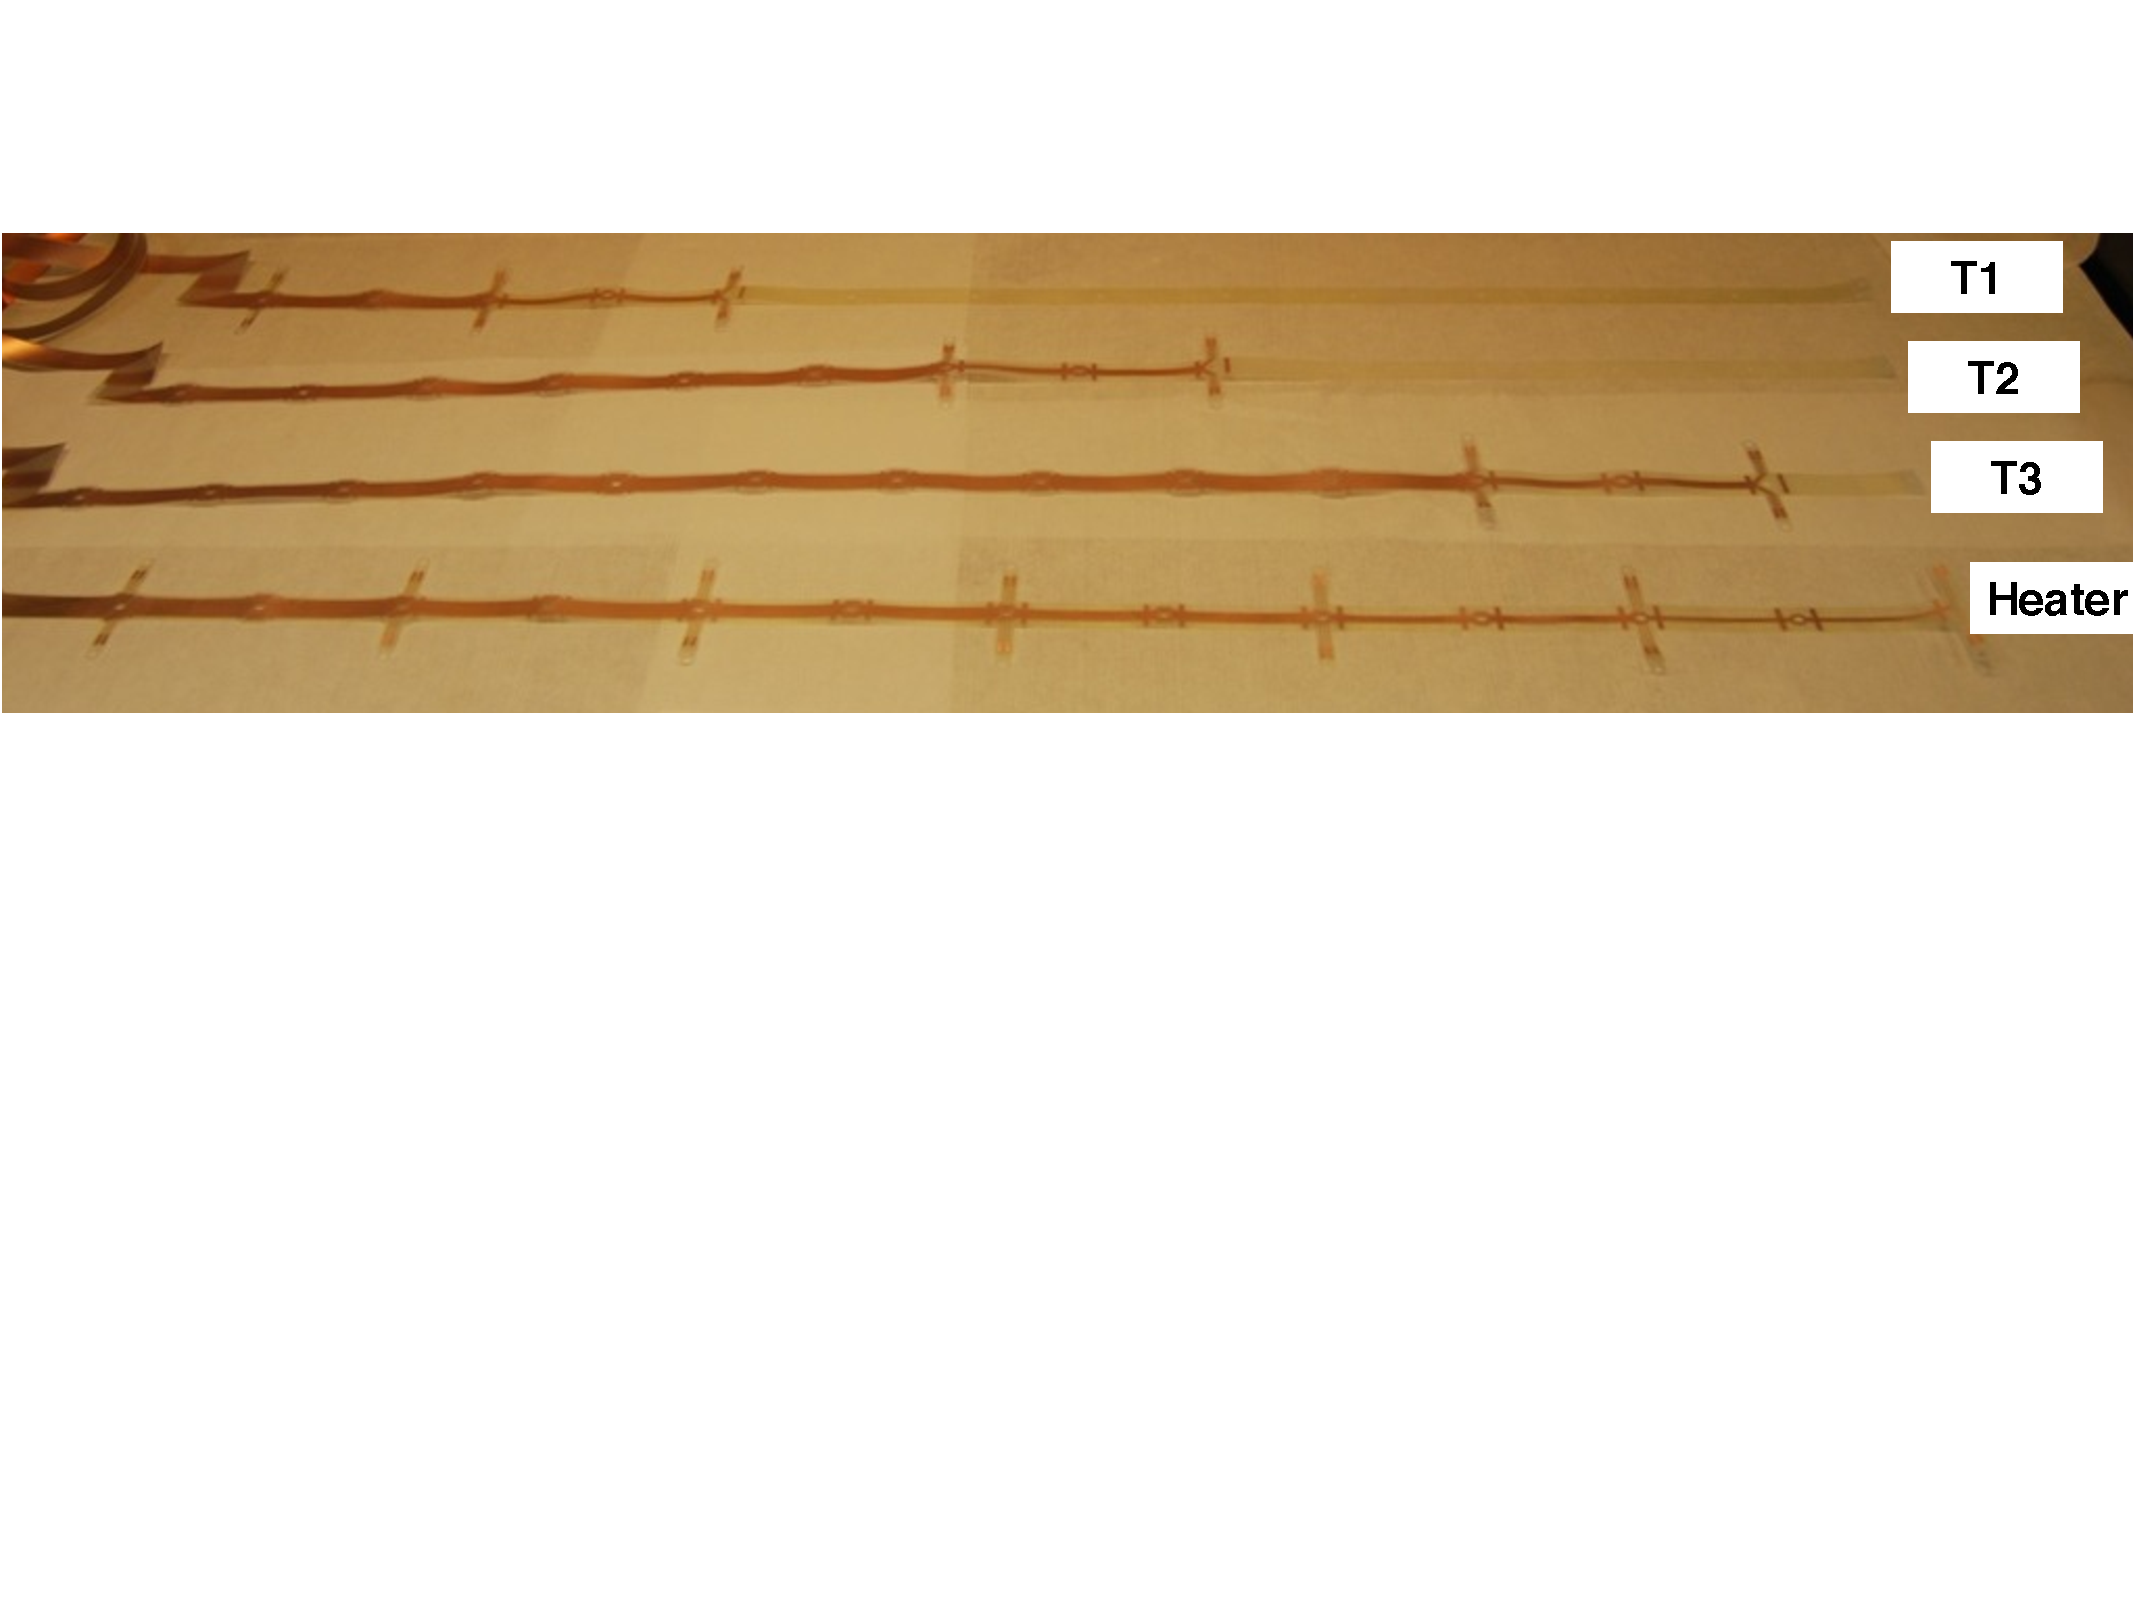
\includegraphics[width=0.9\linewidth]{Figures/fig07.pdf}
    \caption[A photograph of the Cu-PEN tapes that are placed inside the wire trays on the CUORE towers.]
    {A photograph of the Cu-PEN tapes that are placed inside the wire trays on the CUORE towers.
    The numbered tapes connect to floors 9-13, 5-8, and 1-4, respectively counting from the bottom of the tower, and the Heater tape contains two sets of signals to connect to a single column each.
    Figure from \cite{Alduino:2016vtd}.}
    \label{fig:CuPEN}
\end{figure}

\subsection{CUORE Tower Construction and Assembly}

\subsubsection{Crystal Growth}
As mentioned in the preceeding section, the first part of the detector construction and tower assembly occurrs with growth of the Te crystals at SICCAS.
This growth was performed in two phases: crystal growth and crystal polishing.
During each procedure, extreme care was taken to minimize bulk contaminations forming in the first phase and surface contaminations in the second \cite{crystal_growth_methods, crystal_growth_methods_2, Barghouty:2010kj}.
During the first procedure, the crystals are grown twice, where, after the first growth, 1 mm is removed from the ingots and the selected best sections of the first growth are used as high-purity powder for the second.
This two-stage growth process enables crystal purity of 99.999\%, up from the 99.99\% purity of commercially available powder.
This increased purity, along with growing the crystals from powder, strongly reduces bulk contaminations of $^{40}$K, which is a particularly problematic background for \twonubb~measurements, as it decays through beta-decay.

After the crystals are grown, they are then cut into cubes with $5 \pm 0.0050$ cm edges and $0.05$ cm chamfers with an average flatness on each face of $<0.001$ cm.
In addition, the cubic faces are oriented parallel to the planes of the crystalline structure of the \teotwo~within $\pm1^{\circ}$ by means of an X-ray on the crystals after their growth.
The cleaning process then takes two steps: first, by means of chemical etching, and, second, by polishing the crystals.
Each of these processes removes approximately $10^5$ atomic layers from the surface of the crystal, which removes surface impurities that may have adsorbed onto the crystal surface and begun to diffuse into the bulk.
At the end of the polishing step, the completed crystal is then triple-bagged in vacuum and stored in groups of 6 in a polyethylene vacuum box in order to avoid exposure to atmospheric radon.

Once the crystals arrive at LNGS, they are immediately placed in storage underground under a flux of nitrogen.
Despite the short $\sim$1 month that the crystals are aboveground causes the crystals to have cosmogenic activation of $^{110m}$Ag and $^{60}$Co that contribute $<1\%$ of the background at the Q-value of $^{130}$Te \cite{PhysRevC.92.024620, BARGHOUTY201316}.

\subsubsection{Parts Selection and Cleaning}
\label{ssec:Parts Selection and Cleaning}
The copper used to house the detectors in the detector array also undergoes an extensive cleaning process.
The copper selected for this is produced by Arubis\footnote{Originally named Norddeutsche Affinerie.} and is their high-purity Electrolytic Tough Pitch (ETP1) copper alloy, called NOSV\footnote{\RaggedRight\url{http://www.aurubis.com/en/our-business/products/aurubis-shapes/materials/shapes-materials-table}}.
This copper was chosen for CUORE due to its radiopurity and its high residual resistance ratio, certified to be over 400.
However, while the bulk contamination of NOSV copper is low, the surface contaminations of commercially-available NOSV copper due to its handling and machining.
This required the development of a stringent cleaning procedure that involved a sequence of tumbling and chemical etching.
In addition, the larger copper shields facing the detector were wrapped in polyethlyene film while the small copper parts on the towers were also subjected to Magnetron plasma etching, TECM.
This cleaning procedure required the copper to be above ground for a total of 4 months between casting and storage underground.
During this time, the cosmogenic activity for CUORE data-taking is estimated to be a negligible value of <50 $\mu$Bq$/$kg.
These procedures were validated during the Three Towers Test  and the surface contamination of the cleaned NOSV copper was measured to be 3.8 nBq/cm$^2$ and 2.0 nBq/cm$^2$ for $^{238}$U and $^{232}$Th, respectively \cite{ALESSANDRIA201313}.
The other components on the CUORE towers, viz. the NTDs, the silicon heaters, PTFE holders, etc., are also subjected to a cleaning process and are stored under a nitrogen flux before assembly.
The final bulk and surface contaminations of the components of the CUORE tower are shown in \autoref{tab:NearDetectorSources_Bulk} and \autoref{tab:NearDetectorSources_Surface}, respectively.

\begin{table}[htbp]
\centering
\caption[90\% C.L. upper limits of $^{232}$Th and $^{238}$U bulk contamination of sources near the detector.]
{90\% upper limits of $^{232}$Th and $^{238}$U bulk contamination of sources near the detector.
Table from \cite{Alduino:2017qet}.}
\label{tab:NearDetectorSources_Bulk}
\begin{tabular}{lll}
\hline
\hline
Material         & $^{232}$Th [Bq/kg]         & $^{238}$U [Bq/kg]    \\
\hline
TeO2             & $<8.4\times10^{-7}$ & $<6.7\times10^{-7}$      \\
Glue             & $<8.9\times10^{-4}$ & $<1.0\times10^{-2}$          \\
Au bonding wires & $<4.1\times10^{-2}$ & $<1.2\times10^{-2}$       \\
Si heaters       & $<3.3\times10^{-4}$ & $<2.1\times10^{-3}$        \\
NTDs             & $<4.1\times10^{-3}$ & $<1.2\times10^{-2}$    \\
Cu-PEN           & $<1.0\times10^{-3}$ & $<1.3\times10^{-3}$ \\
PTFE             & $<6.1\times10^{-6}$ & $<2.2\times10^{-5}$       \\
Cu NOSV           & $<2.1\times10^{-6}$ & $<6.5\times10^{-5}$    \\
\hline
\hline
\end{tabular}
\end{table}

\begin{table}[htbp]
\centering
\caption[90\% C.L. upper limits of $^{232}$Th, $^{238}$U, and $^{210}$Pb surface contamination and the contamination depth of sources near the detector.]
{90\% C.L. upper limits of $^{232}$Th, $^{238}$U, and $^{210}$Pb surface contamination and the contamination depth of sources near the detector.
Table from \cite{Alduino:2017qet}.}
\label{tab:NearDetectorSources_Surface}
\begin{tabular}{lllll}
\hline
\hline
Material         & Depth [$\mu$m] & $^{232}$Th [Bq/kg]         & $^{238}$U [Bq/kg]     & $^{210}$Pb [Bq/cm$^2$] \\
\hline
TeO2  & 0.01-10 & $<1.9\times10^{-9}$ & $<8.9\times10^{-9}$ & $<9.8\times10^{-7}$ \\
Si heaters  & 0.1-10 & $<3.3\times10^{-6}$ & $<8.2\times10^{-7}$ & $<8.2\times10^{-7}$ \\
NTDs  & 0.1-10 & $<8.0\times10^{-6}$ & $<5.0\times10^{-6}$ & $<4.0\times10^{-5}$ \\
Cu-PEN  & 0.1-30 & $<4.0\times10^{-6}$ & $<5.0\times10^{-6}$ & $<3.0\times10^{-5}$ \\
PTFE  & 0.1-30 & $<1.9\times10^{-8}$ & $<6.8\times10^{-8}$ & - \\
Cu NOSV & 0.1-10 & $<6.8\times10^{-8}$ & $<6.5\times10^{-8}$ & $<8.6\times10^{-7}$ \\
\hline
\hline
\end{tabular}
\end{table}

\subsubsection{Tower Assembly}
\label{ssec:Tower Assembly}
Assembling the towers components takes place in two stages.
First, a semi-automated workstation was set up to glue the NTD and Si heater chips to the crystals, and then another workstation with task-specific glove boxes for the assembly.
The activities were undertaken in a class 1000 (ISO 6) cleanroom in the same underground hut at LNGS as the CUORE cryostat.
During the entire assembly process, the tower materials are held in a nitrogen-flushed environment and contact with other materials is minimized to prevent contaminations.

For gluing the NTDs and Si heaters to the crystals, a six-axis articulated robotic arm lifts and positions the crystals, which are then glued by a three-axis Cartesian robot.
The glue dots are applied in the dot pattern shown in \autoref{fig:glue} as there is a mismatch between the thermal expansion coefficients for the components.
This pattern balances the need for good thermal coupling with the mechanical stress resulting from cooling down the crystals.
The use of a semi-automated system was learned from the experience in the Cuoricino experiment, where manual gluing strongly affected the signal shapes\footnote{Not to mention scaling up to 988 crystals in CUORE requires more uniformity and less manually-intensive labor per crystal/tower.}.
The setup used for the entire gluing process is shown in \autoref{fig:gluing_workstation}.

\begin{figure}[htbp]
    \centering
    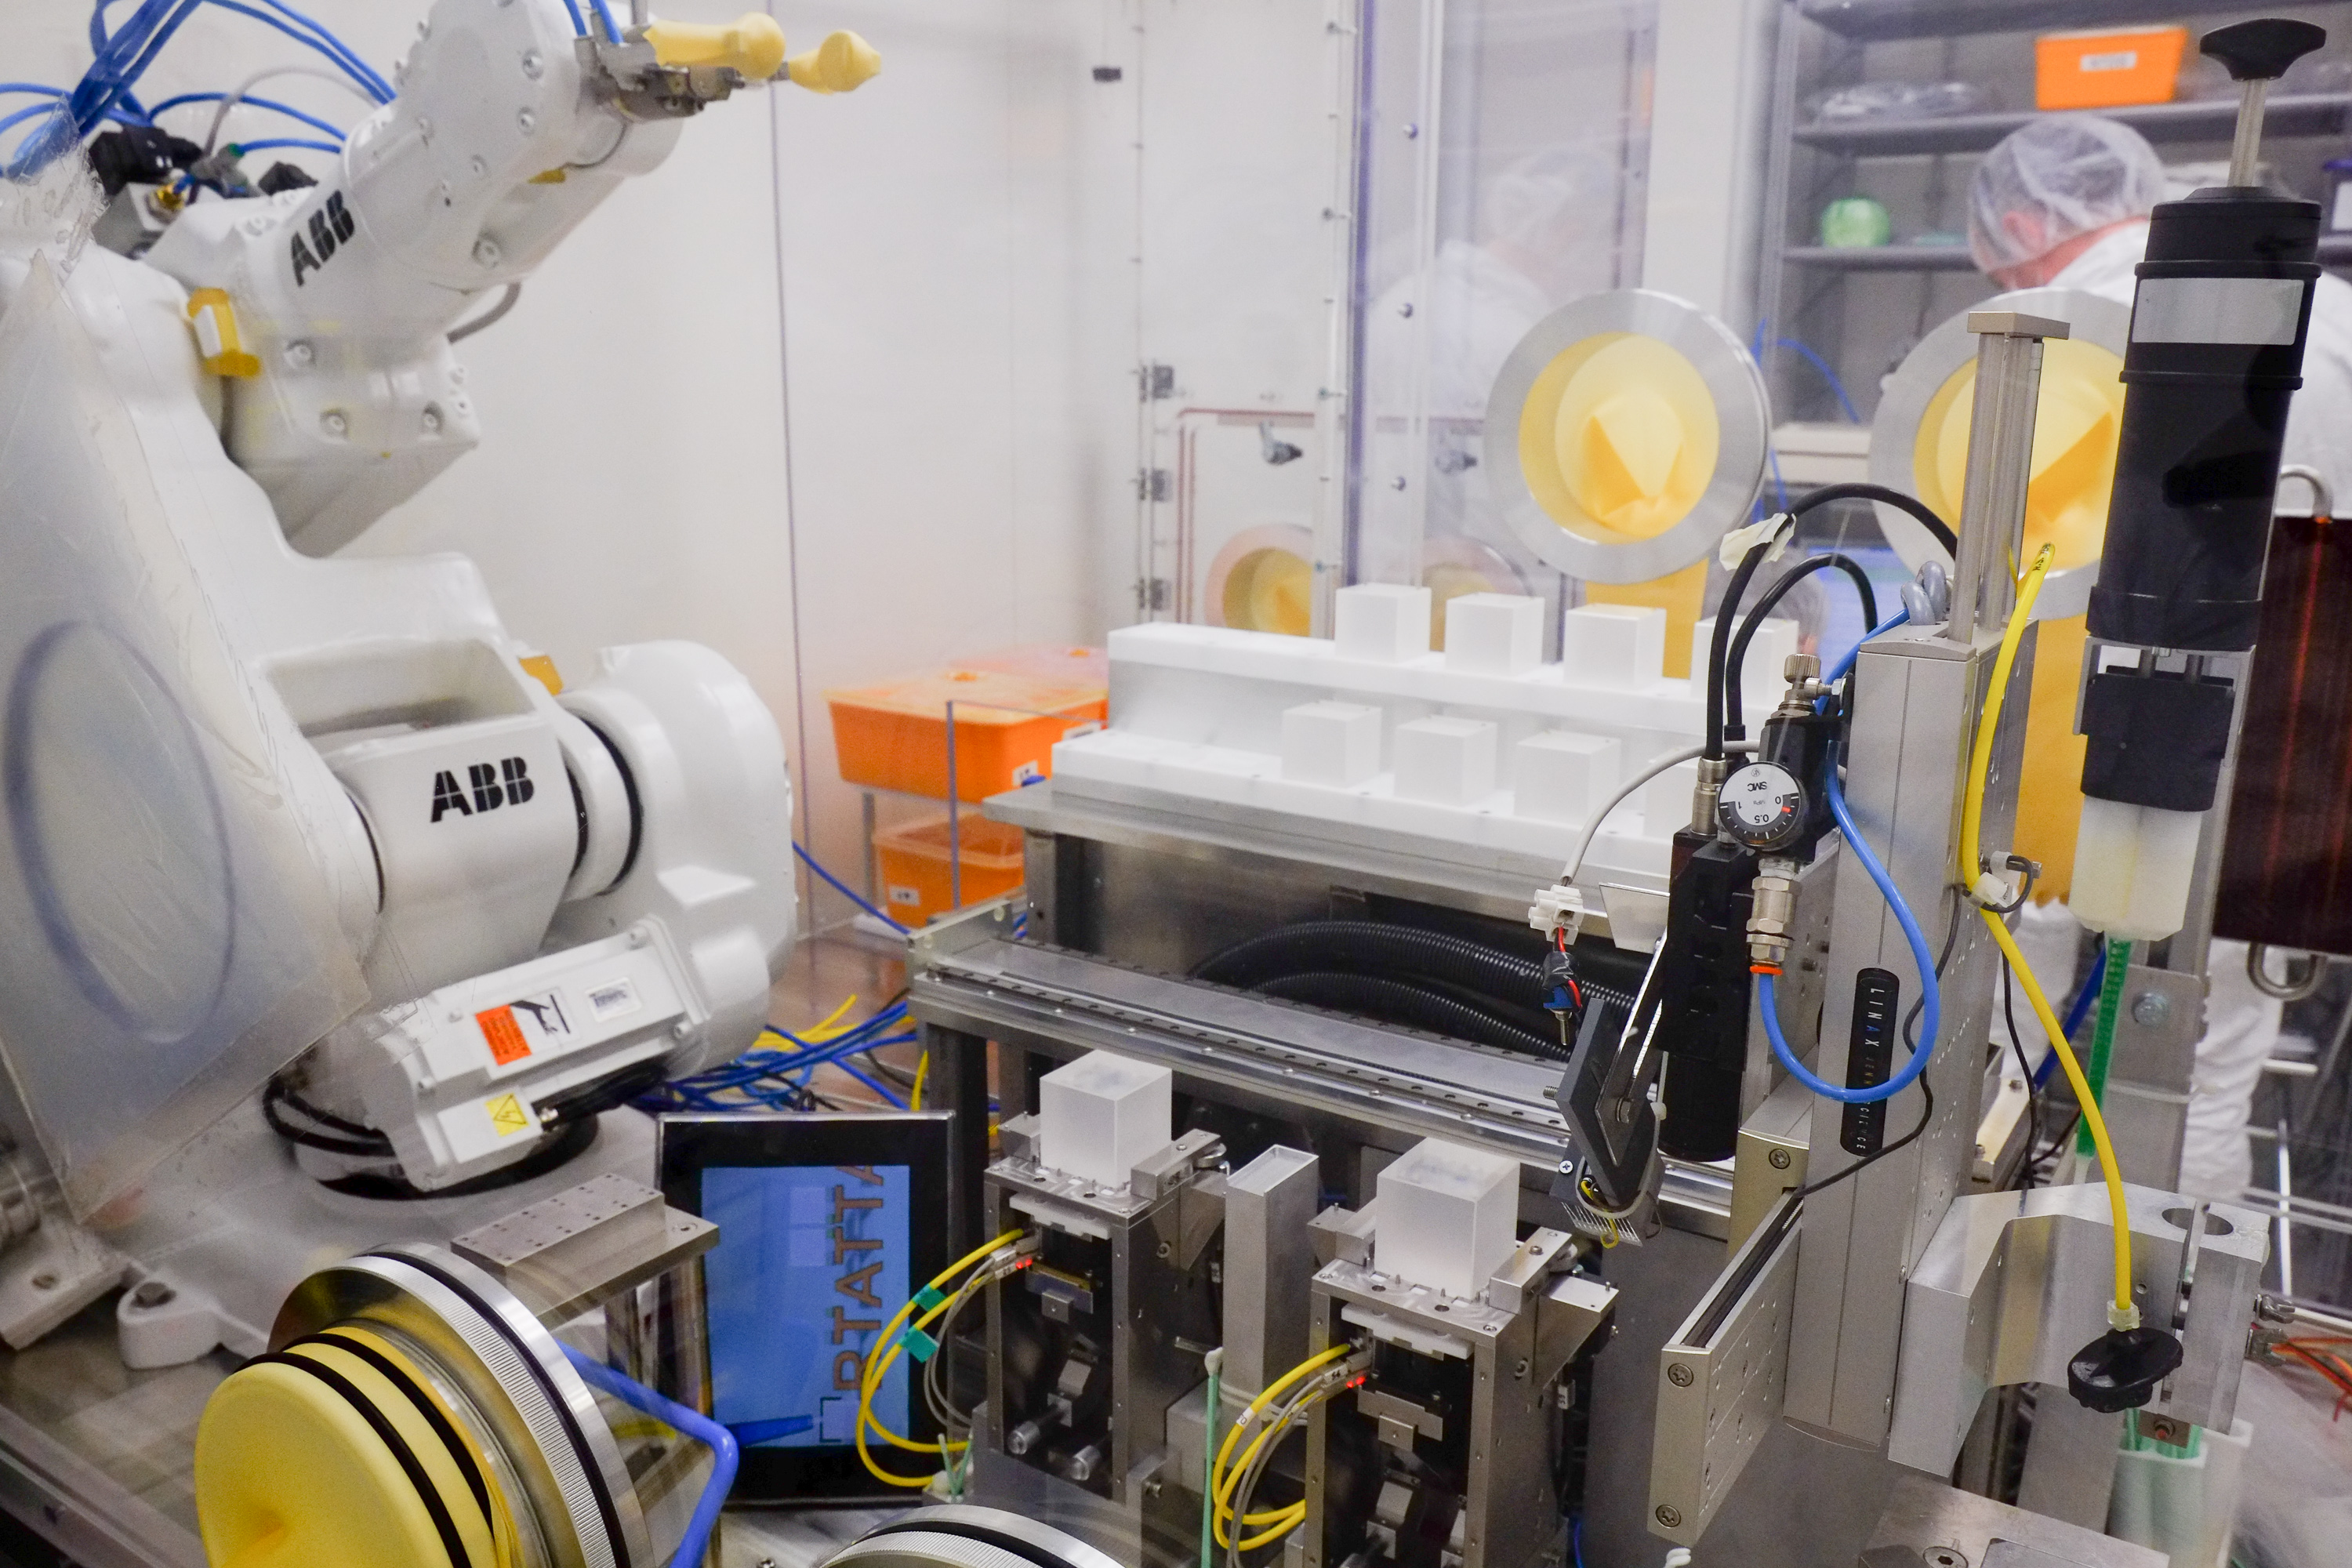
\includegraphics[width=0.7\linewidth]{Figures/cuore_gluing_pic1.jpg}
    \caption[The CUORE gluing workstation.]
    {The CUORE gluing workstation.
    On the left, the robotic arm lifts and moves the crystals, which can be seen on the workstation in the center, as needed for the gluing process.
    The Cartesian robot is on the right side of the workstation, along with the glue mixer.
    Photograph courtesy of the CUORE collaboration.}
    \label{fig:gluing_workstation}
\end{figure}

In the gluing process, the NTD thermistor and Si heater are placed upside down and then the mixed epoxy is injected into a syringe on the Cartesian robot and deposited onto the chips.
After the dots are inspected, a crystal is then taken from the shelf and placed above the chips with a hard face of the crystal facing the chips.
During this time, vacuum suction is used to keep the crystals at a distance of 50$\pm 5~\mu$m from the chips.
This whole process takes three minutes, taking into account the setting time of the epoxy.
After the crystal is glued, allowing as a precaution an hour for the epoxy to cure, the glued crystals are then removed from the glove box inside a vacuum-sealed box and placed into nitrogen-flushed storage.

After the gluing is completed, the assembly of the tower begins.
This is done at a separate workstation which consists of a ``garage" flushed with nitrogen to store the tower and a specialized glovebox that can couple to the garage depending on the task at hand.
First, the assembly takes place one floor at a time, with the crystals being placed in the teflon supports in the NOSV coper structure.
This assembly is shown in \autoref{fig:assemblybox}.

\begin{figure}[htbp]
    \centering
    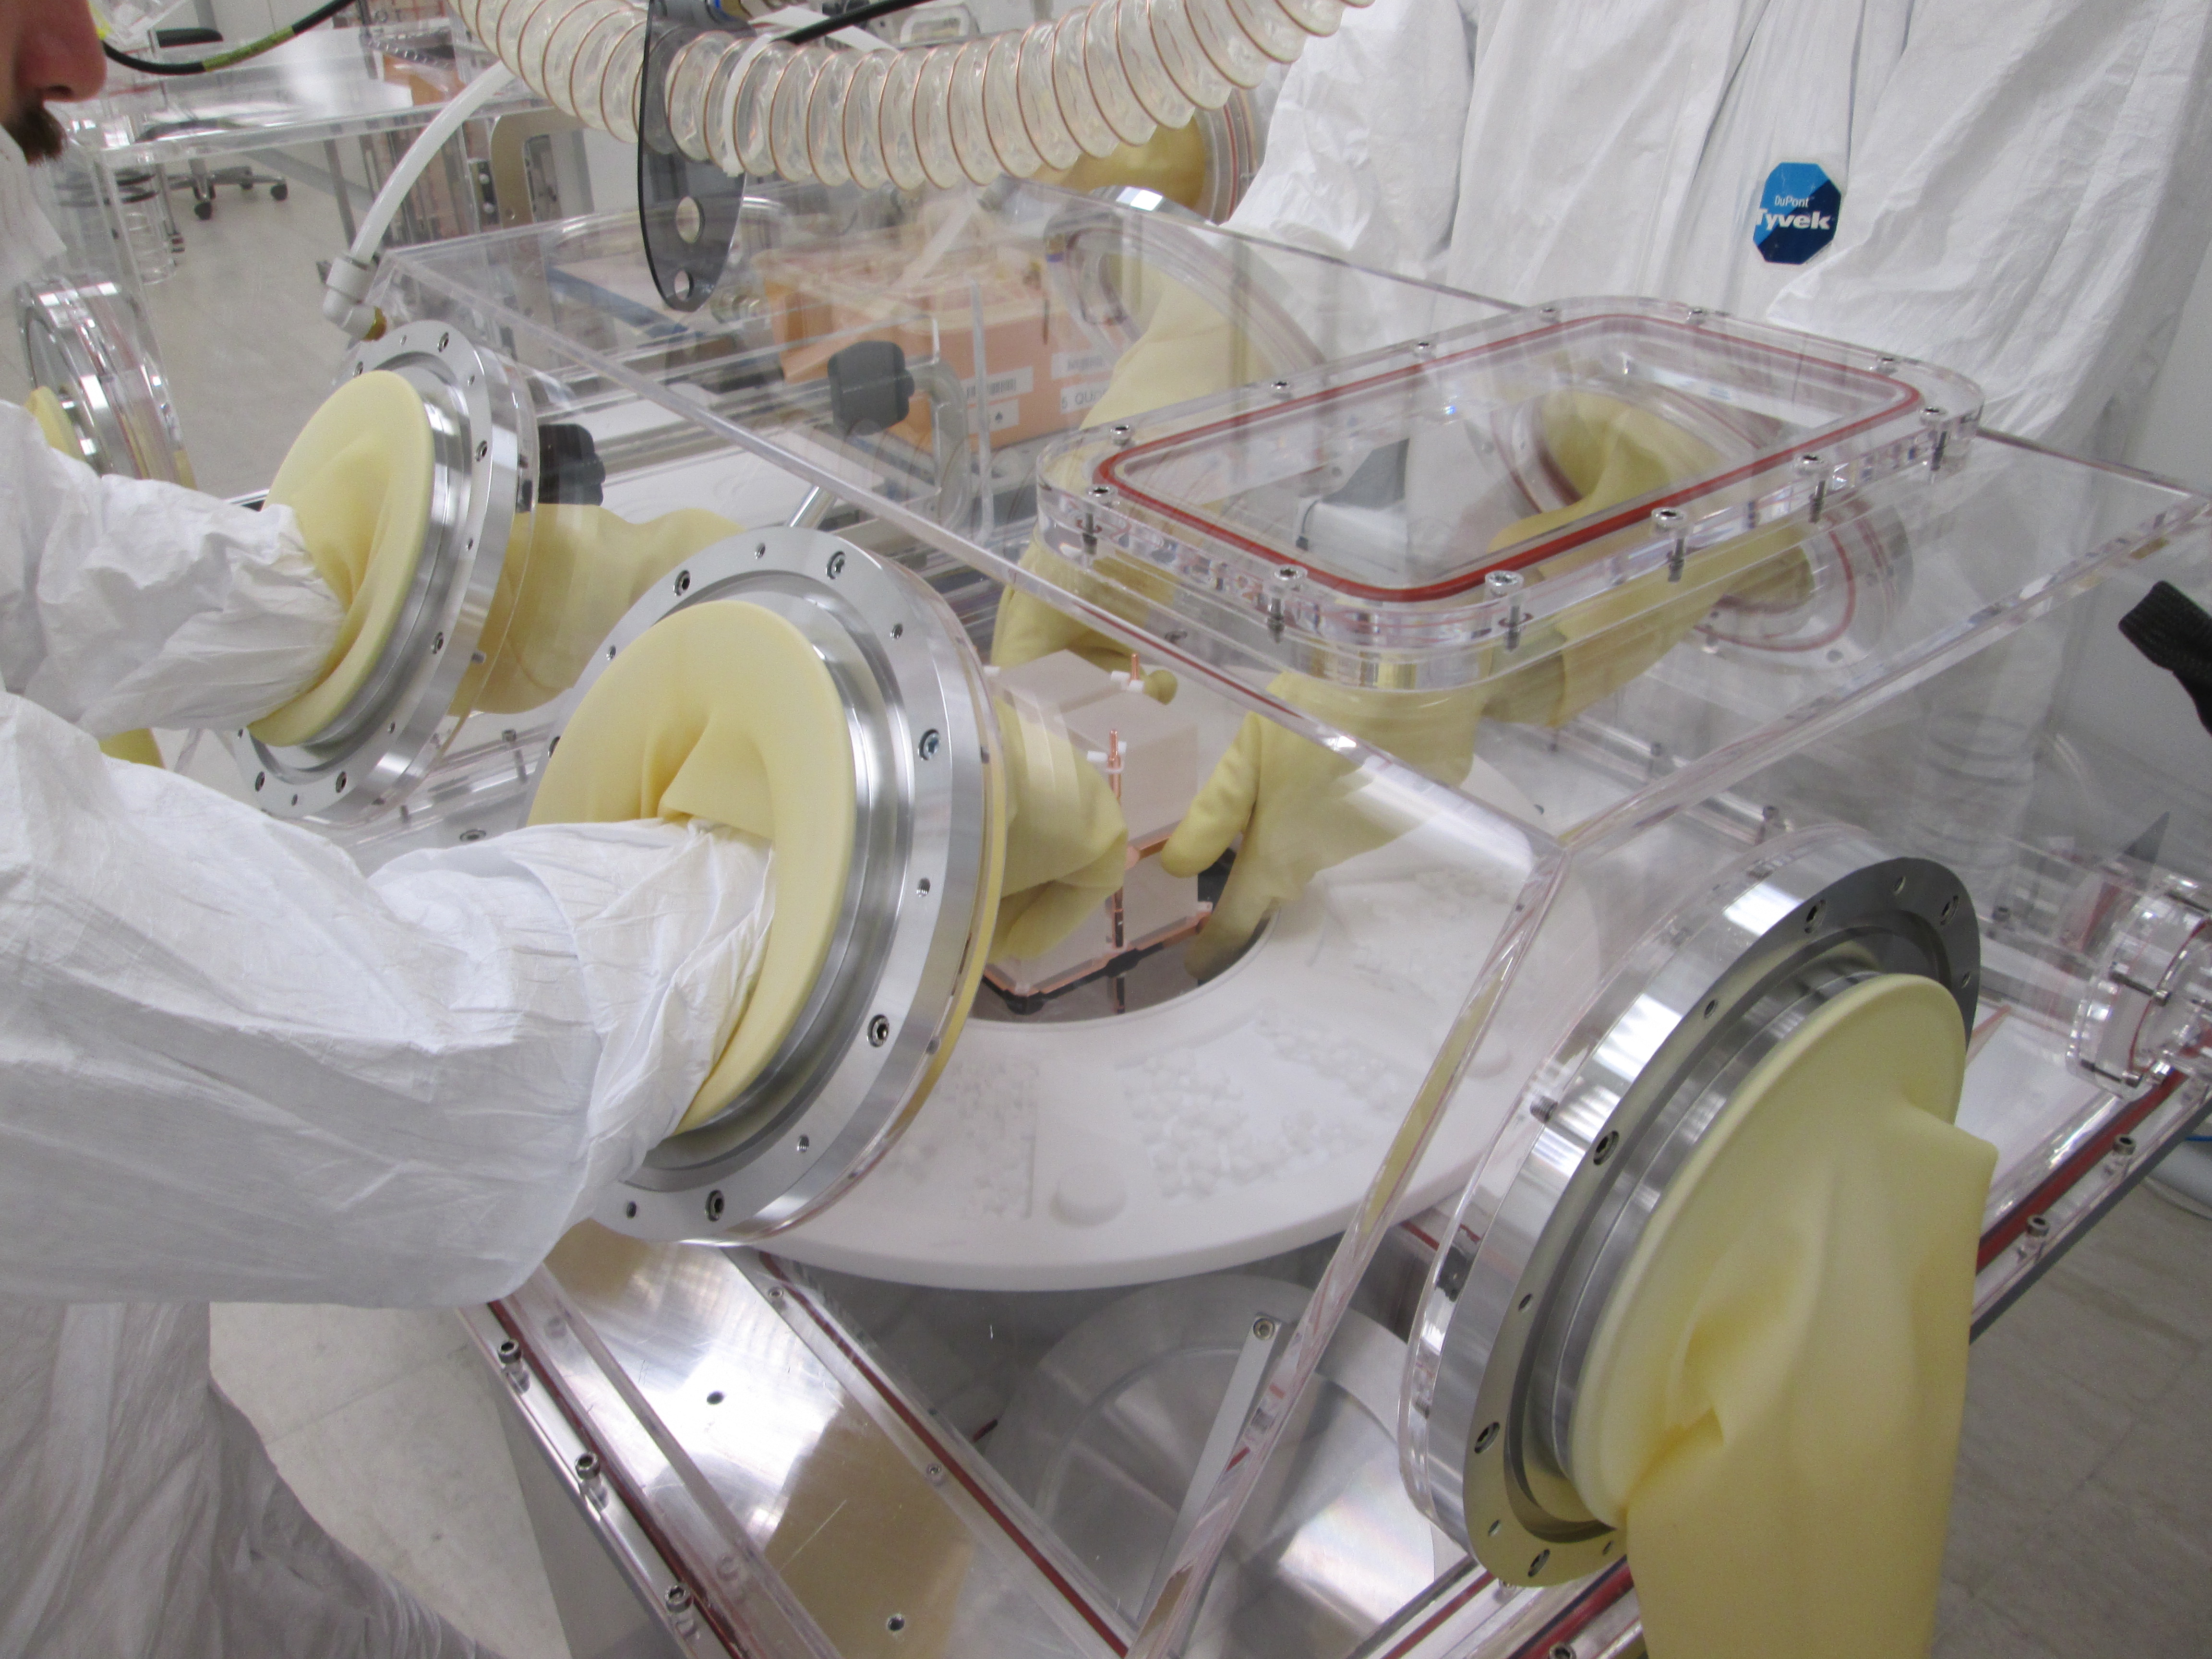
\includegraphics[width=0.6\linewidth]{Figures/TowerAssemblyBox.jpg}
    \caption[The glovebox used for tower assembly.]
    {The glovebox used for tower assembly.
    As each floor of the tower is completed, the tower is lowered into the garage.
    Once all 13 floors are assembled, the tower is sealed into the garage and the next glovebox is put into place above.
    Photograph courtesy of the CUORE collaboration.}
    \label{fig:assemblybox}
\end{figure}

The next part of the assembly is to attach the CuPEN tapes to the sides of the tower inside a larger glovebox.
The tapes are glued to the wire trays by means of Araldite Standard bicomponent epoxy\footnote{\RaggedRight\url{http://www.go-araldite.com/products/epoxy-adhesives/araldite-standard-2-x-15ml-tube}}.
The glovebox used for this procedure is shown in \autoref{fig:assemblybox_2}.
The wire trays are left open until the next step, the wire bonding of the chips to CuPEN tape, is completed.


\begin{figure}[htbp]
    \centering
    \includegraphics[width=0.6\linewidth, angle=90,origin=c]{Figures/TowerAssemblyBox_2.jpg}
    \caption[The assembly box used to assemble the CuPEN tapes on the towers.]
    {The assembly box used to assemble the CuPEN tapes on the towers.
    This assembly box is also flushed with nitrogen when a tower is in place, and the vertical access (in comparison with the box in \autoref{fig:assemblybox}) allows for placing the wire trays and tapes on the tower.
    The $\approx60~\textrm{cm}$ of tape is rolled up inside PTFE cylinders and can be seen at the top of the tower.
    Photograph courtesy of the CUORE collaboration.}
    \label{fig:assemblybox_2}
\end{figure}

The last step of the tower assembly process is the bonding of the gold wires to the copper pads on the tower.
This step is performed in the same glovebox as the previous step, but a modified Westbond 7700E manual wire bonder, mounted on rails and shown in \autoref{fig:bonding_machine}, is inserted on the right side of the glovebox.
With this bonder, the gold cables (4 for redundancy) are ball-bonded onto the chip pads and then wedge bonded to the copper pads on the CuPEN tape, as shown in \autoref{fig:bonds}.
Finally, another ball-bond is placed on the wedge bond to add extra security to the connection.
Considering the 988 crystals to be instrumented, and in line with the previous comments regarding the uniformity of the gluing, this process was also designed to be as repeatable as possible, and the lengths of the bonded gold wire are as uniform as possible.
After the tower assembly is completed, the towers are stored in nitrogen-flushed containers, shown in \autoref{fig:tower_storage}.

\begin{figure}[htbp]
    \centering
    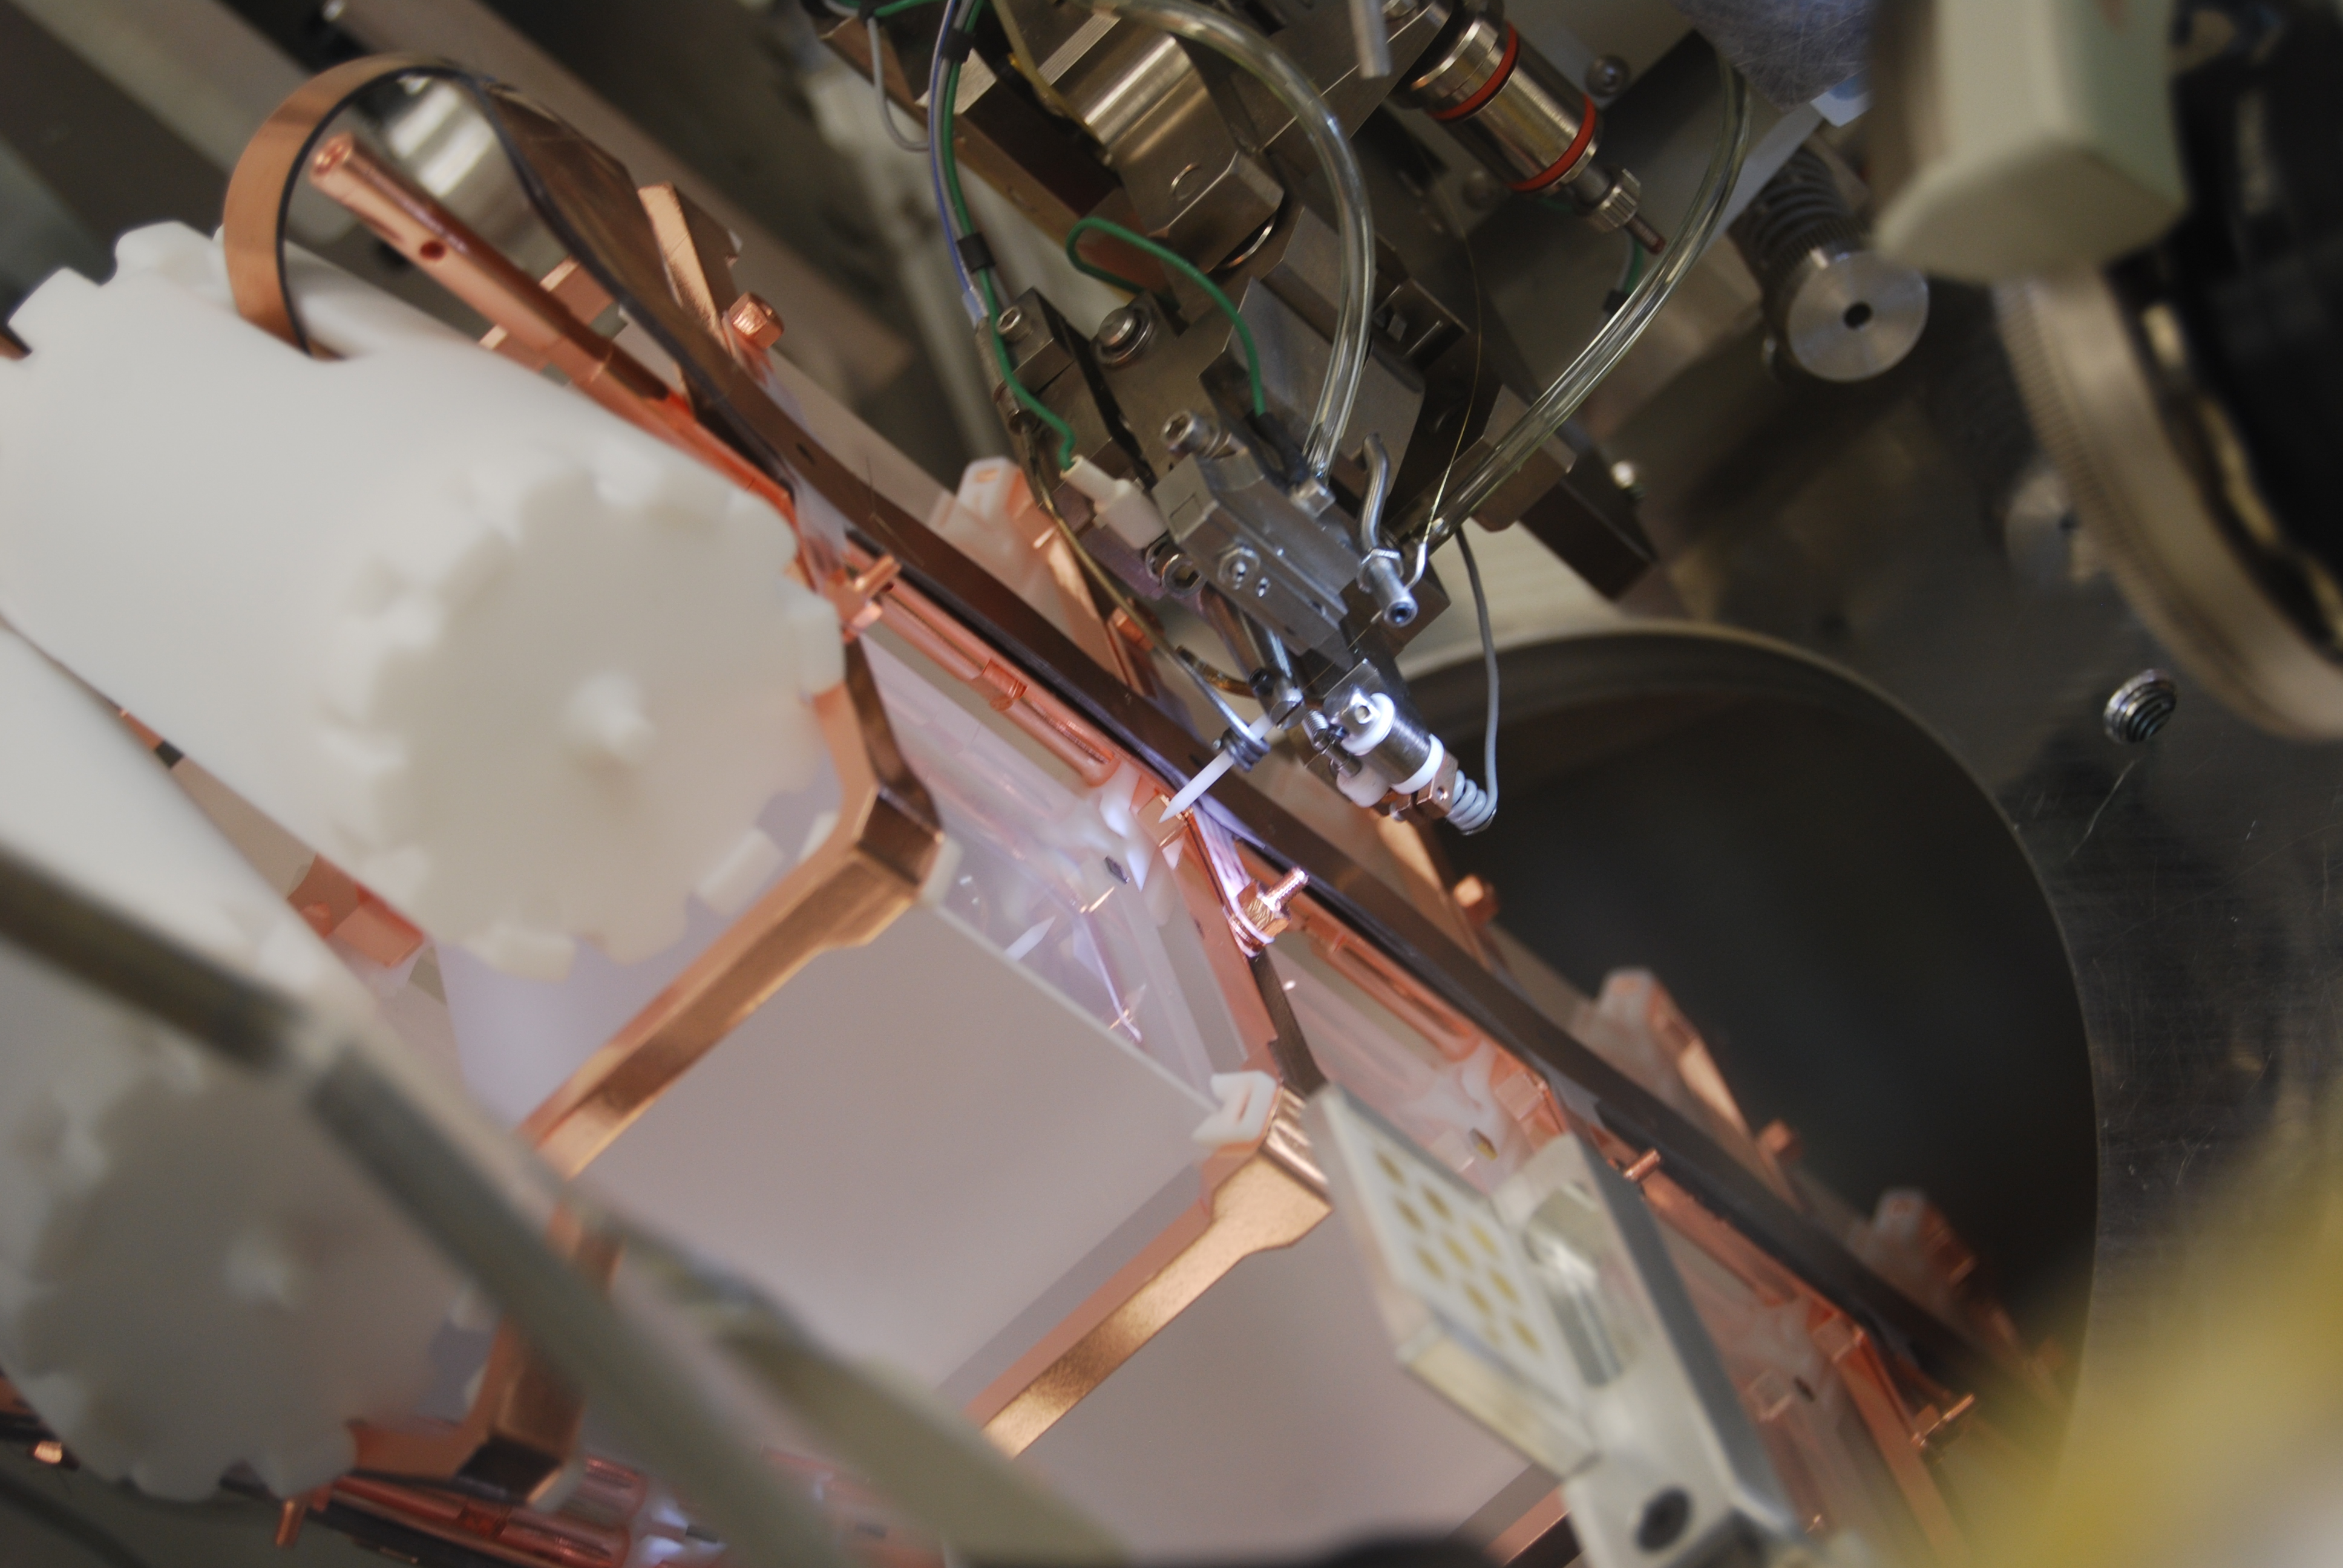
\includegraphics[width=0.6\linewidth, angle=270, origin=c]{Figures/bonding_machine.jpg}
    \caption[The wire bonding machine used in CUORE.]
    {The wire bonding machine used in CUORE.
    The bonder was modified to allow motion vertically and the rails serve to increase its reach.
    The tower is raised/lowered or rotated by a second operator, and a video camera with high magnification is used to make and verify the connections.
    Photograph courtesy of the CUORE collaboration.}
    \label{fig:bonding_machine}
\end{figure}

\begin{figure}[htbp]
    \centering
    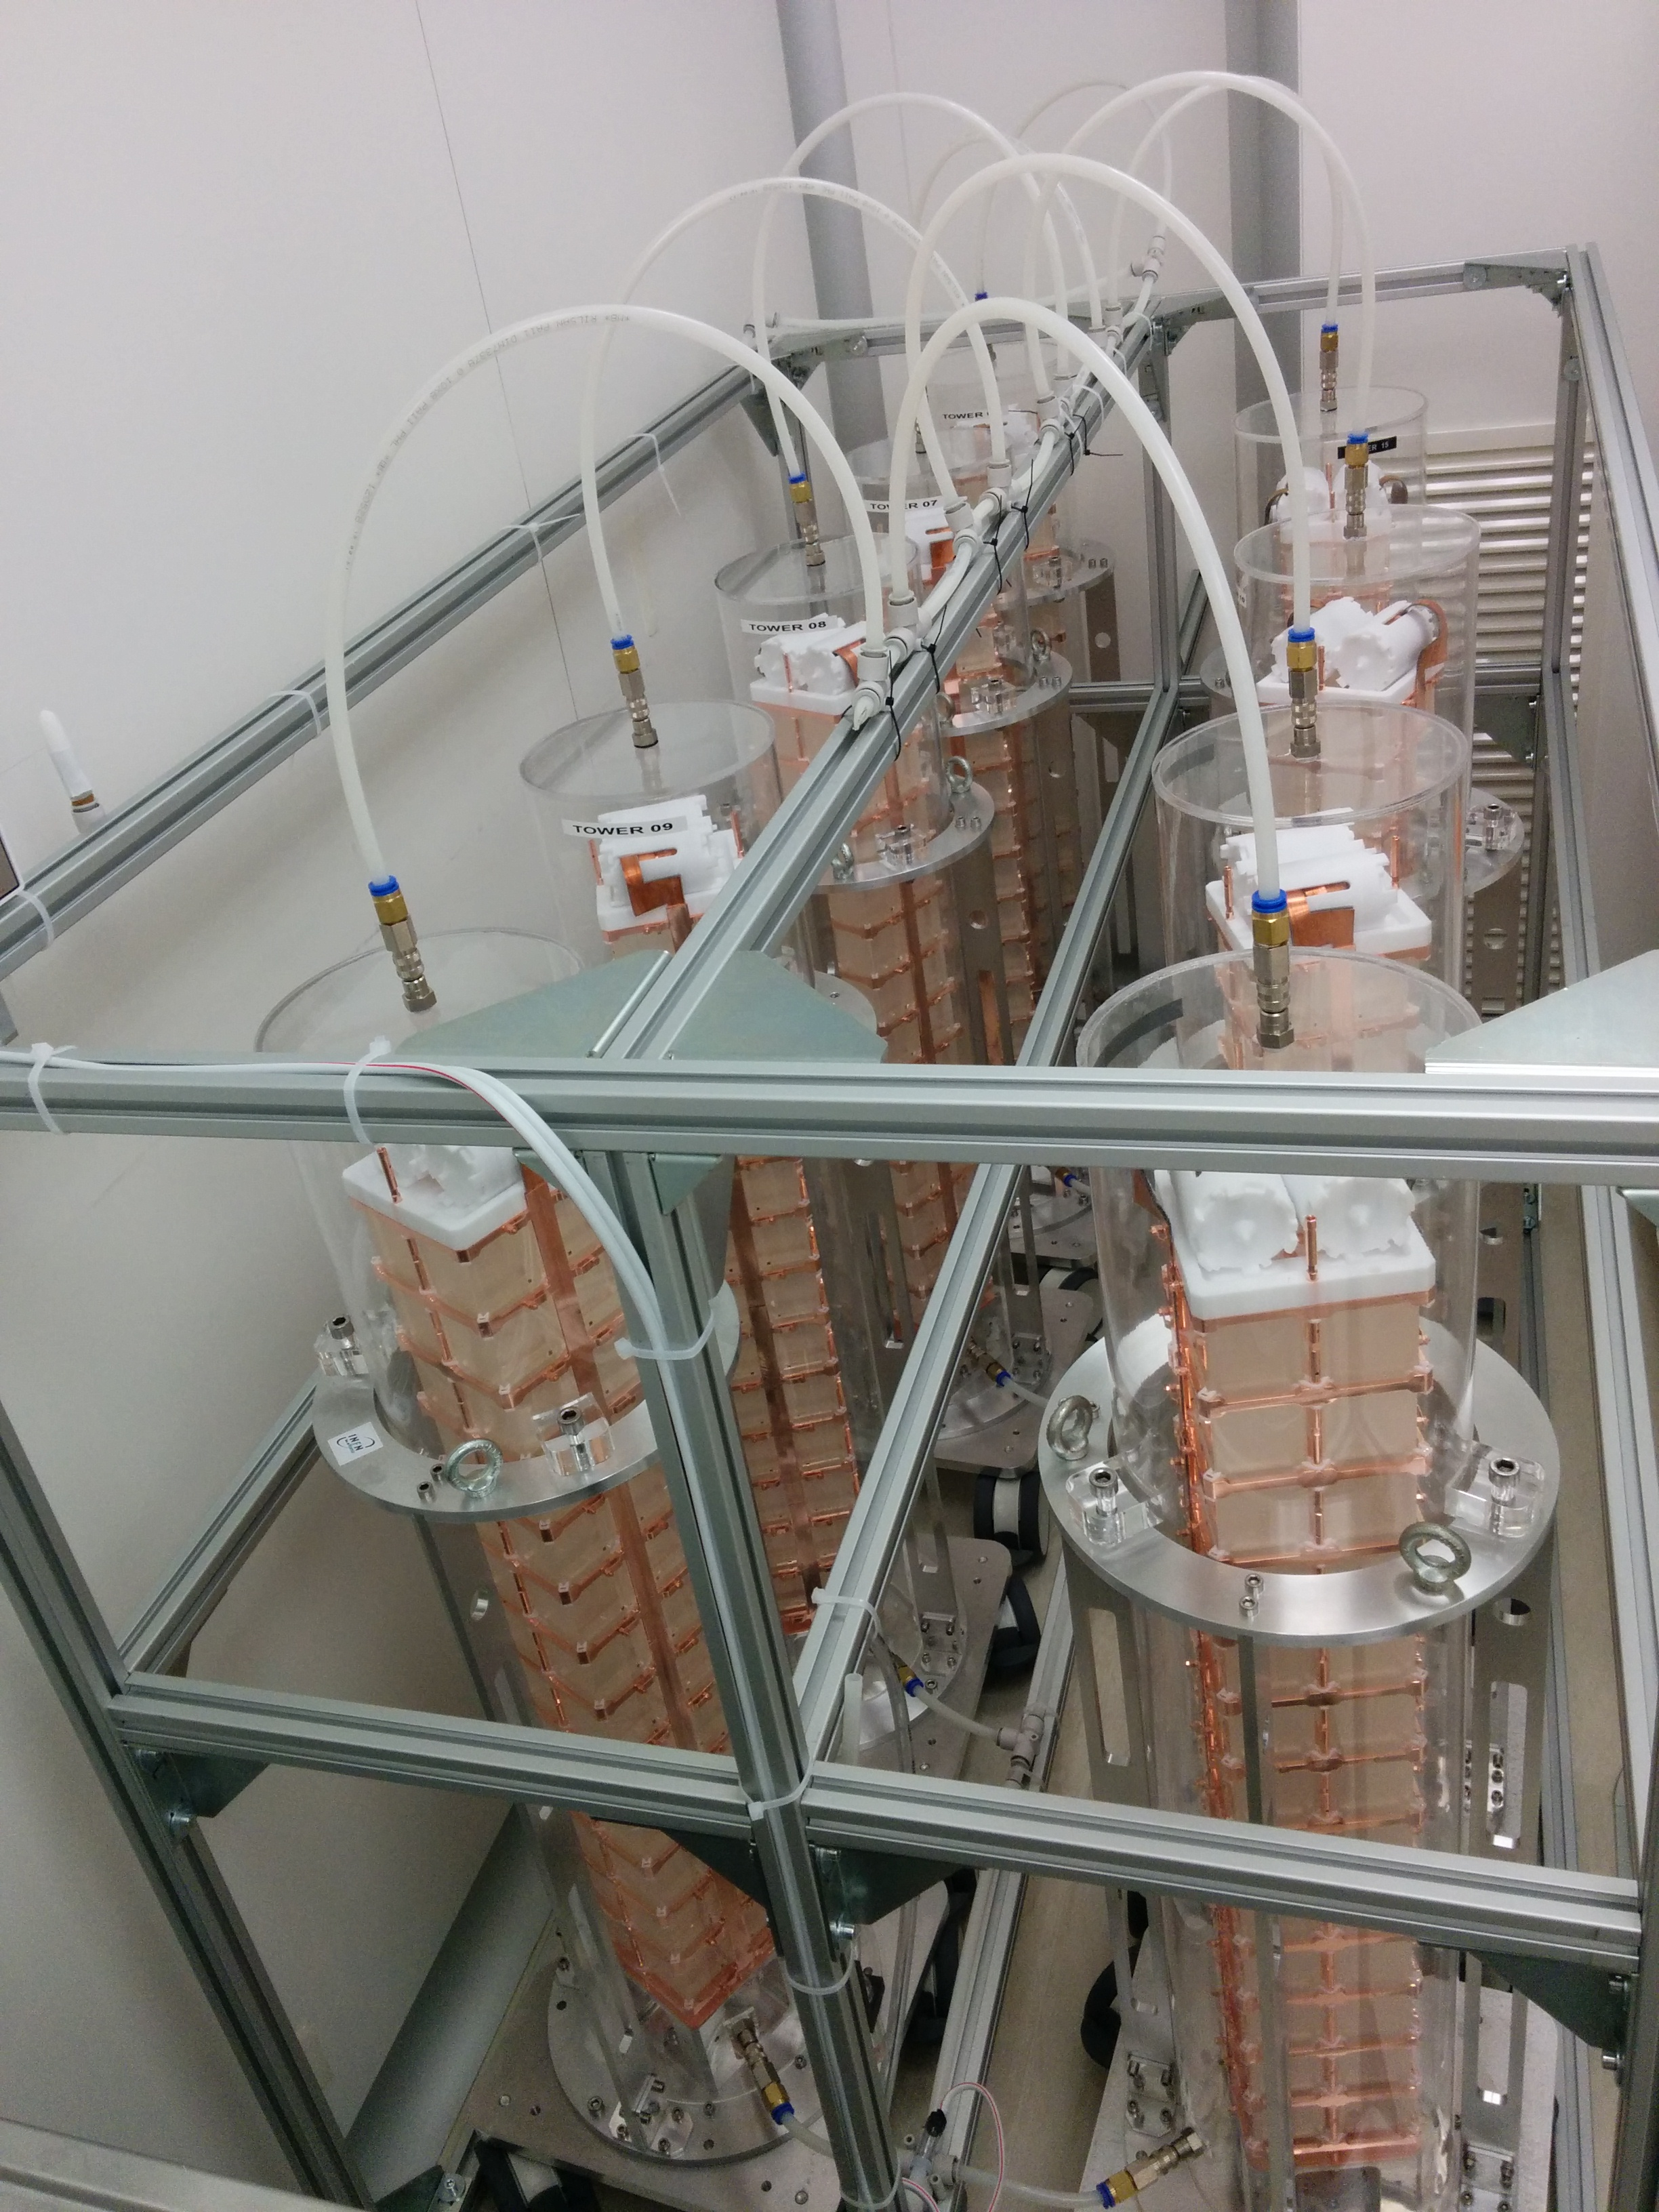
\includegraphics[width=0.5\linewidth]{Figures/cuore_towers_pic1.jpg}
    \caption[The storage area for the completed CUORE towers before installation.]
    {The storage area for the completed CUORE towers before installation.}
    \label{fig:tower_storage}
\end{figure}

\subsubsection{Tower Installation}
After the towers are completed and and the cryostat is ready for operation, the CUORE towers need to be installed into the cryostat.
This is another critical operation, as this is the first and only time that the CUORE crystals are exposed to air, with an approximate exposure of 1 day per tower.
In order to complete this activity, a specialized clean room was installed around the exposed inner part of the cryostat.
As the danger of being exposed to air is due to the presence of Radon in the air.
LNGS has an activity of 80 $\textrm{Bq}/\textrm{m}^3$ of Radon \cite{UndergroundLabs_Radon}, which required the use of a system to flush this specialized clean room with radon-free air.
This system reduced the radon to $<1~\textrm{Bq}/\textrm{m}^3$.
Each of the towers is then connected to the tower support plate independently, and the inner guide tubes for the DCS, discussed later in \autoref{chap:DCS}, are also connected at this time.
A view of the completed cryostat is shown in \autoref{fig:cuore_photograph}.


\begin{figure} [htbp]
    \centering
    \includegraphics[width=0.8\linewidth]{Figures/CUORE_29Aug16_HR-2477.jpg}
    \caption[A photograph of the 19 CUORE towers from below.
    Photo Credit: Yury Suvorov.]
    {A photograph of the 19 CUORE towers from below after installation in the cryostat.
    Also visible are the inner calibration source tubes with their PTFE caps.
    Photo Credit: Yury Suvorov.}
    \label{fig:cuore_photograph}
\end{figure}

\section{Predecessor Experiments}
\label{sec:Predecessor Experiments}
The CUORE experiment benefits from the experience gained through multiple previous incarnations of this bolometric technique in \teotwo.
Starting with the smallest proof-of-concept detectors, successive generations of this technology \cite{ }have increased in total detector mass and decreased in background in order to increase sensitivity and further probe \zeronubb~decay.
This almost-exponential growth in mass in the different generations of CUORE-like experiments from 73~g to 742~kg is shown in \autoref{fig:bolometer_mass_over_time}.
Of course, as shown in \autoref{eq:sensitivity_short}, the detector mass is only one part of the sensitivity equation, but successive experiments have also have significantly reduced backgrounds and other improvements to increase sensitivity beyond merely the increase from increased mass.
As a full description and history of the CUORE-like experiments is too long for discussion here, the most recent experiments, viz. Cuoricino and CUORE-0, that directly inform choices made for CUORE are described below.

\begin{figure}[htbp]
    \centering
    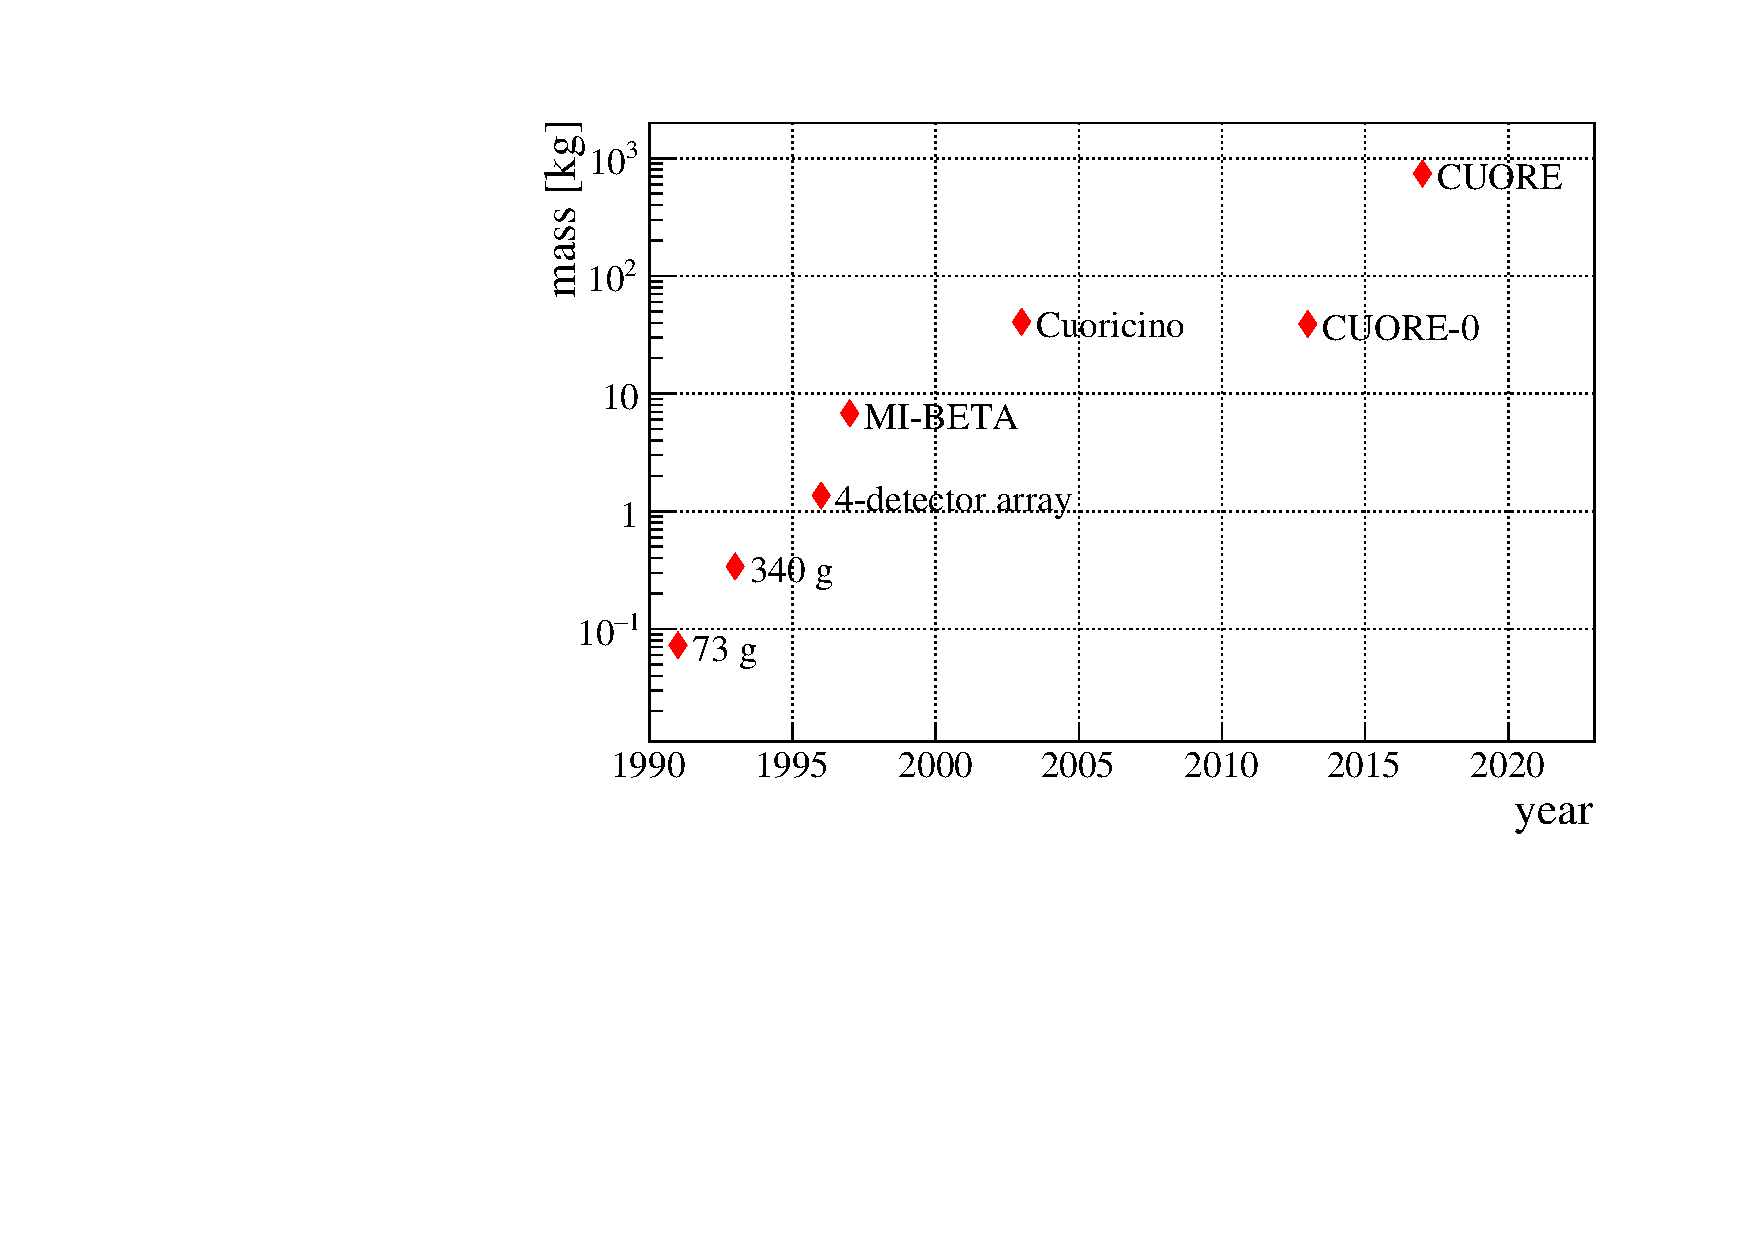
\includegraphics[width=\linewidth]{Figures/bolometer_mass_over_time.pdf}
    \caption[The increase in mass of \teotwo~crystals in successive experiments.]
    {The increase in mass of \teotwo~crystals in successive experiments.}
    \label{fig:bolometer_mass_over_time}
\end{figure}

\subsection{Cuoricino}
Building off the success of the Mi-Beta experiment \cite{Pirro:2002gw}, the Cuoricino experiment \cite{Andreotti:2010vj} performed a search of \zeronubb~with a tower consisting of 62 \teotwo~crystals, shown in \autoref{fig:Cuoricino_tower}, and, in addition, the Cuoricino experiment also served as a testing bed for CUORE.
Of the 62 crystals used in Cuoricino, 44 were ``big crystals" with $5\times5\times5~\textrm{cm}^3$ of naturally-abundant $^{130}$Te, 14 were ``small crystals" with $3\times3\times6~\textrm{cm}^3$ of naturally-abundant $^{130}$Te, 2 were the same size as the small crystals but with 75\% enriched $^{130}$Te, and the final 2 crystals were enriched with $^{128}$Te and had a negligible $^{130}$Te content.
In total, the crystals had a mass of $\approx11$ kg of $^{130}$Te and completed data-taking with 19.75 $\textrm{kg}\cdot \textrm{yr}$ of $^{130}$Te exposure.

\begin{figure}[htbp]
    \centering
    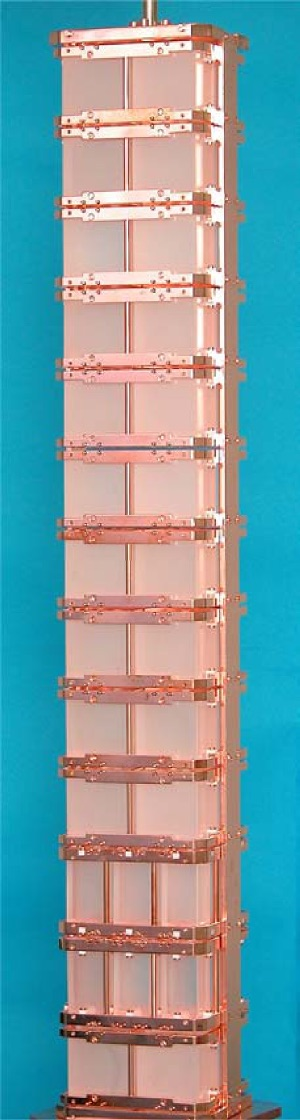
\includegraphics[width=0.8\linewidth, height=0.8\linewidth, keepaspectratio, angle=270, origin = c]{Figures/CUORICINO.jpg}
    \vspace*{-1.5 in}
    \caption[The Cuoricino tower consisting of both big crystals and small unenriched and enriched crystals.]
    {The Cuoricino tower (sideways, with bottom at left) consisting of both big crystals and small unenriched and enriched crystals.}
    \label{fig:Cuoricino_tower}
\end{figure}

With this exposure, Cuoricino determined an experimental limit of $2.8\times10^{25}$ yr (90\% C.L).
During the operation of Cuoricino, a few things were learned that influenced the design choices in CUORE.
As the big crystals with naturally abundant $^{130}$Te had better energy resolution ($6.3 \pm2.5$ keV) than the smaller unenriched ($9.9\pm4.2$ keV) and enriched crystals ($13.9\pm5.3$ keV), the big crystals were selected as the choice for CUORE.
With this resolution for the big crystals, the design goal of the CUORE crystals was set to be 5 keV, and the improved wire bonding method described in \autoref{ssec:Tower Assembly} was developed in order to attain this.
Cuoricino's cryostat was a wet dilution refrigerator that required a liquid helium bath to be refilled every 48 hours, which interrupted data-taking for 3-4 hours at a time.
As this directly affects the detector livetime and stability, CUORE's cryostat is designed as a dry cryostat and makes use of pulse tube cooling at the 4-K stage.
Lastly, as $\alpha$ backgrounds made up a significant portion of the background of Cuoricino in the region of interest, a more rigorous parts selection and cleaning regimen was undertaken for CUORE, which is described in detail in \autoref{ssec:Parts Selection and Cleaning}.

\begin{figure}[htbp]
    \centering
    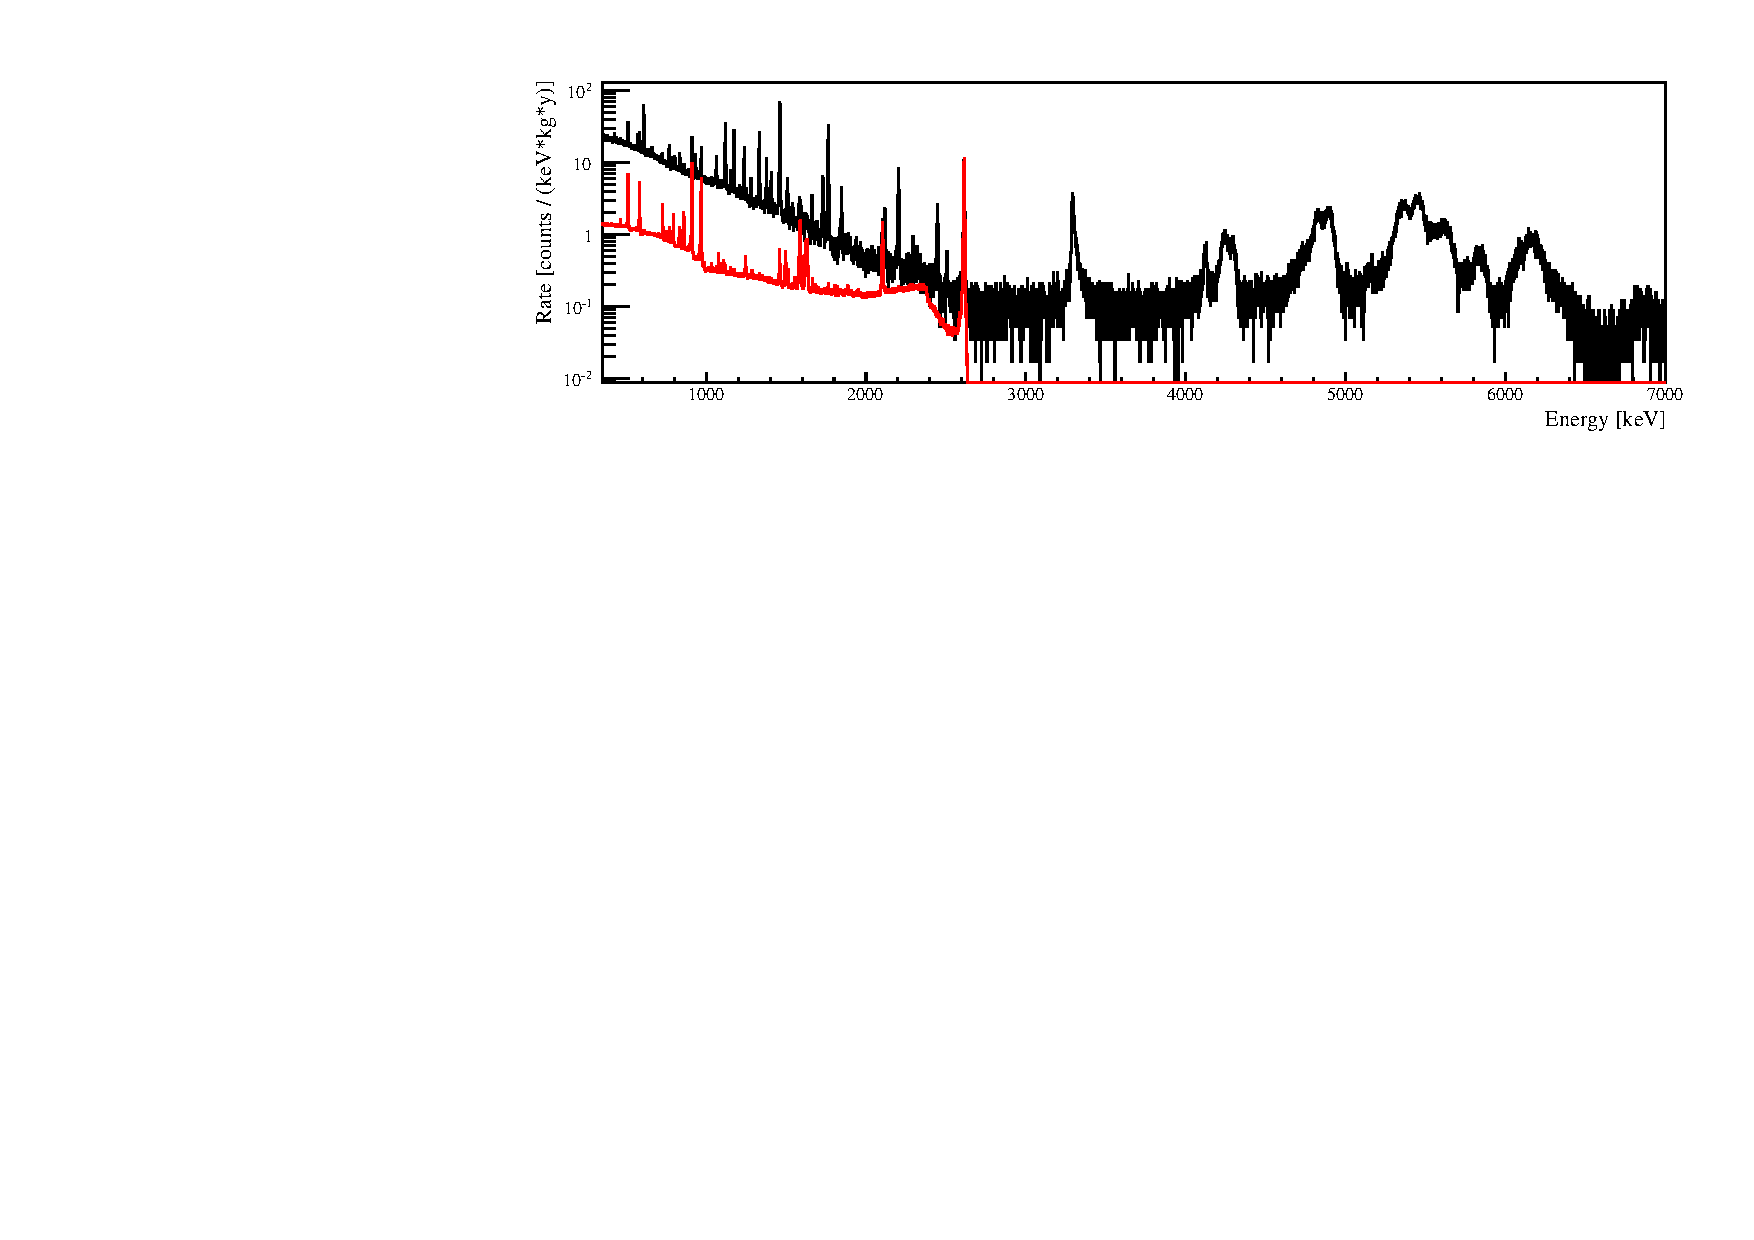
\includegraphics[width=0.8\linewidth]{Figures/CuoricinoSpectrum.pdf}
    \caption[The energy spectrum for Cuoricino in background (black) data along with calibration (red) data which has been normalized to the 2615 keV peak.]
    {The energy spectrum for Cuoricino in background (black) data along with calibration (red) data which has been normalized to the 2615 keV peak.
    The calibration spectrum is normalized to highlight the difference between the background near the 2528 keV Q-value of \zeronubb~due to gammas depositing energy versus that of degraded alphas.}
    \label{fig:cuoricino spectrum}
\end{figure}

\subsection{CUORE-0}
\label{ssec:CUORE-0}

After the completion of the Cuoricino experiment, an intermediate experiment, CUORE-0, was planned while working on completing the CUORE cryostat.
CUORE-0 was meant to bridge the gap between Cuoricino and CUORE by installing a single CUORE-like tower into the Cuoricino cryostat.
In this way, a CUORE-like tower could be studied inside the well-understood Cuoricino cryostat which allowed the changes to the tower to be decoupled from changes to the cryostat.
A schematic of the experimental apparatus can be seen in \autoref{fig:CUORE-0_cryostat_schematic}.

\begin{figure} [htbp]
    \centering
    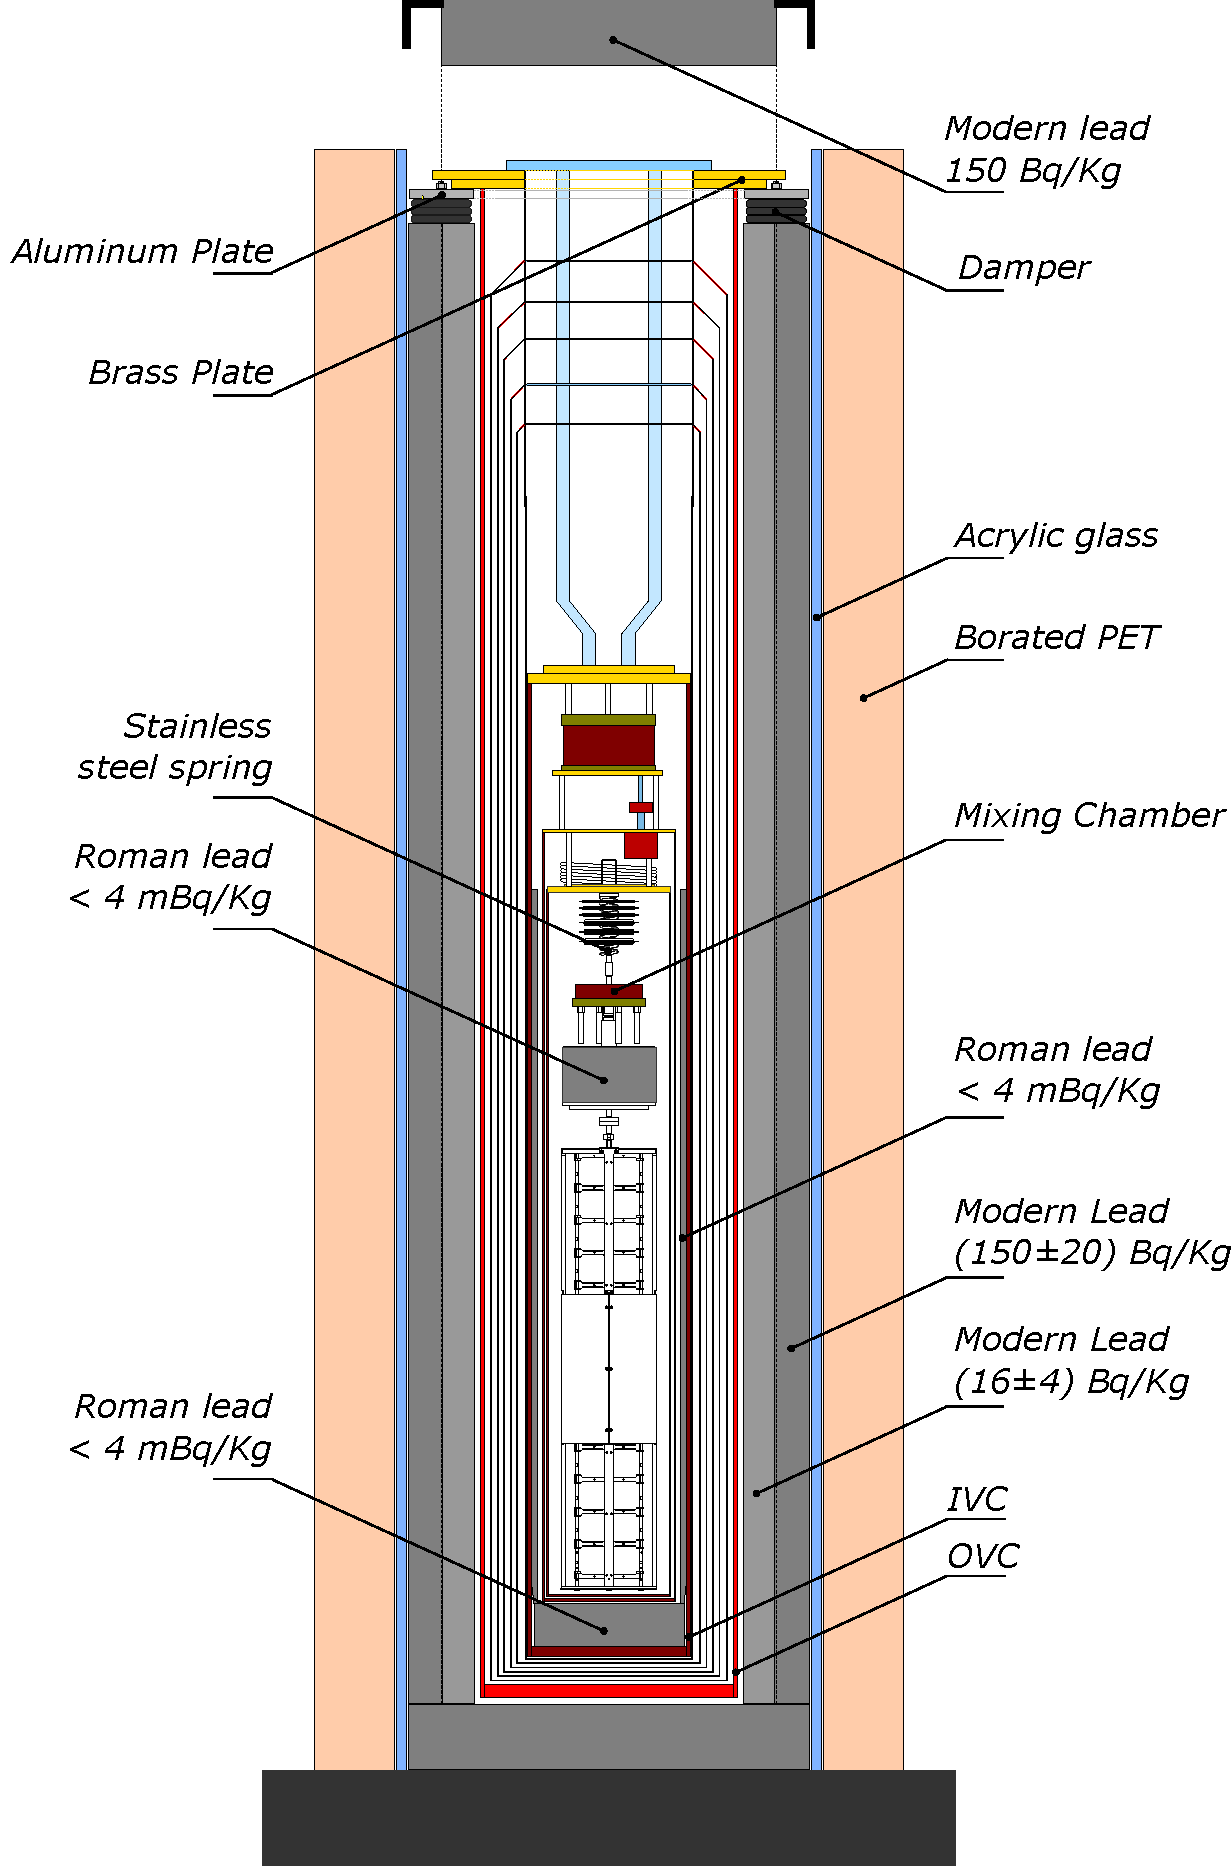
\includegraphics[width=0.8\linewidth]{Figures/CUORE-0_cryostat_schematic.pdf}
    \caption[A schematic of the CUORE-0 experiment.]
    {A schematic of the CUORE-0 experiment in the Cuoricino cryostat (not to scale).
    The CUORE-0 tower is in the center of the cryostat, and the calibration sources are deployed between the OVC and the external lead shield.}
    \label{fig:CUORE-0_cryostat_schematic}
\end{figure}

The purpose of this experiment, besides  making a measurement of \zeronubb, was to validate the improved materials selection and cleaning of the CUORE crystals.
This improvement is quantified in \autoref{fig:cuore-0_vs_cuoricino} where a signficant decease is observed in the \alpha~backgrounds which are due to components nearest to the crystals.
The \gamma~backgrounds are not reduced as significantly as the cryostat is the same between the CUORE and Cuoricino experiments.

\begin{figure}[htpb]
    \centering
    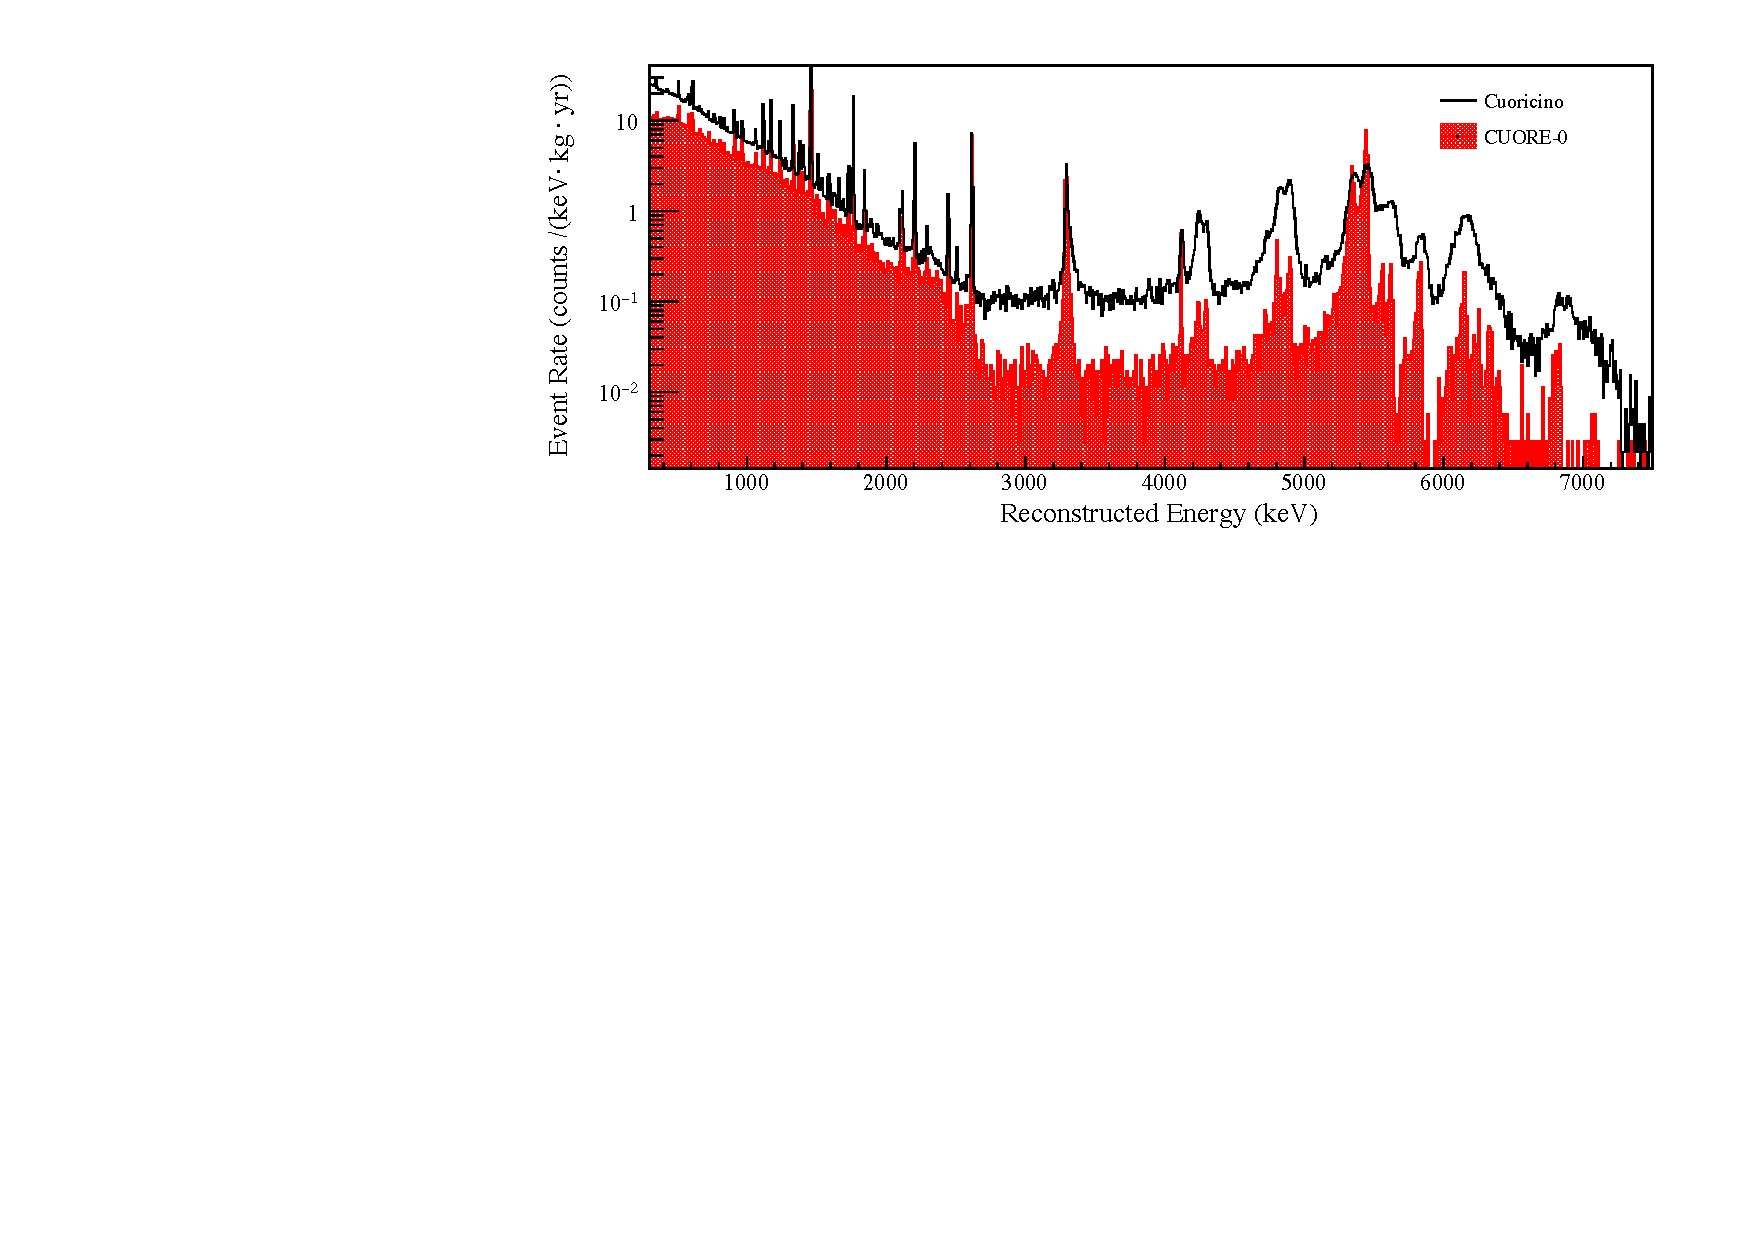
\includegraphics[width=\linewidth]{Figures/CUORE-0_vs_Cuoricino.pdf}
    \caption[A comparison of the backgrounds in the Cuoricino and CUORE-0 exeperiments.]
    {A comparison of the backgrounds in the Cuoricino and CUORE-0 experiments.
    The backgrounds are significantly reduced in the \gamma~ regions as the improved materials selection and cleaning procedures reduced the surface contaminants on the \teotwo~crystals and the copper frames on the tower.
    There is also some improvement on the level of \gamma~ backgrounds, but as the cryostat is the same, those contaminations remain.
    However, one peak in the $\alpha$ region from $^{210}$Po does not decrease, and may be particular to this single tower.}
    \label{fig:cuore-0_vs_cuoricino}
\end{figure}

CUORE-0 collected data between 2013 and 2015, and during this time many analysis and data-collection techniques were refined and improved for use in CUORE.
In particular, from the data collected, CUORE-0 was able to make the most precise measurement of \twonubb~decay in $^{130}$Te at the time, listed in \autoref{tab:2nuHalfLife} \cite{Alduino:2016vtd}.
In addition, CUORE-0 also performed a search for \zeronubb~and, in a combined analysis with the Cuoricino experiment, formed the most stringent limit at the time for \zeronubb~decay in $^{130}$Te with a limit of $T^{0ν}_{1/2}>4.0\times10^{24}$ yr \cite{Alfonso:2015wka}.

\section{CUORE Cryostat}
\label{sec:CUORE Cryostat}

Since the heat capacity of the CUORE crystals is so strongly dependent on temperature, it is critically important to have a system that can cool down the crystals to a base temperature of $\sim10$ mK and operate in a stable condition over long periods, up to CUORE's 5-year planned livetime.
To this end, a cryogen-free custom cryostat was constructed to house the crystals, shown in \autoref{fig:cryostat_cad_cutout} \cite{cryostat_commissioning}.
The cooling components of the cryostat are pulse tubes that cool the cryostat stages at 40-K\footnote{Naming convention: I use ``40-K" to denote cryostat stages and ``40 K" to denote temperatures.} and 4-K and a dilution refrigerator that is responsible for maintaining the coldest regions of the cryostat, including the crystals inside the 10-mK stage.
In addition to cooling the crystals, the cryostat also houses the shielding for the crystals such as the internal and, since this is a low-background experiment, is made of radiopure materials, especially near the detectors themselves.
Due to the background requirements and because the crystals themselves are housed inside the 10-mK shield, the cryostat was assembled underground at LNGS inside of a clean room.
Inside the cryostat, there are two vacuum volumes, the Outer Vacuum Chamber (OVC) and the Inner Vacuum Chamber (IVC).
The OVC consists of all the volumes outside of the 4-K stage, and is isolated from the IVC, which consists of all the volumes inside the 4-K stage, including the detectors.

\begin{figure}[htbp]
\centering
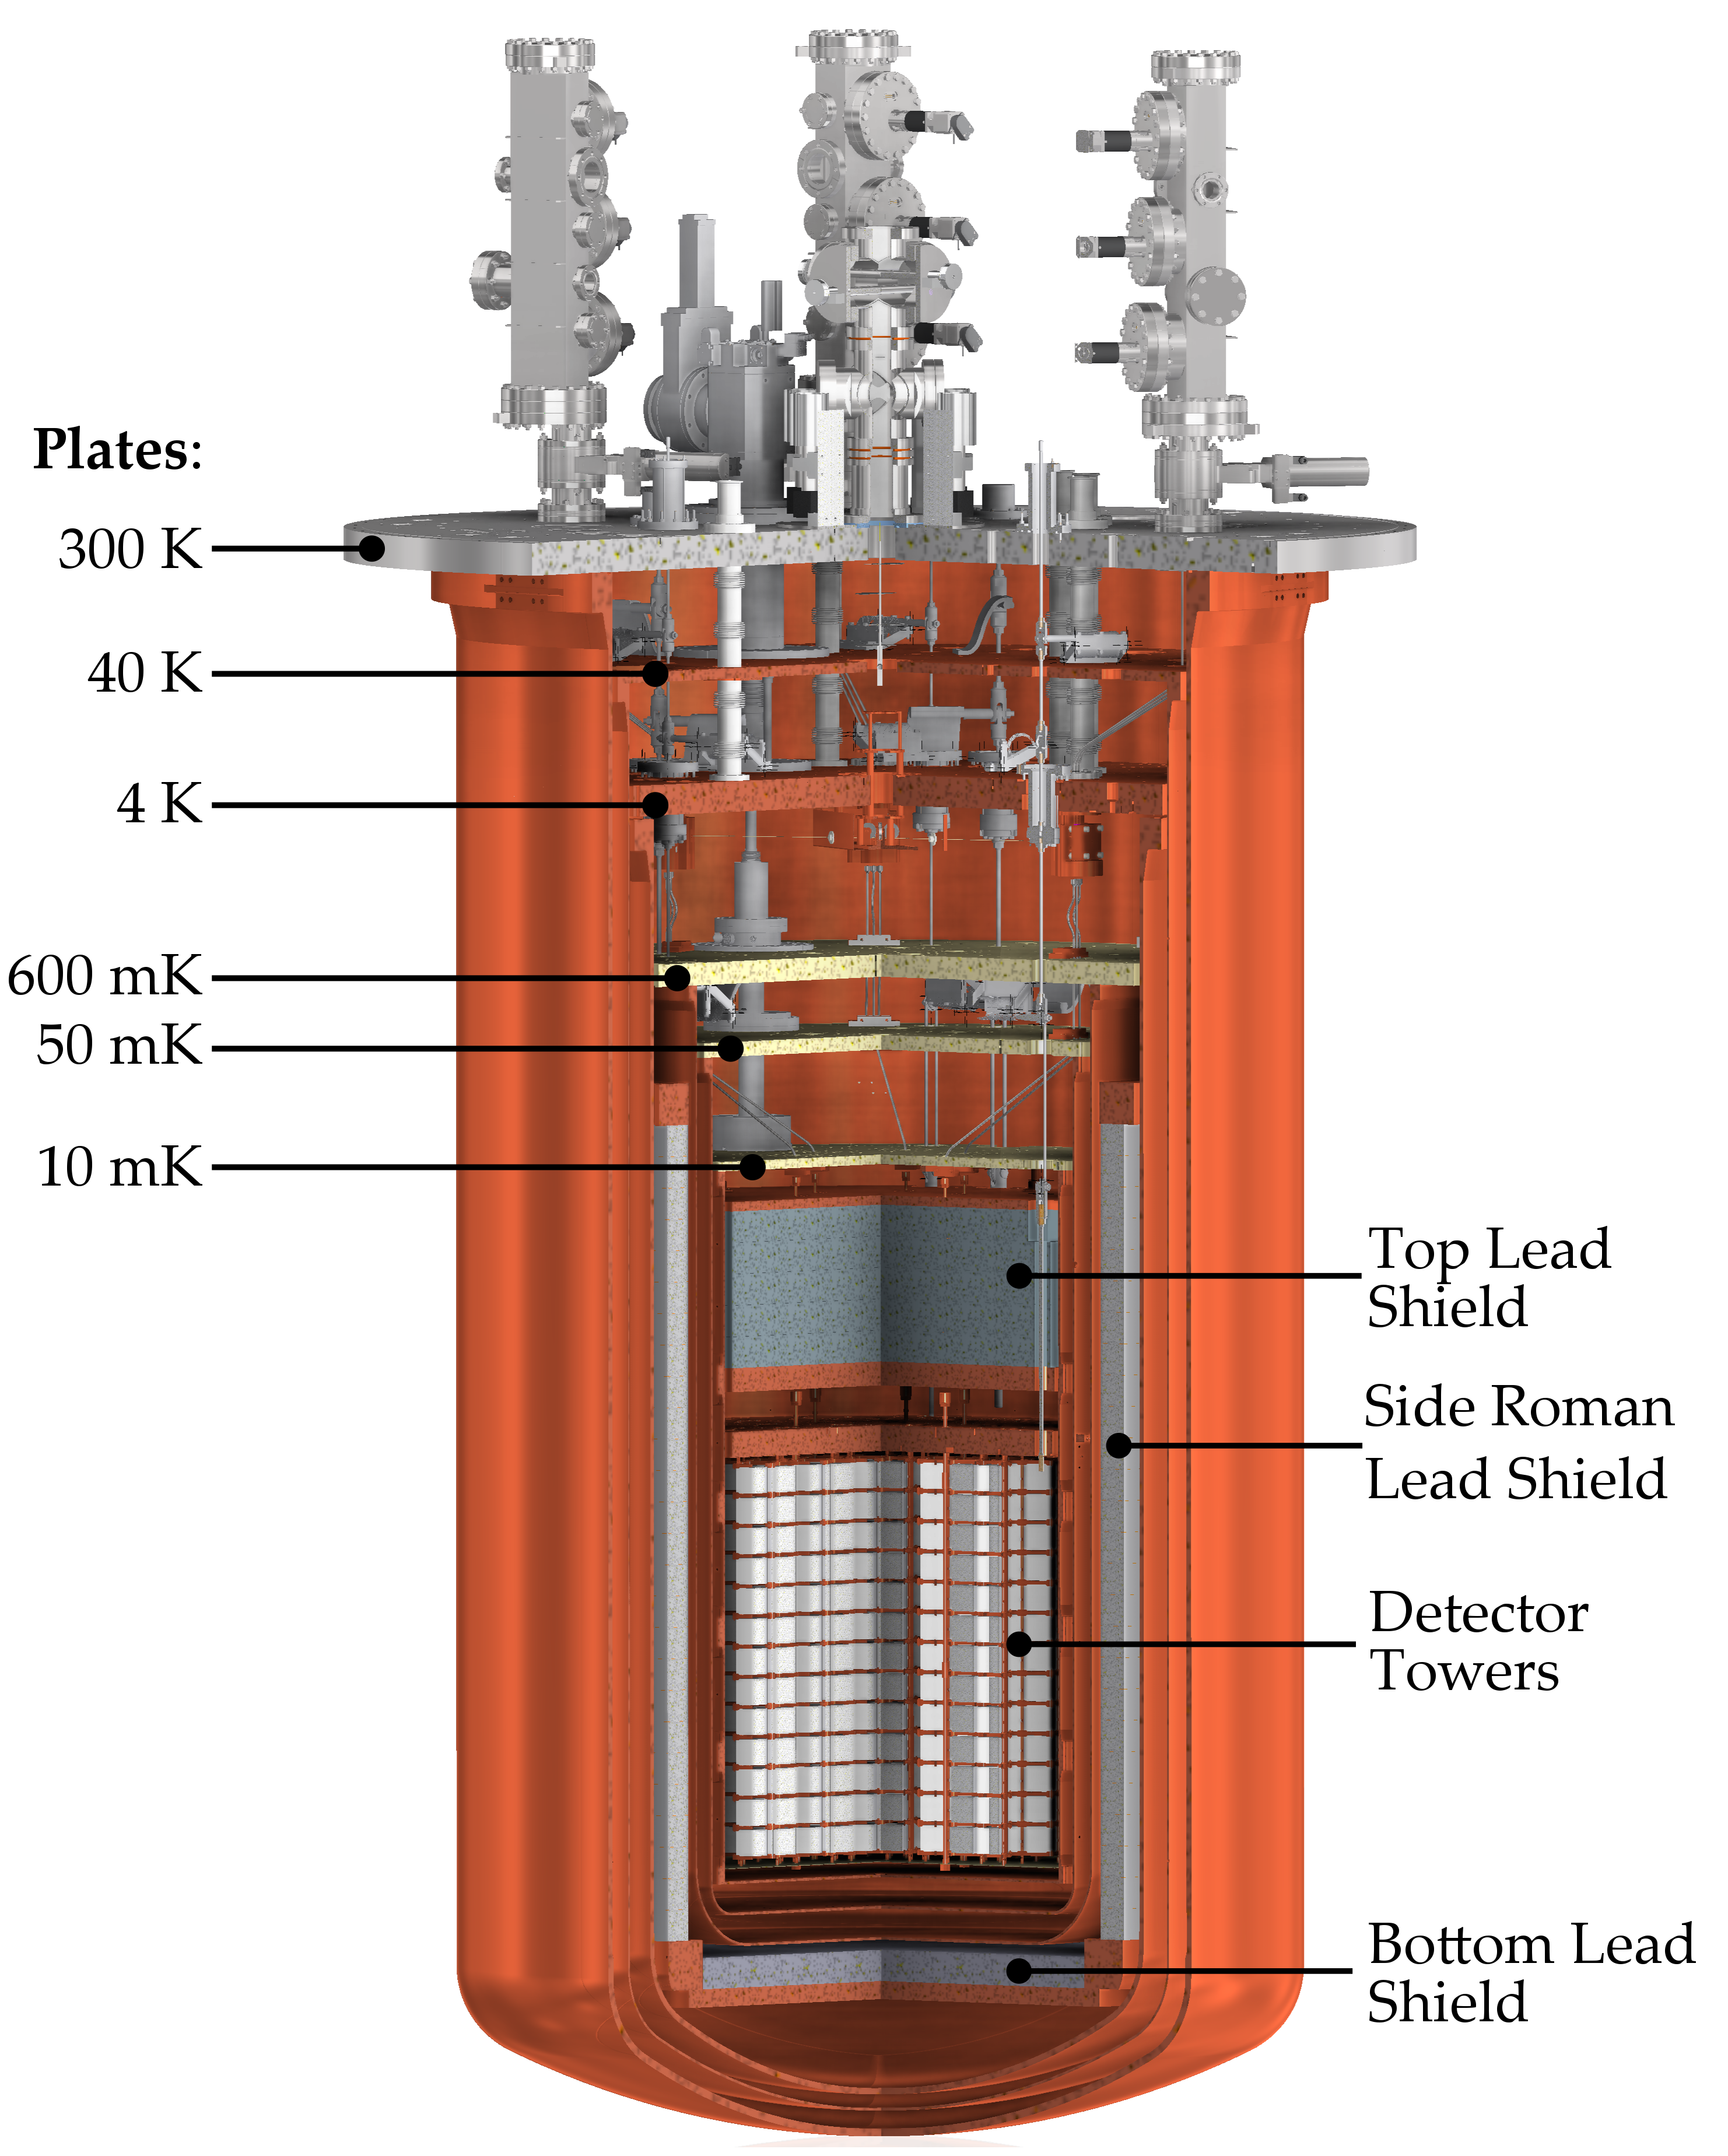
\includegraphics[width=\linewidth]{Figures/cryostat_Adjusted.png}
\caption[CAD cutaway of the CUORE cryostat.]
{A CAD drawing of a cutaway the CUORE cryostat showing the internal shielding of the cryostat.
The temperature stages of the cryostat are also shown.
Not included are the external shields which extend around the sides of the cryostat, shown in \autoref{fig:external_shielding}.
Figure courtesy of the CUORE collaboration.}
\label{fig:cryostat_cad_cutout}
\end{figure}

\subsubsection*{Detector Shielding and Vibration Isolation}
As noted above, the detectors need to be shielded from the environment and even from radioactivity in the shielding itself.
Starting from the outside of the experiment, shown in \autoref{fig:external_shielding}, there is an external lead shield with a layer of polyethylene and boric acid that surrounds the cryostat.
This $\sim70$ ton, 25 cm thick lead shielding acts to shield from the environmental gammas from LNGS, and the 18 cm thick polyethlene and 2 cm thick boric acid (H$_3$BO$_3$ powder) thermalize and absorb environmental neutrons.
This external shielding can be raised and lowered as needed, and remains lowered while working on the cryostat, and raised during physics data-taking.
Inside this external shielding is the cryostat, suspended from the main support plate above by three steel ropes.
This plate is supported by sand-filled columns, resting on rubber dampeners which act to seismically isolate the main support plate, and thus the cryostat) from the ground.
This is a particularly important component given the seismic nature of the area around LNGS as vibrations contribute to low-frequency noise in CUORE, as, at the low temperatures of CUORE, the frictive heating from motion of the cryostat affects the sensitivity of the CUORE bolometers.
In fact, even despite all these components, we set bad intervals, \color{red} discussed later in subsubsection bad intervals \color{black} during particularly intense seismic events around the globe.
At the top of the cryostat, the 300-K plate supports the 40-K, 4-K, and 600-mK plates by segmented steel rods.
Each of these plates also holds a corresponding cylindrical vessel that surrounds the inner vessels.
In addition, these vessels act as a radiation shield, both for thermal and particle radiation \color{red} better wording here? \color{black}.
In order to minimize the radioactivity of these components, with over 7 tonnes of mass, these plates and vessels are made of Oxygen-Free Electronic (OFE) copper (99.99\% Cu), with the exception of the 300-K plate and the top of the 300-K vessel which is made of the stronger austenitic stainless steel due to the load it carries. This radioactivity constraint carries over to the superinsulation used to cover the 40-K and 4-K stages of the cryostat, which is needed to reduce the thermal radiation heat load on the vessels, and was optimized for a choice of 17 kg in 30 and 10 layers of aluminized mylar and polyester foil for the 40-K and 4-K stages, respectively.

\begin{figure}
    \centering
    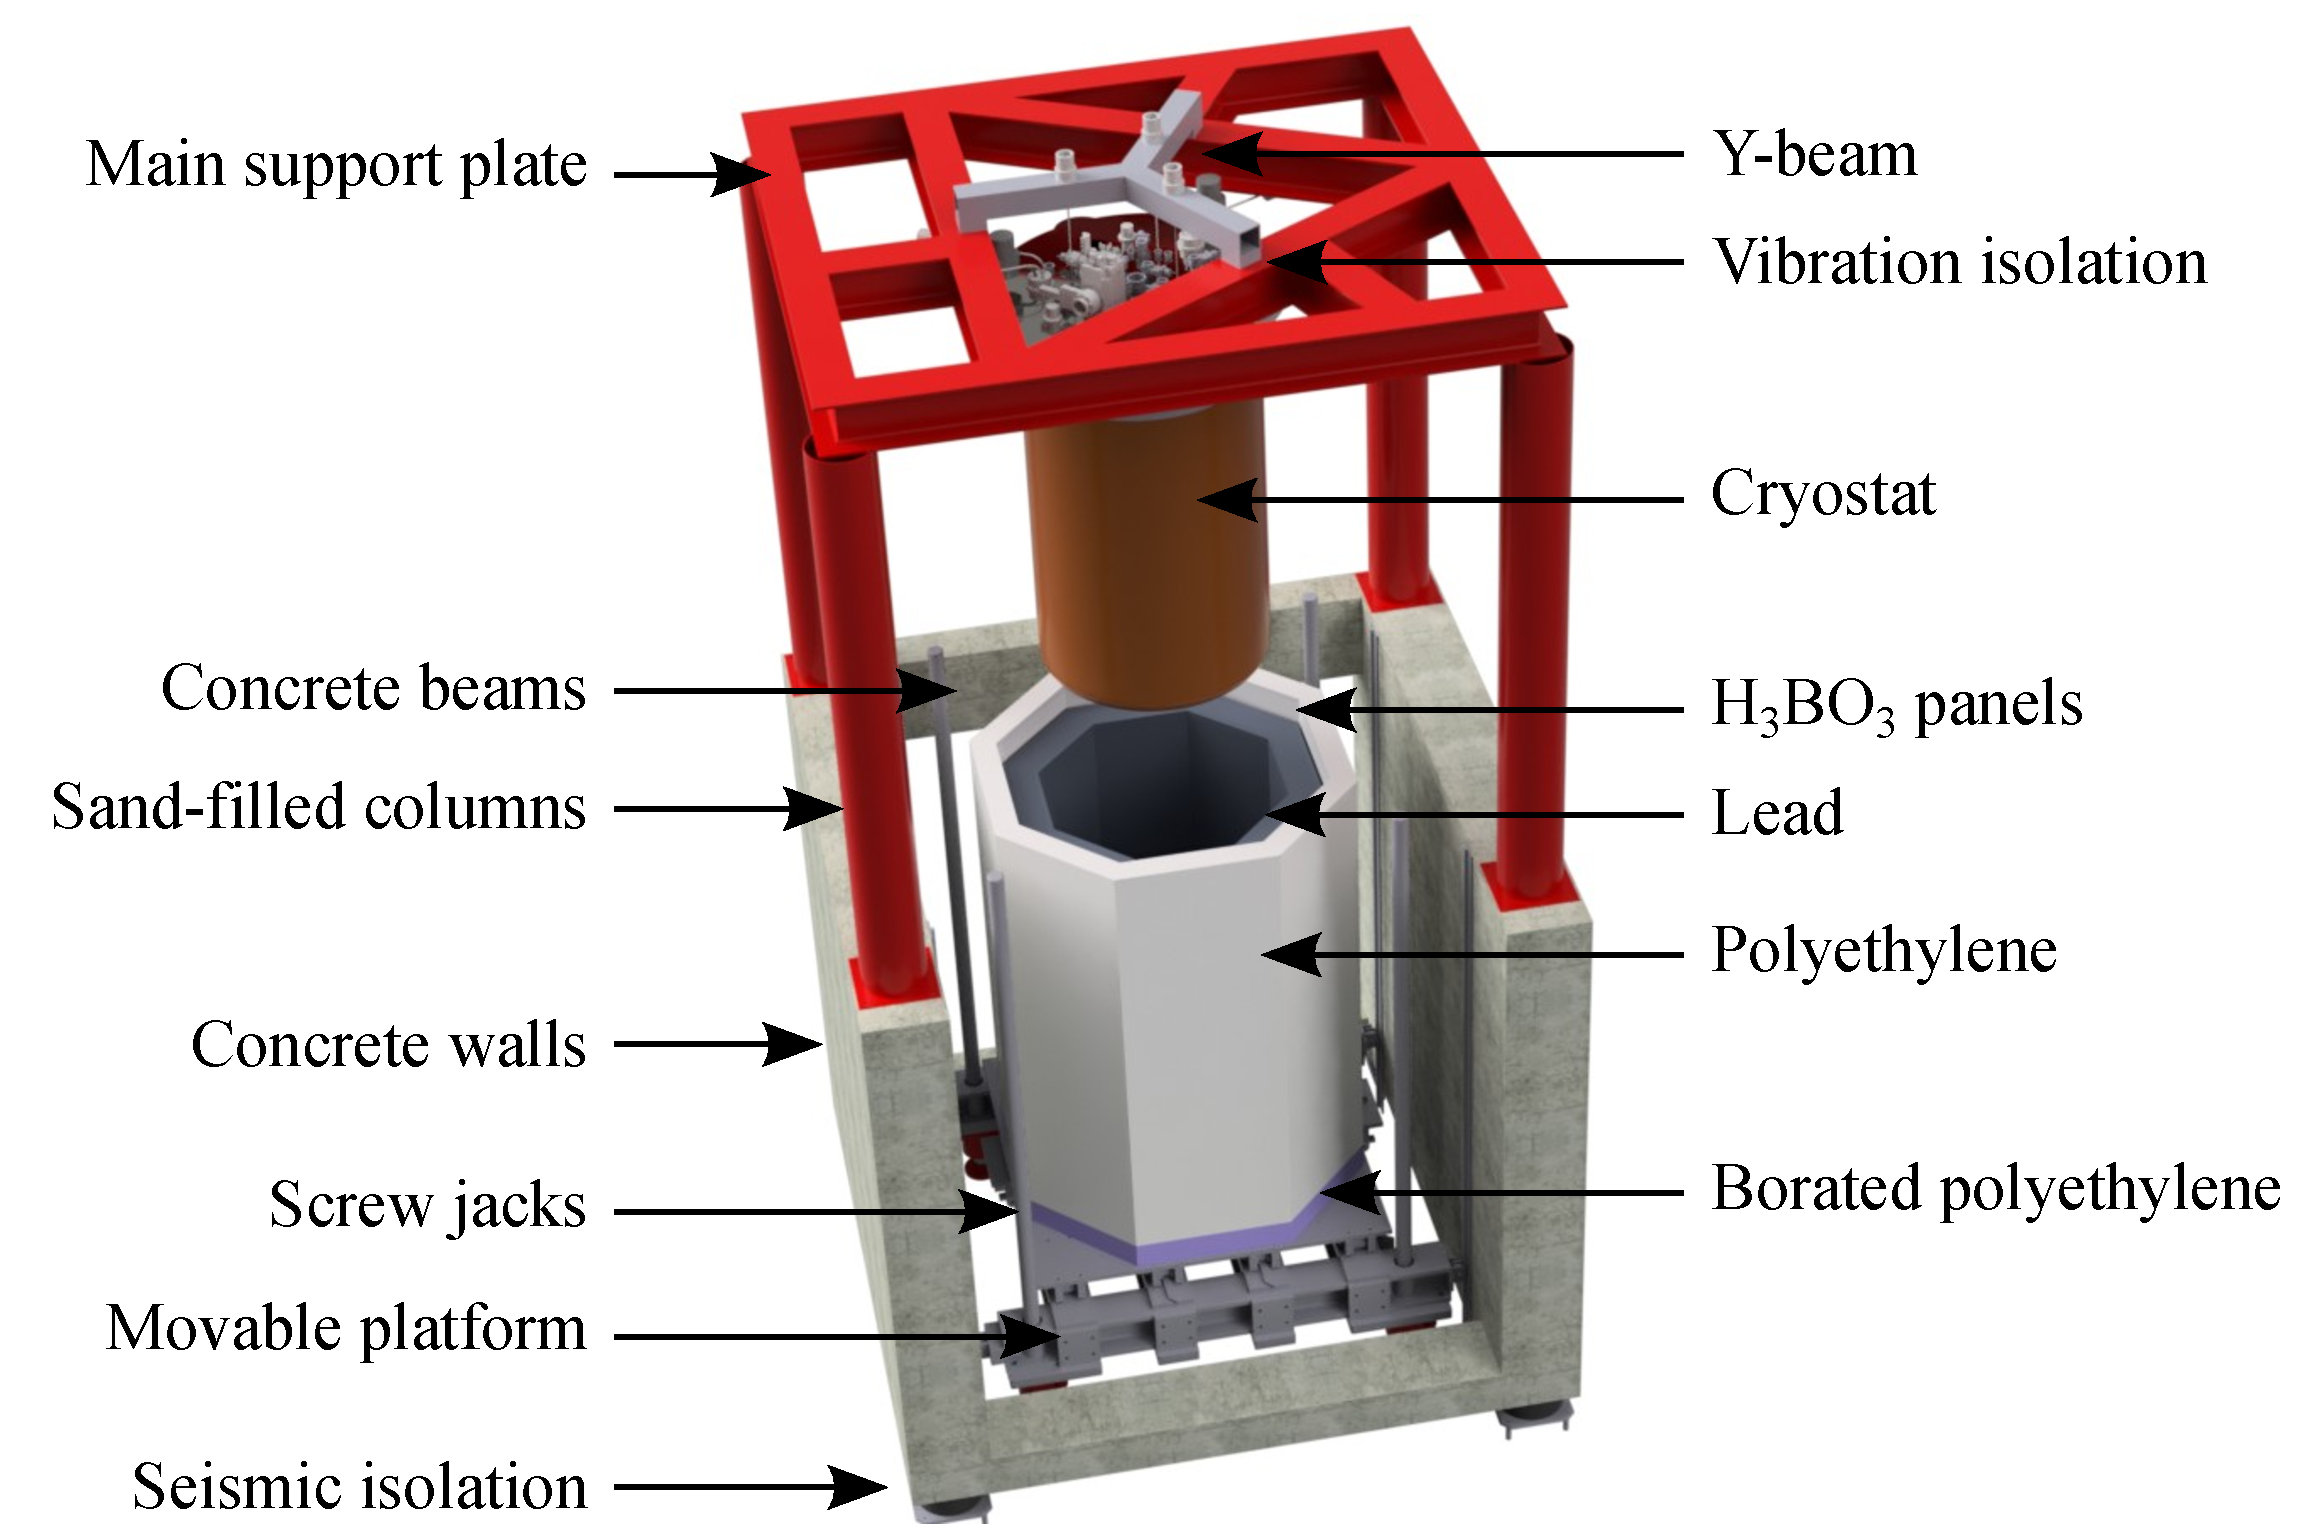
\includegraphics[width=\linewidth]{Figures/Hut_ShieldingDown_02.pdf}
    \caption[The external shielding and supports of the CUORE cryostat.]
    {The external shielding and supports of the CUORE cryostat.
    The external lead shields, with polyethylene and borated polyethlyene, is shown lowered down below the cryostat and is raised up around the cryostat during operation.
    The crystat is suspended above, and the support structure is designed to minimize the mechanical coupling of the cryostat to the outside world and the resultant vibrational noise.}
    \label{fig:external_shielding}
\end{figure}
Inside the 4-K stage of the cryostat, additional 6 cm thick lead shielding is used to further reduce radioactive backgrounds. This shielding comprises over 4 tonnes of ancient shipwrecked lead \cite{roman_lead} and covers the sides and bottom of the cryostat.
As lead when extracted from the ground contains $^{210}$Pb from the $^{238}U$ decay chain with a half-life of 22 years, we use this lead that was shipwrecked between 80 and 50 B.C.E. to line this inner shield of our detectors, shown in \autoref{fig:roman_lead_shield}.
This lead has a contamination of $^{210}$Po less than 10 mBq/kg\footnote{$^{210}$Po in modern lead can reach values of 2500 Bq/kg.} and is thus more suitable for use in the most sensitive regions of our cryostat \cite{ALESSANDRELLO1998163}.  
\begin{figure}
    \centering
    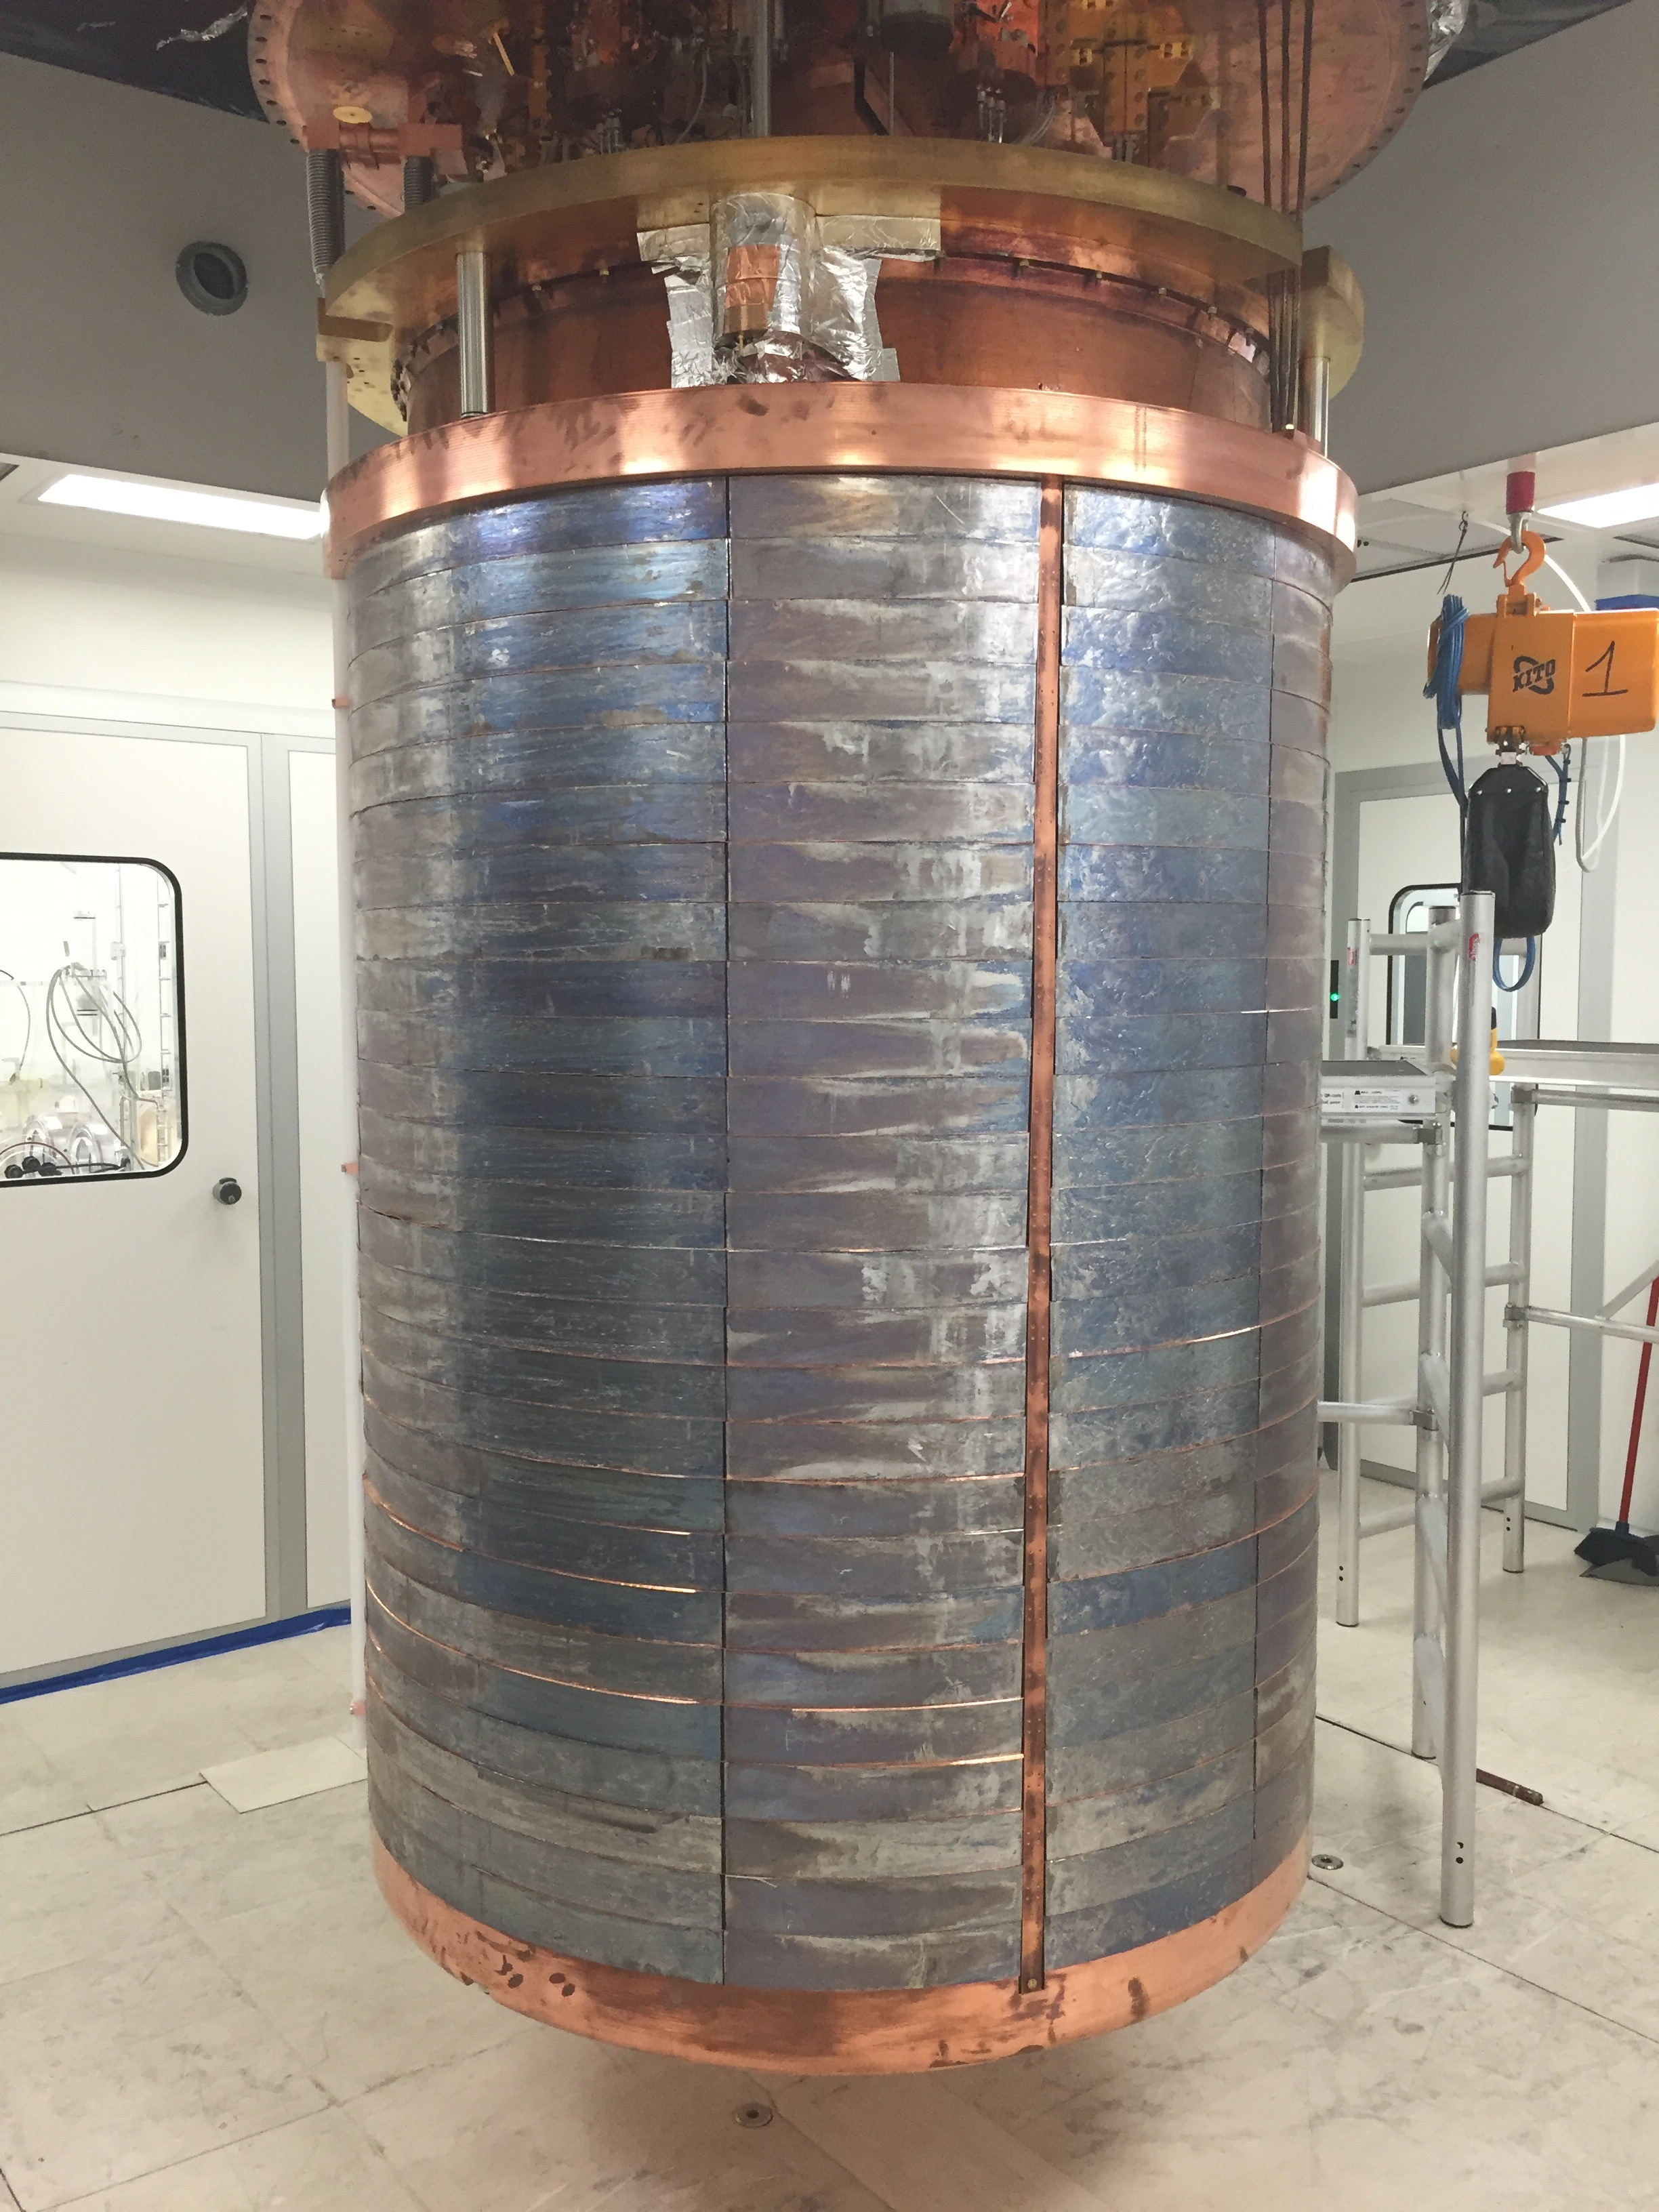
\includegraphics[width=0.4\linewidth, height=0.4\pageheight, keepaspectratio]{Figures/roman_lead_shield.jpg}
    \caption[The roman lead shield installed inside the 4-K vessel.]
    {The roman lead shield installed inside the 4-K vessel. The shield extends laterally around the detector region and a separate piece is below (not visible).}
    \label{fig:roman_lead_shield}
\end{figure}
The 600-mK plate holds the 50-mK plate, which in turn holds up the 10-mK plate, with a double Kevlar rope and a copper rod, respectively.
This rope is used to minimize the heat load at these coldest stages with the least cooling power, see \autoref{tab:cryostat_cooling_power}, and the copper rod is used due to background constraints near the detector region.
Below the 10-mK plate but thermally connected with the 50-mK stage, there is an additional lead shield, consisting of 2 tonnes of modern lead in five 6 cm disks between two copper plates, above the detectors.
This is the final main shield for gammas produced in components of the cryostat, although the copper plate that holds the crystals, called the tower support plate (TSP) also shields the detectors which are mounted to the bottom of the plate.
The TSP hangs separately from the rest of the cryostat and is suspended from the steel Y-beam on three Minus K\footnote{\RaggedRight\url{https://www.minusk.com/}} vibration isolators on the MSP.
Part of the suspension is Kevlar rope that connects the TSP to the copper and steel suspension rods above, which, in addition to reducing the thermal load of the detector array, also serves to protect the crystals in case of a seismic event. 
This assembly acts to cause the detectors to essentially hang freely and avoids pendulum-like low frequency oscillations of the tower array which would cause frictive heating.
While the 50-mK plate and vessel are composed of OFC copper like the warmer stages, the 10-mK plate and vessel, the copper holding the top lead, and the TSP are all comprised of NOSV copper due to the strict background requirements of parts in the detector region.
In addition, the side of the 10-mK plate facing the detector is covered by thin NOSV copper tiles that had been cleaned with the same procedure as for copper in the tower frames.
    
\subsubsection*{Cryostat Cooling Systems}
\label{sssec:Cooling Systems}
Not only does the cryostat shield the detectors from radiation, but it also needs to cool the detectors to temperatures of $\sim$10 mK.
Therefore, a custom dilution refrigerator built by Leiden Cryogenics\footnote{\RaggedRight\url{http://www.tokyoinst.co.jp/product_file/file/LCG01_cat01_ja.pdf}} is used as the main cooling mechanism of the cryostat.
A dilution refrigerator works by taking advantage of the phase boundary between dilute and concentrated phases of a $^3$He and $^4$He mixture, shown in \autoref{fig:He_phase_diagram}.
In the mixing chamber of the dilution refrigerator on the 10~mK stage of the CUORE cryostat, $^3$He flows from the concentrated phase to the dilute phase.
This process extracts energy from the environment of the mixing chamber, and, by extension, the coldest stages of the cryostat, as energy is required to move the $^3$He across the phase boundary\footnote{Of course, the Universe's entropy is not reduced by this exchange and additional energy is used to induce this endothermic cooling.}.
As noted in \autoref{ssec:CUORE-0}, one of the main cryostat changes between the previous experiments of CUORE-0 and CUORE was the change to a cryogen-free cryostat that uses pulse tubes instead of an external supply of liquid nitrogen, helium, and a 1~K bath.
This change allows for increased livetime of the experiment as data-taking does not need to be interrupted by the need to refill the bath, especially as this would become even more disruptive given the tonnes of material that would need to be cooled.
However, this does come at a cost of increased mechanical noise as the five pulse tubes in CUORE input mechanical vibrations onto the cryostat.
Worsening this issue, the five pulse tubes\footnote{PT415-RM from Cryomech \url{https://www.cryomech.com/products/pt415/}} on CUORE are not symmetrically aligned due to space constraints, and it is nontrivial to find a phase configuration that minimizes the noise, requiring an in-depth scan of varying pulse tube phases to determine when the mechanical noise induced by the pulse tubes is minimized over the detectors.

\begin{figure}[htbp]
    \centering
    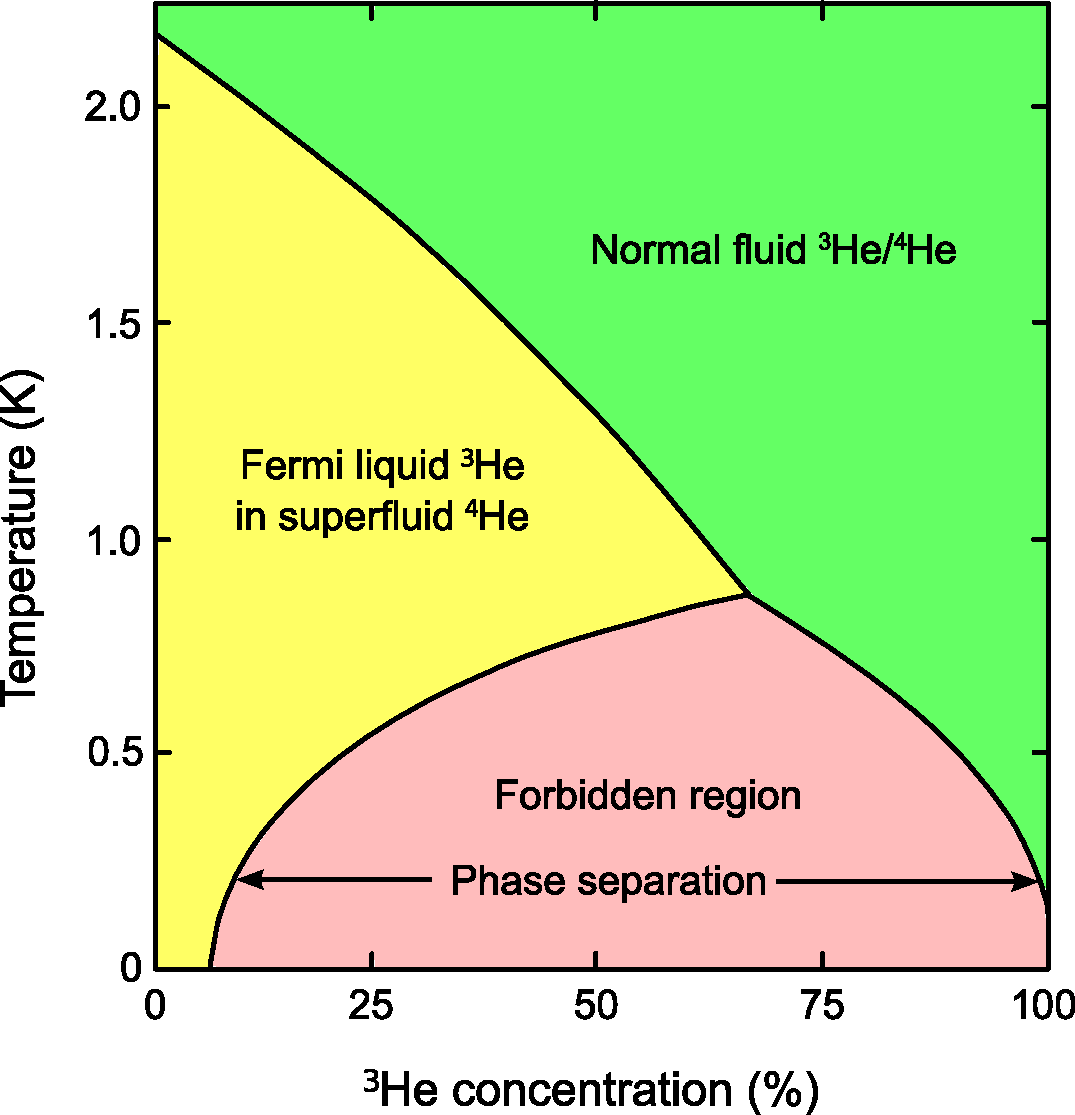
\includegraphics[width=0.6\linewidth]{Figures/Helium_phase_diagram.pdf}
    \caption[Phase diagram for $^{3}$He and superfluid $^{4}$He.]
    {Phase diagram for $^{3}$He and superfluid $^{4}$He.
    The separation between the dilute and concentrated phases provides the power that cools the cryostat down to mK-scale temperatures.}
    \label{fig:He_phase_diagram}
\end{figure}

Inside the cryostat, the components necessary for the operation of the dilution refrigerator are the mixing chamber on the 10-mK plate, the heat exchanger on the 50-mK plate, and the still on the 600-mK plate.
Outside the cryostat, the pulse tubes are responsible for pumping the $^3$He out of the still and back down into the mixing chamber.

In addition to the dilution refrigerator and pulse tubes, an additional system called the Fast Cooling System is also used to cool down the CUORE cryostat from room temperature.
This system is needed since pulse tubes are not designed for sustained operations at warm temperatures and the tonnes of material that is needed to be cooled down.
With the Fast Cooling System, a helium exchange gas is pumped into the IVC at a pressure of $\sim1$bar, which cools the cryostat down to 200 K.
Once this occurs, the pulse tubes are turned on, and later, once the cryostat reaches 50 K, the Fast Cooling System is turned off and and nearly all of the exchange gas is removed, with only a few mbar left to assist with the cooldown of the coldest stages down to 10 K.
The cooldown is finally completed by the DU, which cools the detectors down to 10 mK.
With these systems, the cooldown of the CUORE cryostat can be effected in $\sim20$ days.

\begin{table}[htbp]
    \centering
    \begin{tabular}{c|c}
    \hline
    \hline
    Thermal Stage     & Cooling Power \\
    \hline
    40-K     & 40~W \\
    4-K      & 1.5~W \\
    Dilution unit &  2 mW at 100~mK \\
    Dilution unit*    & 10~$\mu$W at 12~mK \\
    \hline
    \hline
    \end{tabular}
    \caption[The cooling power of the cryostat at varying thermal stages.]
    {The cooling power of the cryostat at varying thermal stages.
    The power is maximized in warmer stages, but decreases significantly towards the coldest stages.
    The values here come from the manufacturers of the pulse tubes and Dilution unit, except for the thermal power of the dilution unit at 12 mK which was determined in a test cryostat (*).}
    \label{tab:cryostat_cooling_power}
\end{table}
\subsubsection*{Cryostat Radiopurity}
\label{ssec:Cryostat_Radiopurity}
As mentioned above, the cryostat also needs to both shield the detectors from outside radioactive sources and simultaneously not contribute to the radioactive backgrounds in the detectors.
It is for this reason, for example that high-purity NOSV copper is chosen for the cryostat components closest to the detectors and that the 4.5 tons of side and bottom lead shielding was chosen to be low-radioactivity ancient Roman lead.
In addition, in order to minimize the effect of cosmogenic activation on the background, the entire CUORE cryostat was assembled and stored underground, although the process of machining and cleaning the components needed to be undertaken aboveground.
The background contamination of these ``far" components, as opposed to the ``near" components in \autoref{tab:NearDetectorSources_Bulk}, is shown in \autoref{tab:FarDetectorSources_Bulk}. 

\begin{table}[htbp]
\centering
\caption[90\% upper limits of $^{232}$Th and $^{238}$U bulk contamination of sources in the cryostat and external shielding.]
{90\% upper limits of $^{232}$Th and $^{238}$U bulk contamination of sources in the cryostat and external shielding.
Table from \cite{Alduino:2017qet}.}
\label{tab:FarDetectorSources_Bulk}
\begin{tabular}{lll}
\hline
\hline
Material         & $^{232}$Th [Bq/kg]         & $^{238}$U [Bq/kg]    \\
\hline
Cu OFE             & $<6.4\times10^{-5}$ & $<5.4\times10^{-4}$      \\
Roman Pb            & $<4.5\times10^{-5}$ & $<4.6\times10^{-5}$      \\
Modern Pb            & $<1.4\times10^{-4}$ & $<1.4\times10^{-4}$      \\
Super-insulation  & $(11\pm2)\times10^{-3}$ & $<2.4\times10^{-3}$      \\
Rods  & $(4\pm2)\times10^{-4}$ & $(8\pm2)\times10^{-4}$      \\
300-K Plate & $(4.5\pm0.5)\times10^{-3}$ & $(1.6\pm0.5)\times10^{-3}$      \\
\hline
\hline
\end{tabular}
\end{table}

As shown in \autoref{eq:sensitivity_short}, the sensitivity of CUORE to \zeronubb~depends on the inverse square root of the background near the decay Q-value.
As such, the background goal of CUORE is to have no greater than 0.01 counts/keV/kg/yr in the region of interest (ROI) defined to be a 100 keV interval from 2470 keV to 2570 keV.
The simulated effect of all the sources, including from cryostat components and shielding, is shown in \autoref{fig:cuore_background_budget}.

\begin{figure}[htbp]
\centering
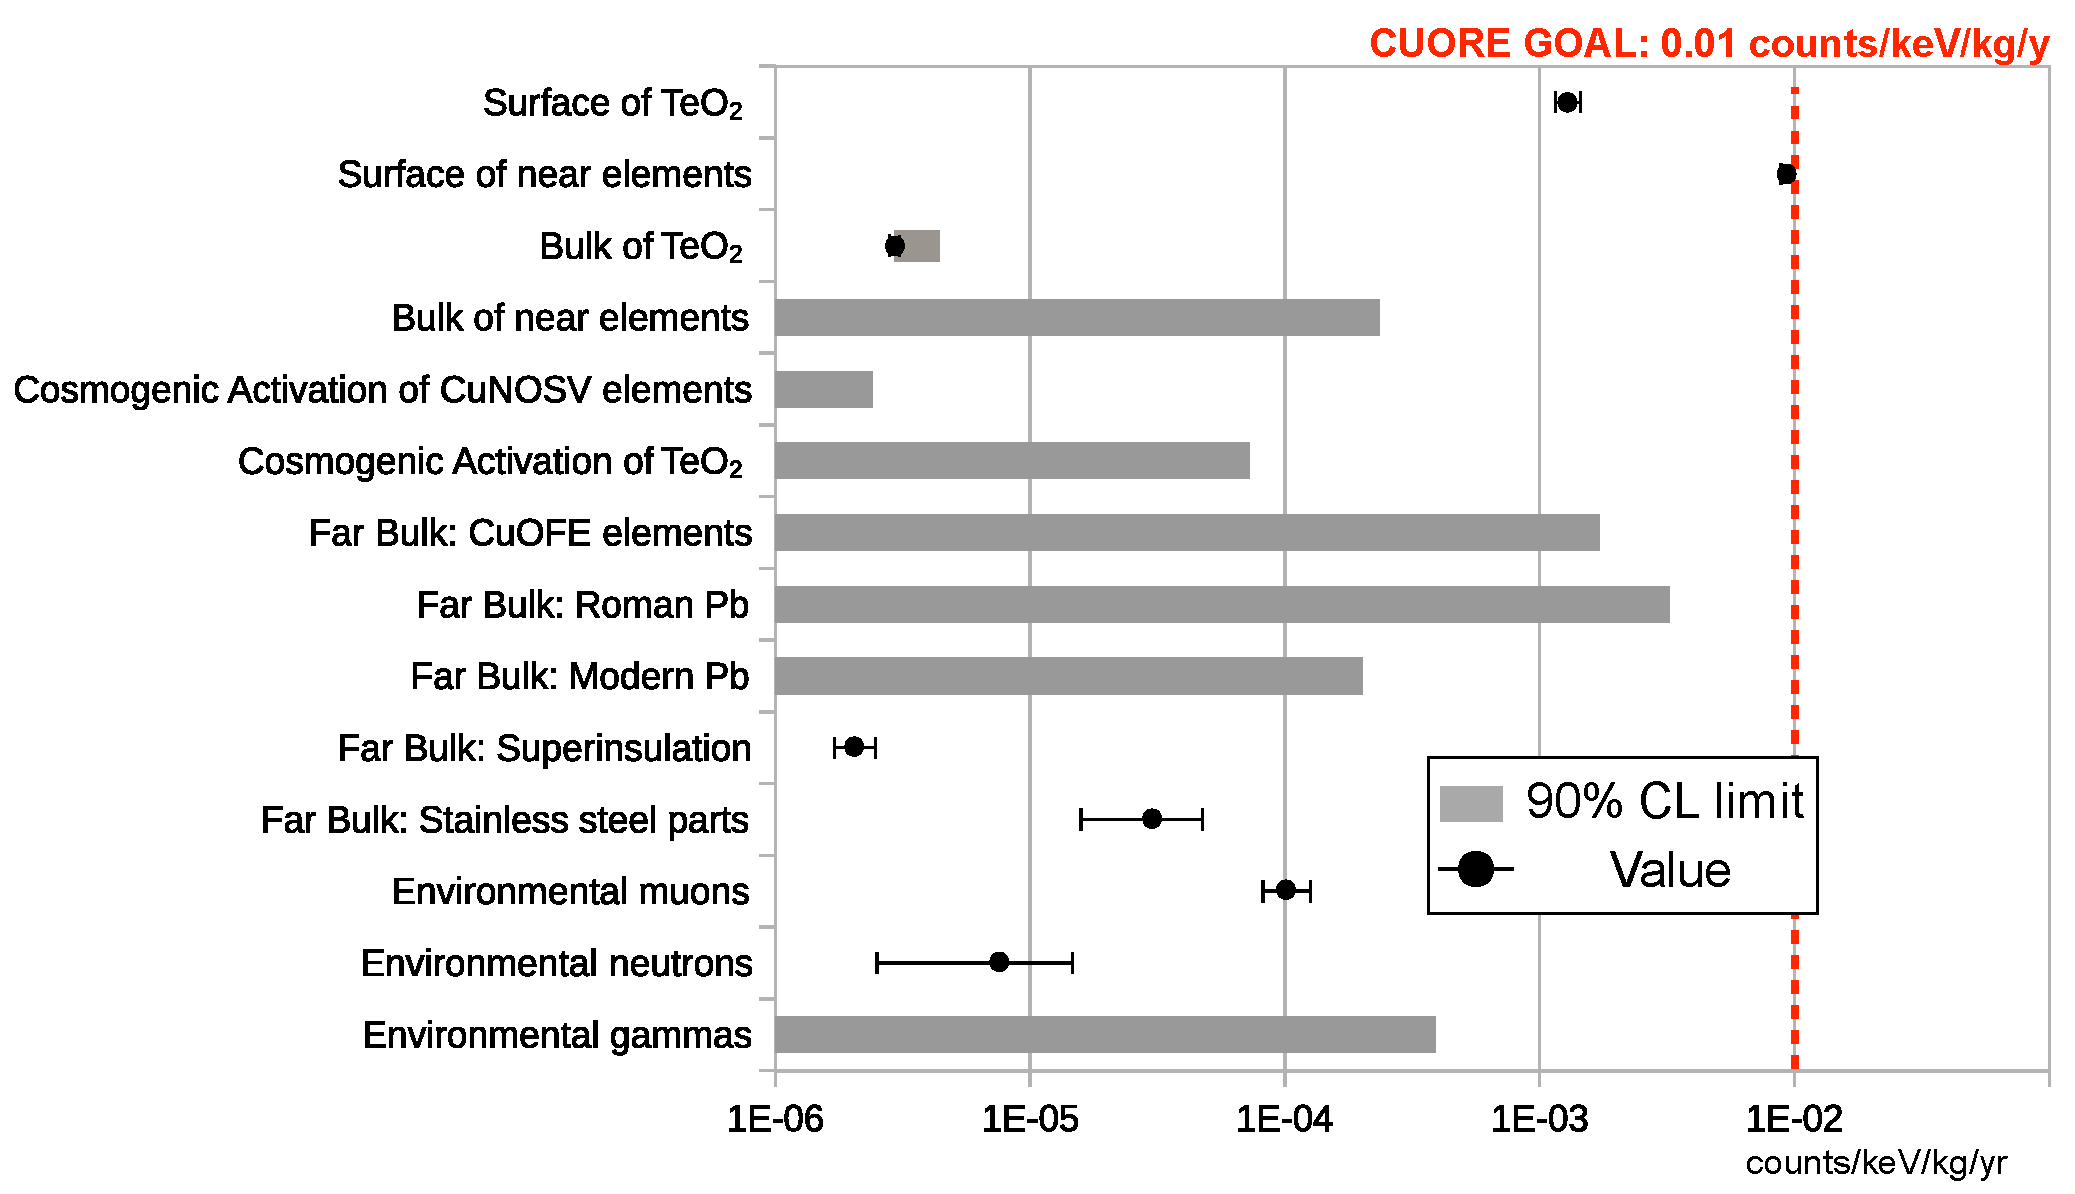
\includegraphics[width=0.8\linewidth]{Figures/CUORE_background_budget}
\caption[CUORE background budget.]
{CUORE background budget.
The CUORE goal is 0.01 counts/keV/kg/y with most of the background due to the surfaces of cryostat elements nearest to the crystal and the bulk of the Roman lead.}
\label{fig:cuore_background_budget}
\end{figure}
\chapter{Detector Calibration System}
\label{chap:DCS}

As described in \autoref{ssec:Particle Detectrion with Bolometers} and shown in \autoref{fig:Sample_pulse}, the actual values that CUORE detects are the changes in resistance of the NTDs as the crystals change temperature due to particles depositing energy.
However, this energy response is strongly non-linear and needs to be calibrated along a range of energies.
Therefore, in order to calibrate these NTD responses to energy depositions in the crystals, and considering the 5 keV energy resolution goal for CUORE, the Detector Calibration System (DCS) was developed.
This system enables the experiment to independently characterize the thermal response over a range of energies up to and beyond the Q-value of \zeronubb~for each of the 988 \teotwo~crystals in CUORE.
This is done by occasionally inserting radioactive sources with known intensity and composition, viz. $^{232}$Th, that emit mono-energetic particles such as photons that will deposit energy into the detectors.
The thermal response of the detectors can then be mapped one-to-one with these known energies, and thus the entire detector array can then be individually calibrated. The hardware and simulation for this work in described in this chapter, and a discussion of how the software analyzes calibrations is described in \autoref{ssec:Calibration}.

\section{Overview}

Making such a system as the DCS, that can meet this goal in the CUORE cryostat is an enormous technical challenge.
As noted in \autoref{sec:Predecessor Experiments} and shown in \autoref{fig:CUORE-0_cryostat_schematic}, calibration sources in CUORE-0 and Cuoricino could be deployed by hand inside the innermost lead shielding to irradiate a single tower of detectors.
However, with 19 towers of crystals making up the CUORE detector array, and with thicker layers of shielding, efficiently deploying sources inside the cryostat requires the sources to be placed in between the towers and inside the roman lead shielding.
This significantly adds to the challenge of such a system as the calibration sources need to be both inserted and retracted from the coldest region of the cryostat on a regular basis.
The main challenges can be summarized as follows: 
\begin{itemize}
\item Calibrate all 988 crystals in as short a time as possible
\item Minimize thermal disturbance to the crystat and the crystals
\item Negligibly contribute to the background in operation
\end{itemize}

The solution to these issues was the Detector Calibration System developed at Wisconsin and at Yale.
With this system, shown in \autoref{fig:DCSintegration}, 12 Kevlar strings containing copper capsules with 2\% thoriated tungsten wire are inserted into the cryostat from above the 300-K stage down into the detector region at the 10-mK and 50-mK stages. 

\begin{figure}[htbp]
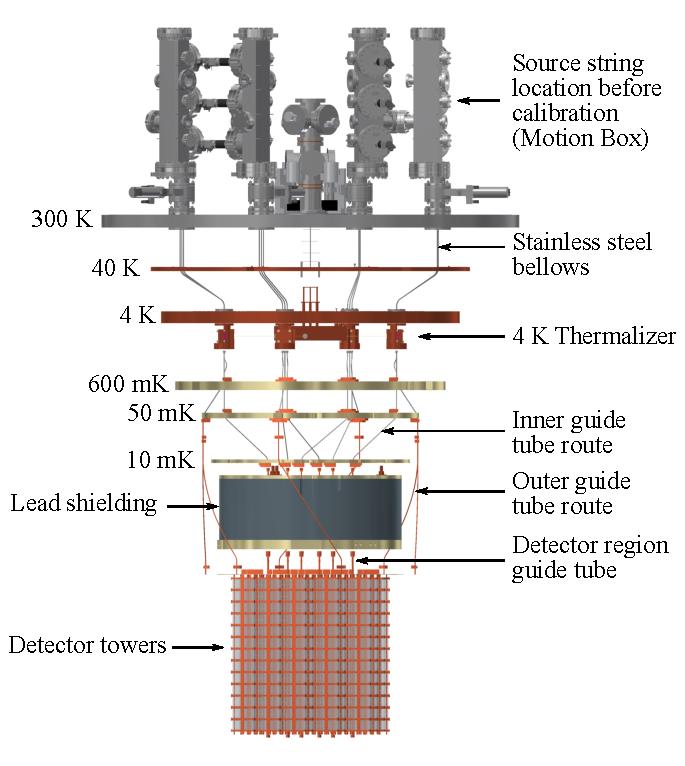
\includegraphics[width=\linewidth]{Figures/DCSintegration.pdf}
\caption[The CUORE Detector Calibration System (DCS).]
{The CUORE Detector Calibration System (DCS).
12 kevlar strings are deployed intermittently into the cryostat through individual tubes through the stages of the cryostat.
6 of the strings are deployed through the inner guide tubes into the 10 mK region of the cryostat between the detector towers, and the other 6 strings are deployed outside the towers in the 50 mK region.
Figure from \cite{Cushman:2016cnv}.}
\label{fig:DCSintegration}
\end{figure}

\section{Calibration Hardware}

The DCS can be divided into a few separate hardware components: the 12 source strings, the 12 sets of guide tubes for the string in the cryostat, the 4 motion boxes, the 4-K thermalization system, and the cabling for the software control system.
Each of these sets of components has different technical challenges, particularly for the calibration tubes nearest to the detectors that have stringent radioactivity requirements, and are described in more detail in this section.

\subsection*{Calibration Source Strings}
There are 12 calibration source strings that are deployed in to the detector region in order to calibrate the 19 towers of CUORE.
These source strings consist of copper capsules covered in PTFE heat shrink tubing that enclose the 2\% thoriated tungsten source inside, shown in \autoref{fig:source_carrierA}.
The copper is crimped on top and bottom in order to hold it onto the Kevlar string and to hold the source inside, and the Teflon heat shrink reduces the friction between the copper capsules and the DCS guide tubes. In addition, the bottom 8 capsules have reducing spacing and are wider than the other capsules, shown in \autoref{fig:source_carrierB}.
As the sources are deployed into the cryostat under their own weight, these heavier capsules (called ``weight" capsules, opposed to the other ``source" capsules\footnote{Despite the naming convention, all the copper capsules contain radioactive sources.}), and particularly the PTFE guide ball, assist the strings with lowering into the funnels between stages and in detecting obstructed paths.
For example, if the tubes are not perfectly vertically centered, the guide ball will be caught by the funnel and guide the string down into the funnel, where the weight of the capsules will pull the string down into the funnel correctly.
This is opposed to a case where, if there were no weight capsules, some string would fall into the tube, but the rest would drape off the side of the funnel and fail to deploy since the string would not be sufficiently pulled down into the tube.

\begin{figure}[htpb]
\begin{center}
\begin{subfigure}[b]{0.60\textwidth}
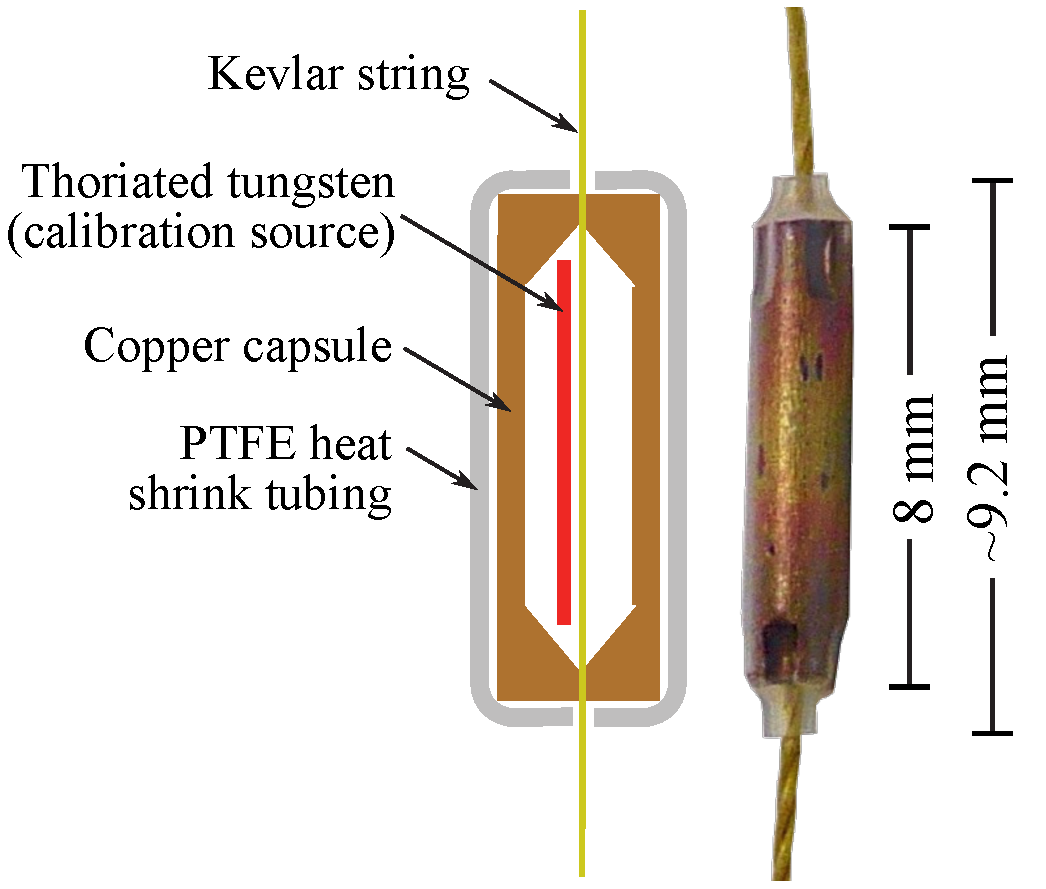
\includegraphics[height=2.2in]{Figures/source_capsule_schematic.pdf}
\caption{}
\label{fig:source_carrierA}
\end{subfigure}
\begin{subfigure}[b]{0.15\textwidth}
\includegraphics[height=2.7in]{Figures/string_bottom.pdf}
\caption{}
\label{fig:source_carrierB}
\end{subfigure}
\end{center}
\caption[(a) Schematic and photograph of an assembled source capsule. (b) Photograph of five heavier bottom capsules and PTFE ball at the bottom of a source string.]{(a) Schematic and photograph of an assembled source capsule. (b) Photograph of five heavier bottom capsules and PTFE ball at the bottom of a source string.}
\label{fig:source_carrier}
\end{figure}
 
Recalling that one of the design goals for the DCS is to calibrate all 988 crystals in as short a time as possible, the strings are configured, when fully deployed in the cryostat, to optimize coverage on all the crystals, as the time it takes to calibrate the detector array is limited by the time it takes the least-irradiated crystals to calibrate.
To this end, the calibration sources are configured in a double-hexagonal pattern, as shown in \autoref{fig:Calibration_source_top_view} with the inner source strings inside the 10-mK vessel irradiating the towers and floors closest to the center and the outer strings outside the 50-mK vessel irradiating the towers and floors furthest from the center.
The inner calibration strings are located about 2 cm from the faces of the crystals, and the outer calibration strings are about 18 cm away from the crystals, although they are shielded from the crystals by the 10-mK and 50-mK vessel.
As a result of this geometry, there are two main differences between the copper capsules in each calibration string and between the inner and outer strings, viz., the bottom and top capsules of each string have a boosted activity relative to the capsules in the middle of the string, and the capsules in the outer strings have a boosted activity relative to their counterparts in the inner strings, with the specific activities of each described in \autoref{tab:calibration_activities}
In addition, there is one more capsule on the inner strings relative to the outer strings, which is due to the fact that when the strings were made, the activities were lower than anticipated and needed a more significant boost at the top of the calibration string.
The reason for this asymmetry for the activity of the capsules on each string is to have roughly equal rates on each crystal on each floor, and, since the calibration strings are only slightly longer than the towers themselves\footnote{The inner and outer calibration strings have an active region 80 and 83 cm long, respectively.}, these edge effects need to be considered for optimal calibration.
The spacing of the source capsules is designed such that each floor sees roughly 2-3 adjacent capsules at a time, and the vertical geometry of the strings in their nominal vertical positions is shown in \autoref{fig:Calibration_source_tower}.

\begin{figure}[htpb]
\begin{center}
\begin{subfigure}[b]{0.5\textwidth}
    \includegraphics[height=3.25 in]{Figures/CUORE_calibration_location.pdf}
    \caption{}
    \label{fig:Calibration_source_top_view}
\end{subfigure}
\begin{subfigure}[b]{0.40\textwidth}
\includegraphics[height = 3.5 in]{Figures/Cuore_tower_calibration.pdf}
\caption{}
\label{fig:Calibration_source_tower}
\end{subfigure}
\end{center}
\caption[(a) A top-down schematic of the calibration source strings in the cryostat.
(b) A side-view schematic of an inner and outer calibration string next to a tower.]
    {(a) A top-down schematic of the calibration source strings in the cryostat.
    The inner strings irradiate the innermost towers, and the outer strings irradiate the outermost towers.
    Due to space constraints, the outer sources are located outside the 50-mK vessel.
    (b) A side-view schematic (horizontal axis not to scale) of a tower with an adjacent inner (right) and outer (left)  calibration string.
    Figures adapted from \cite{Cushman:2016cnv}.}
\label{fig:Calibration_source_locations}
\end{figure}

\begin{table}[htbp]
    \centering
    \caption[The number of capsules and activities of each calibration source.]
    {The number of capsules and activities of each calibration source.
    The capsules are listed from bottom to top, with the 8 capsules corresponding to the weight capsules on the string.
    For the activity, the activity of each capsule is listed, along with the total summed activity of that component.
    In total, the activity of the inner strings is 3.6 Bq, and the activity of the outer strings is 19.4 Bq, with the activities listed as the activity of the $^{208}$Tl decay in the $^{232}$Th decay chain.}
    \label{tab:calibration_activities}
    \begin{tabular}{lccc}
    \hline 
    \hline
        String type & Capsules & Activity (Bq) & Summed Activity (Bq) \\
        \hline 
        \multirow{3}{*}{Outer} & 8 & 0.64 & 5.12 \\
        & 20 & 0.48 & 9.52 \\
        & 5 & 0.95 & 4.75 \\
        \hline
        \multirow{4}{*}{Inner} & 8 & 0.07 & 0.54 \\
        & 21 & 0.09 & 1.95 \\
        & 4 & 0.08 & 0.31 \\
        & 1 & 0.80 & 0.80 \\
        \hline
        \hline
    \end{tabular}
\end{table}

\subsection*{Motion Boxes}
On top of the cryostat, there are four motion boxes, shown in \autoref{fig:motion_box}, that contain the DCS calibration strings while they are not being deployed and the motors that control the motion of the strings.
The motion boxes have dimensions $12.6\times7.9\times60.7~\textrm{cm}^3$ constituting a 6 L volume.
There are three strings in each motion box that are wound up on each of the calibration string spools internally.
These calibration strings can then be deployed independently and simultaneously down through three guide tubes in the motion box down into the cryostat.
Inside the motion boxes, each acts as an independent vacuum system during, only connecting to the IVC when calibration strings are being deployed into the cryostat.
A proximity sensor at the bottom of the motion box detects when the copper capsules enter and disturb the electromagnetic field produced by the sensor.
This allows for us to determine when individual source capsules or the weight capsules\footnote{The sensor is unable to resolve the denser-packed weight capsules and triggers continuously while they are in the sensor.} move either into or out of the motion box.
\begin{figure}[htpb]
\includegraphics[width=0.9\linewidth]{Figures/motion_box.pdf}
\caption[A rendering of a single motion box from two different angles.]{A rendering of a single motion box from two different angles. The motion box is mounted vertically with the PEEK flange on top of the cryostat with the three source strings spools above. The windows on each motion box allow for the source strings to be observed from outside.}
\label{fig:motion_box}
\end{figure}
The motion box has 3 CF
The motion boxes contain all of the electronic controls that enable and monitor the deployment of the calibration strings into the crystat.

\subsection{Guide Tubes}


\begin{figure}[htbp]
    \centering
    \includegraphics[height=0.4\paperheight]{Figures/thermal_coupling.pdf}
    \caption[A diagram showing the thermal couplings of the DCS tubes for both the internal and external sources.]
    {A diagram showing the thermal couplings of the DCS tubes for both the internal and external sources.
    In order to minimize the thermal load on the cryostat, there are multiple breaks in the DCS tubes with funnels for the calibration sources to pass through.
    Near the detectors, the tubes switch from being stainless steel with low thermal conductivity to low-background copper.
    For the external tubes, there are no tubes below the lead shield and the source capsules hang freely.
    Figure from \cite{Cushman:2016cnv}.}
    \label{fig:dcs_thermal_coupling}
\end{figure}


\subsection{Thermalization and Thermometry}
In order to deploy 12 calibration source strings from 300 K down to 50 or 10 mK, the sources need to be cooled as much as possible before they reach each stage of the cryostat or even the black-body radiation from the sources will cause the temperature of the crystals and the cryostat to rise excessively and possibly dangerously. Most of the mass, and therefore the heat \color{red} find a better word than heat \color{black} is carried in the copper capsules. The kevlar that holds the capsules is a poor conductor of heat \color{red} Citation Needed \color{black} compared with the capsules, which is a necessary feature, in addition to its strength, as the kevlar will form 12 continuous lines from the motion boxes at 300 K down to the detector region at 10 mK.

To effect this cooling on the source strings, multiple methods are used. The main cooling mechanism used is from the copper thermalizers located at the 4 K plate, shown in \autoref{fig:DCS_4K_schematic}. These thermalizers consist of a moving copper block and a copper base, with the copper block pushed away by a spring. The copper block is activated by another kevlar string that, when pulled, pushes the copper block onto the copper base. The cooling time decreases as the force between the copper block and capsule increases, and a force of 32 N was chosen This cooling is performed at the 4K stage as the cryostat has the most cooling power at this stage \color{red} Link to the cooling power table \color{black}. Most of the cooling of the capsules is done at this position and this thermalization process over an entire string is a significant fraction of its total deployment time.


\color{red}connect these figures \color{black}
\begin{figure}[htbp]
    \centering
    \includegraphics[width=0.8\linewidth]{Figures/thermalization_system_labeled.pdf}
    \caption[A cutaway drawing of the 4-K thermalization system on CUORE.]
    {A cutaway drawing of the 4-K thermalization system on CUORE.
    When the linear actuator is fully down, the hanging mass hangs freely from the rotary feedthrough, which is then connected through a pulley to the copper block.
    This applies the 32 N of force acting on a capsule in order to cool it down to 4 K.}
    \label{fig:DCS_4K_thermalizer}
\end{figure}

\begin{figure}[htbp]
    \centering
    \includegraphics[width=0.8\linewidth]{Figures/Thermalizer_schematic_labeled.pdf}
    \caption{Caption}
    \label{fig:DCS_4K_schematic}
\end{figure}


Another way in that heat is removed from the source strings is due to the contact with the walls of the guide tubes. This cooling, however, is limited in two main ways: by the angle of the tube as steeper angles provide less contact with the source capsule and by the heat capacity and thermal contact of the tube with each stage as some tubes, namely those at 600 mK will warm up to 4K or beyond. Below the thermalizers, the inner strings also go through a ``chicane" \color{red} Should I put this in quotes? Also, add reference to figure\color{black} which increases the contact between the capsules and the tubes. This is done to further increase the rate at which heat is removed from the capsules as the cooling on these sources that are to be deployed at the 10 mK stage are the most critical to cool, but the cooling power decreases at colder stages. 

\begin{figure}[htbp]
    \centering
    \includegraphics[width=0.8\linewidth]{Figures/ChicaneThermometers.JPG}
    \caption[The chicane thermometers.]
    {The Chicane thermometers under the 4K stage.
    These cernox thermometers are used to determine the temperature of the capsules as they leave the 4~K thermalizer into the 600~mK guide tubes.}
    \label{fig:chicane_thermometers}
\end{figure}

\subsection{Software Control of the DCS}
Diagrams to include: pictures of the thermometers, heat loads on the thermometers in different scenarios, 600 mK chicane, 4K thermalizers
\subsection{Impact on Cryostat}

Describe how the calibration affects the state of the cryostat. What are the temperature effects on the plates during the deployment.


\section{Calibration Simulation}
Describe how the simulations for the calibration system are performed. How to determine the best calibration time and effects of pileup.

Figures to include; Geant4 visualization of the sources, rates on the detectors in a calibration, rate dependence on pileup 

\section{Calibration Performance}

Describe how well the calibration system has performed? Also show different strategies for deploying the DCS.

\subsection{Calibration Strategies}

When deploying strings, it would be considerably simpler if one could deploy all the strings simultaneously down into the cryostat; however, there are multiple considerations that need to be taken into account during the operation.
Firstly, one of the main constraints is that no strings can pass through a 4-K thermalizer while it is squeezing on another string.
As the time it takes to squeeze on each set of capsules takes 10-20 minutes, this process takes hours, during which no other string can be moved through the thermalizer.
Secondly, the heat load from the calibration sources themselves is important.
\chapter{Data Acquisition and Processing}

\section{CUORE Data Acquisition}
\subsection{DAQ Electronics Hardware}

\section{Online Data Taking}
\subsection{Signal Triggering}

\section{Offline Data Processing}
\subsection{First-Level Processing}
\subsubsection{Preprocess}
\subsubsection{Amplitude Evaluation}
\subsubsection{Stabilization}
\label{ssec:Stabilization}

The energy dissipated in the silicon heater transfers into the bolometer similarly how a real energy deposition would look in a physics event, and allows for us to understand the response of the detector to fixed-ernergy input across various detector baselines as the temperature of the detectors drifts \cite{ALESSANDRELLO1998454:Si-heater}.

\subsubsection{Calibration}
\label{ssec:Calibration}
\subsection{Second-Level Processing}
\subsubsection{Pulse Shape Analysis}
\subsubsection{Coincidence Analysis}




\chapter{Simulation in CUORE}

This chapter details the simulations used in CUORE

\section{Monte Carlo Method Overview}

\section{Geant4 Simulation Toolkit}

\section{CUORE Reconstruction in Geant4}

\section{Simulating Detector Response}
\chapter{Majoron Decay Search}

\section{Background Sources in CUORE}

\section{JAGS Analysis Software}
\subsection{Markov Chain Monte Carlo}
To perform a search for a spectrum-based rare event, it 
\section{Source Reconstruction}

\section{Majoron Analysis}
When fitting the data with JAGS, the spectrum is split into two main components: the \Mone~spectrum, the \Mtwo~spectrum, and the summed \Msum~spectrum. This is done as the signal events from a Majoron search mostly deposit energy into a single crystal, as is typical of events originating from the bulk of the crystal volume, whereas many other sources that are external to a crystal or on the surface have a much higher probability of depositing energy into more than one crystal. Higher multiplicity spectra are not used, except for identifying the contribution of muons to the background, as they do not add significant information to the fit for other sources. For the fit, each of the possible Majoron spectral indices are considered independently and are shown for each multiplicity in \autoref{fig:SpectralIndicesM1Fit} and \autoref{fig:SpectralIndicesM2Fit}.


\begin{figure}[htbp]
\centering
\begin{subfigure}[t]{0.49\textwidth}
\includegraphics[width=0.9\textwidth]{Figures/Majoron_n1_g4cuore.pdf}
\end{subfigure}
\qquad
\begin{subfigure}[t]{0.49\textwidth}
\includegraphics[width=0.9\textwidth]{Figures/Majoron_n2_g4cuore.pdf}
\end{subfigure}
\qquad
\begin{subfigure}[t]{0.49\linewidth}
\includegraphics[width=0.9\textwidth]{Figures/Majoron_n3_g4cuore.pdf}
\end{subfigure}
\qquad
\begin{subfigure}[t]{0.49\linewidth}
\includegraphics[width=0.9\textwidth]{Figures/Majoron_n7_g4cuore.pdf}
\end{subfigure}
\caption[The fitted contribution of Majoron decays for the different spectral indices in the \Mone~ spectrum.]{The fitted contribution of Majoron decays for the different spectral indices in the \Mone~ spectrum.}
\label{fig:SpectralIndicesM1Fit}
\end{figure}

\begin{figure}[htbp]
\centering
\begin{subfigure}[t]{0.49\textwidth}
\includegraphics[width=0.9\textwidth]{Figures/Majoron_n1_g4cuore_M2.pdf}
\end{subfigure}
\qquad
\begin{subfigure}[t]{0.49\textwidth}
\includegraphics[width=0.9\textwidth]{Figures/Majoron_n2_g4cuore_M2.pdf}
\end{subfigure}
\qquad
\begin{subfigure}[t]{0.49\linewidth}
\includegraphics[width=0.9\textwidth]{Figures/Majoron_n3_g4cuore_M2.pdf}
\end{subfigure}
\qquad
\begin{subfigure}[t]{0.49\linewidth}
\includegraphics[width=0.9\textwidth]{Figures/Majoron_n7_g4cuore_M2.pdf}
\end{subfigure}
\caption[The fitted contribution of Majoron decays for the different spectral indices in the \Mtwo~ spectrum.]{The fitted contribution of Majoron decays for the different spectral indices in the \Mtwo~ spectrum.}
\label{fig:SpectralIndicesM2Fit}
\end{figure}

\chapter{Conclusion}
la la la CUORE still needs more time to discover x...

\section{Future Prospects}
If not, CUPID will solve things.

Insert CUPID lobster plot, maybe a diagram of CUPID or showing a plot for expected alpha backgrounds

\subsection*{Muon Panels}

\backmatter
\bibliographystyle{apsrev4-1}
\bibliography{Bibliography.bib}
\appendix
% Appendices and Bibliography
\chapter{Toy Monte Carlo for Systematics Studies}

Studies of systematics for experiments is generally a difficult process as multiple different effects need to be taken into account.
It is not a trivial problem to determine how uncertainty in one parameter will propagate into a systematic uncertainty on a final result.
For example, an error in the resolution affects how the fit, which is calculated over thousands of channel-dataset pairs, will resolve events near the Q-value.
The only parameter in CUORE that propagates ``easily" is the uncertainty on the efficiency, which affects the result in a simple, linear fashion. However, other parameters, such as the resolution, are, in general, intractable algebraically.
These can be studied directly, however, by performing pseudo-experiments, called Toy Monte Carlo, on generated datasets based on real data that have been perturbed by the uncertainty in a parameter.
For example, to study the effect of uncertainty on the Q-value, pseudo-experiments are performed with a generated signal centered with the Q-value perturbed by the uncertainty (here, 0.5 keV higher and lower) to see how that would have affected the measurement of the signal.


\section{Toy Monte Carlo Overview}

The idea behind pseudo-experiments is a simple one.
If there were a thousand universes each with their own CUORE and taking data for exactly the same amount of time, one would expect to see a thousand different results spread around the ``real" physical result.
However, only one of these results can be observed, so by working backwards, these other results can be replicated to study their features.
For instance, systematic biases such as the bias due to the fit can be straightforwardly studied through the use of these pseudo-experiments.
By scaling up the ``true" signal rate in pseudo-experiments, the fit bias can be directly understood and characterized.

\section{Toy Monte Carlo for \zeronubb}

The generation and fitting procedure for Toy Monte Carlo can be summed up with the following steps:
\begin{enumerate}
\item Fit the real data, $D_0$.
\item Create a model, $H_0$, from the fit to real data.
\item \label{item:generate} From $H_0$, generate new data, $D_i$. Repeat to create as many Toy Monte Carlo as needed. Do not Poisson-float the number of events when determining the p-value.
\item Fit each $D_i$ with the same fitting process as was done to $D_0$.
\item See how parameters from $H_0$ compare with $H_i$
\end{enumerate}

In the case for \autoref{sec:Fit Biases} and \autoref{sec:Systematic Calculations}, this process is slightly different. There, the model needs to be perturbed in some manner when generating the data, so \autoref{item:generate} would then include an alteration of $H_0$ to a new model $H_1$ where the parameter has been perturbed.

Also, the choice of the model to use $H_0$ can be up for some debate. In order to keep the analysis blinded, it is important to finalize the method used beforehand. While for the first PRL paper, we decided to use the fit to data with the signal rate fixed to zero (the null hypothesis) as the base fit to use to calculate all the systematics, it would be better to use the fit to the data with a floating signal rate as the base fit to calculate systematics. Naturally, to evaluate the p-value, one should use the null hypothesis model.


\section{Toy MC Tests}
\subsection*{Goodness-of-fit Tests}
\label{sec:Goodness-of-fit}
One use of Toy MC is to determine how good a particular fit is to the data, particularly at how Poisson fluctuations of the data would affect the fit statistics.
In CUORE, we do this tests with two different methods. One of which is the Kolmogorov-Smirnov (K-S) Test statistic, given by
\begin{eqnarray}
D_n = \sup|F(x) - F_{obs}(x)| 
\end{eqnarray}
where $F_{obs}$ is the cumulative distribution function of the observed data, and $F(x)$ is the cdf of the model in consideration. In this case, it is a cdf of the fit model to the (pseudo)data. An example is shown in \autoref{fig:ksstat}.

The other statistic used to test is the negative log likelihood (NLL) for each of the fits to the ToyMC, shown in \autoref{fig:nll}. This is the (negative) sum of the log likelihoods of the data given a Poisson distribution, namely,
\begin{eqnarray}
L(\lambda; x_1,...,x_n) = -n\lambda - \sum_{j=1}^{n}\ln(x_j!) +\ln(\lambda) \\
-L(\lambda; x_1,...,x_n) = n\lambda + \sum_{j=1}^{n}\ln(x_j!) -\ln(\lambda)
\end{eqnarray}
where lambda is the expected value for the data in a particular bin, $j$, and $x_j$ is the actual data in that bin.
Maximizing the log likelihood (or minimizing the negative log likelihood) is a commonly-used method for fitting, as the log likelihood can be used as an extremum estimator. 
For CUORE, we perform an unbinned fit, which can be thought of intuitively as the limit where all the bins are infinitely small, but the underlying idea is the same.

\begin{figure}
\centering
\includegraphics[width=0.7\linewidth]{Figures/Appendix_Figures/KSStat_NoPoisson.pdf}
\caption[The sample K-S distribution for 10k Toy MC]
{The sample K-S distribution for 10k Toy MC. The value from the fit to real data is marked in red.
As the fit of the real data is similar to the mean of the distribution of the K-S statistic and small, the fit is said to be good.}
\label{fig:ksstat}
\end{figure}

\begin{figure}
\centering
\includegraphics[width=0.7\linewidth]{Figures/Appendix_Figures/NLL_Pvalue_NoPoisson.pdf}
\caption[The NLL distribution for 10k Toy MC]
{The NLL distribution for 10k Toy MC.
The value from the fit to real data is marked in red.}
\label{fig:nll}
\end{figure}


\subsection*{Fit Biases}
\label{sec:Fit Biases}
As mentioned previously, another use of the Toy MC is to determine bias to the fits.
In particular, in a fit to Toy MC generated without any signal ought to reconstruct, on average, zero signal with a roughly gaussian shape.
Any deviation from zero in this case can be detected by finding the mean of the distribution of signal rates from the ToyMC and by determining the distribution of the pulls of the rates, shown in \autoref{fig:signalrate} and \autoref{fig:signalpulls} respectively.
\begin{figure}
\centering
\includegraphics[width=0.7\linewidth]{Figures/Appendix_Figures/SignalRate.pdf}
\caption[The fitted signal rate for Toy Monte Carlo produced with the signal rate in $H_1$ set to zero]
{The fitted signal rate for Toy Monte Carlo produced with the signal rate in $H_1$ set to zero.
The mean of the fit is zero, as expected, but there is a longer tail towards positive signal.}
\label{fig:signalrate}
\end{figure}

\begin{figure}
\centering
\includegraphics[width=0.7\linewidth]{Figures/Appendix_Figures/SignalPulls.pdf}
\caption[The pulls for the distribution shown in \autoref{fig:signalrate}.]
{The pulls for the distribution shown in \autoref{fig:signalrate}.
While the signal rate has a tail to the right, the pulls have a tail to the left.}
\label{fig:signalpulls}
\end{figure}
In addition to the signal rates, this procedure can also be used to investigate other parameters such as the background, shown in \autoref{fig:bkgrate3021} and \autoref{fig:bkg3021pulls}.
This can be calculated for each dataset's background rates.

\begin{figure}
\centering
\includegraphics[width=0.7\linewidth]{Figures/Appendix_Figures/Bkg3021Rate.pdf}
\caption{The fitted background rates for Toy Monte Carlo generated with $H_1$ fixed with a signal rate of 0.
The distribution is not expected to look Gaussian or Poisson, so the pulls need to be investigated, shown in \autoref{fig:bkg3021pulls}.}
\label{fig:bkgrate3021}
\end{figure}

\begin{figure}
\centering
\includegraphics[width=0.7\linewidth]{Figures/Appendix_Figures/Bkg3021Pulls.pdf}
\caption{The pulls calculated for the background rate in \autoref{fig:bkgrate3021}.
The pull here is mostly Gaussian, so the fit looks okay.}
\label{fig:bkg3021pulls}
\end{figure}

\subsection*{Systematic Calculations}
\label{ssec:Systematic Calculations}
Building off the fact that the mean of the distribution of the fitted signal rates should match the generated ``true" value input in generating pseudodata, this can be used to calculate systematic errors on CUORE data for certain parameters we input in the ToyMC.
In particular, these systematic effects are studied for the fit for \zeronubb:
\begin{itemize}
\item Fit Bias
\item Linear background
\item Q-value location
\item Efficiency
\item 2615 keV lineshape parameters
\end{itemize}

To calculate the systematic effects on the measurement due to each of these parameters, pseudodata is generated via a pdf modulated by a $\pm1\sigma$ difference on each of the parameters, and signal rates are fit and plotted as a function of the ``true" signal rate input in the generated Toy MC.
A linear fit then parametrizes the systematic bias to be a flat absolute bias plus a linear relative bias term, calculated as:
\begin{equation}
y = (\textrm{relative bias}+1) \cdot x + \textrm{absolute bias}.
\end{equation}
For a parameter that has no bias on the fit, it would have a simple linear fit of 
\begin{equation}
y = 1\cdot x + 0.
\end{equation}
In particular, the existence of a relative bias means that the fitted value for signal depends on the strength of the signal, and an absolute bias is an effect that does not depend on the `true' signal.
To be conservative, the higher of the linear fit bias or its fitted error is taken for the bias in the fit.
These linear fits to determine the bias for the systematics listed above are shown in \autoref{fig:signalbias}, \autoref{fig:linearhigh}, \autoref{fig:qvaluehigh}, and \autoref{fig:nosubpeaks}.
\begin{figure}
\centering
\includegraphics[width=0.7\linewidth]{Figures/Appendix_Figures/SignalBias.pdf}
\caption[The fitted signal rate as a function of the input signal rate without any other parameters adjusted.]
{The fitted signal rate as a function of the input signal rate without any other parameters adjusted.
From \autoref{fig:signalrate}, the absolute bias is fixed to 0, and no relative bias is observed.
A conservative 0.3\% relative uncertainty is applied from the error on the linear fit.}
\label{fig:signalbias}
\end{figure}

\begin{figure}
\centering
\includegraphics[width=0.7\linewidth]{Figures/Appendix_Figures/LinearHigh.pdf}
\caption[The fitted signal rate with the addition of a positive linear background nuisance parameter.]
{The fitted signal rate with the addition of a positive linear background nuisance parameter.
This provides both an absolute and relative bias on the fit.
A similar plot results from a negative linear background.}
\label{fig:linearhigh}
\end{figure}

\begin{figure}
\centering
\includegraphics[width=0.7\linewidth]{Figures/Appendix_Figures/QValueHigh.pdf}
\caption[The fitted signal rate with the Q-value adjusted high.]
{The fitted signal rate with the Q-value adjusted high.
The absolute bias is fixed to zero as it is the same case as in \autoref{fig:signalrate}, and a 0.2\% relative bias is applied from the error on the linear fit.}
\label{fig:qvaluehigh}
\end{figure}

\begin{figure}
\centering
\includegraphics[width=0.7\linewidth]{Figures/Appendix_Figures/NoSubpeaks.pdf}
\caption[The fitted signal rate without taking into account subpeak parameters from the 2615 keV lineshape.]
{The fitted signal rate without taking into account subpeak parameters from the 2615 keV lineshape.
For this parameter, both a relative and absolute bias is applied.
A flat prior is taken on the subpeak parameters, so the relative bias is taken to be 2.4\%.}
\label{fig:nosubpeaks}
\end{figure}
\chapter{DCS Guide and Manual}
\includepdf[pages=-]{Appendices/DCS_Software_Operations.pdf}

\end{document}
